\section{Approaches to Machine Learning}
\label{cha:approaches_to_ML}

Machine Learning has revolutionized today's world. 30\% of companies in Germany \cite{noauthor_kunstliche_nodate} and 47\% countries worldwide \cite{noauthor_adoption_nodate} are directly or indirectly investing to leverage Machine Learning and Artificial Intelligence. While this number may be increasing, Accenture \cite{noauthor_scaling_nodate} informs that about 85\% of projects are still proof of concept which are not brought into production, yet \cite{noauthor_data-centric_nodate}.

Machine Learning implementation approach are of two types:

\subsection{Model Centric Approach}
\label{sub:Model_centric_approach}

A Machine Learning Model-Centric approach focuses on model architecture and hyper-parameter optimization. It is primarily reliant on improved Neural Network architecture in order to improve evaluation metrics on standard benchmark data-sets. For images data, it is MNist and ImageNet, whereas, for audio data it is LibriSpeech\cite{panayotov_librispeech_2015}, voxforge, WSJ, TIMIT \cite{garofolo_john_s_timit_1993}, and SWITCHBOARD \cite{godfrey_switchboard_1992}.

The usual workflow is shown in the figure below highlighting that data collection and pre-processing portion is a one-time thing. The focus is primarily on tweaking parameters/ hyper-parameters. This tweaking is basically the iterative module in the whole workflow.

\begin{figure}[h!]
    \centering
    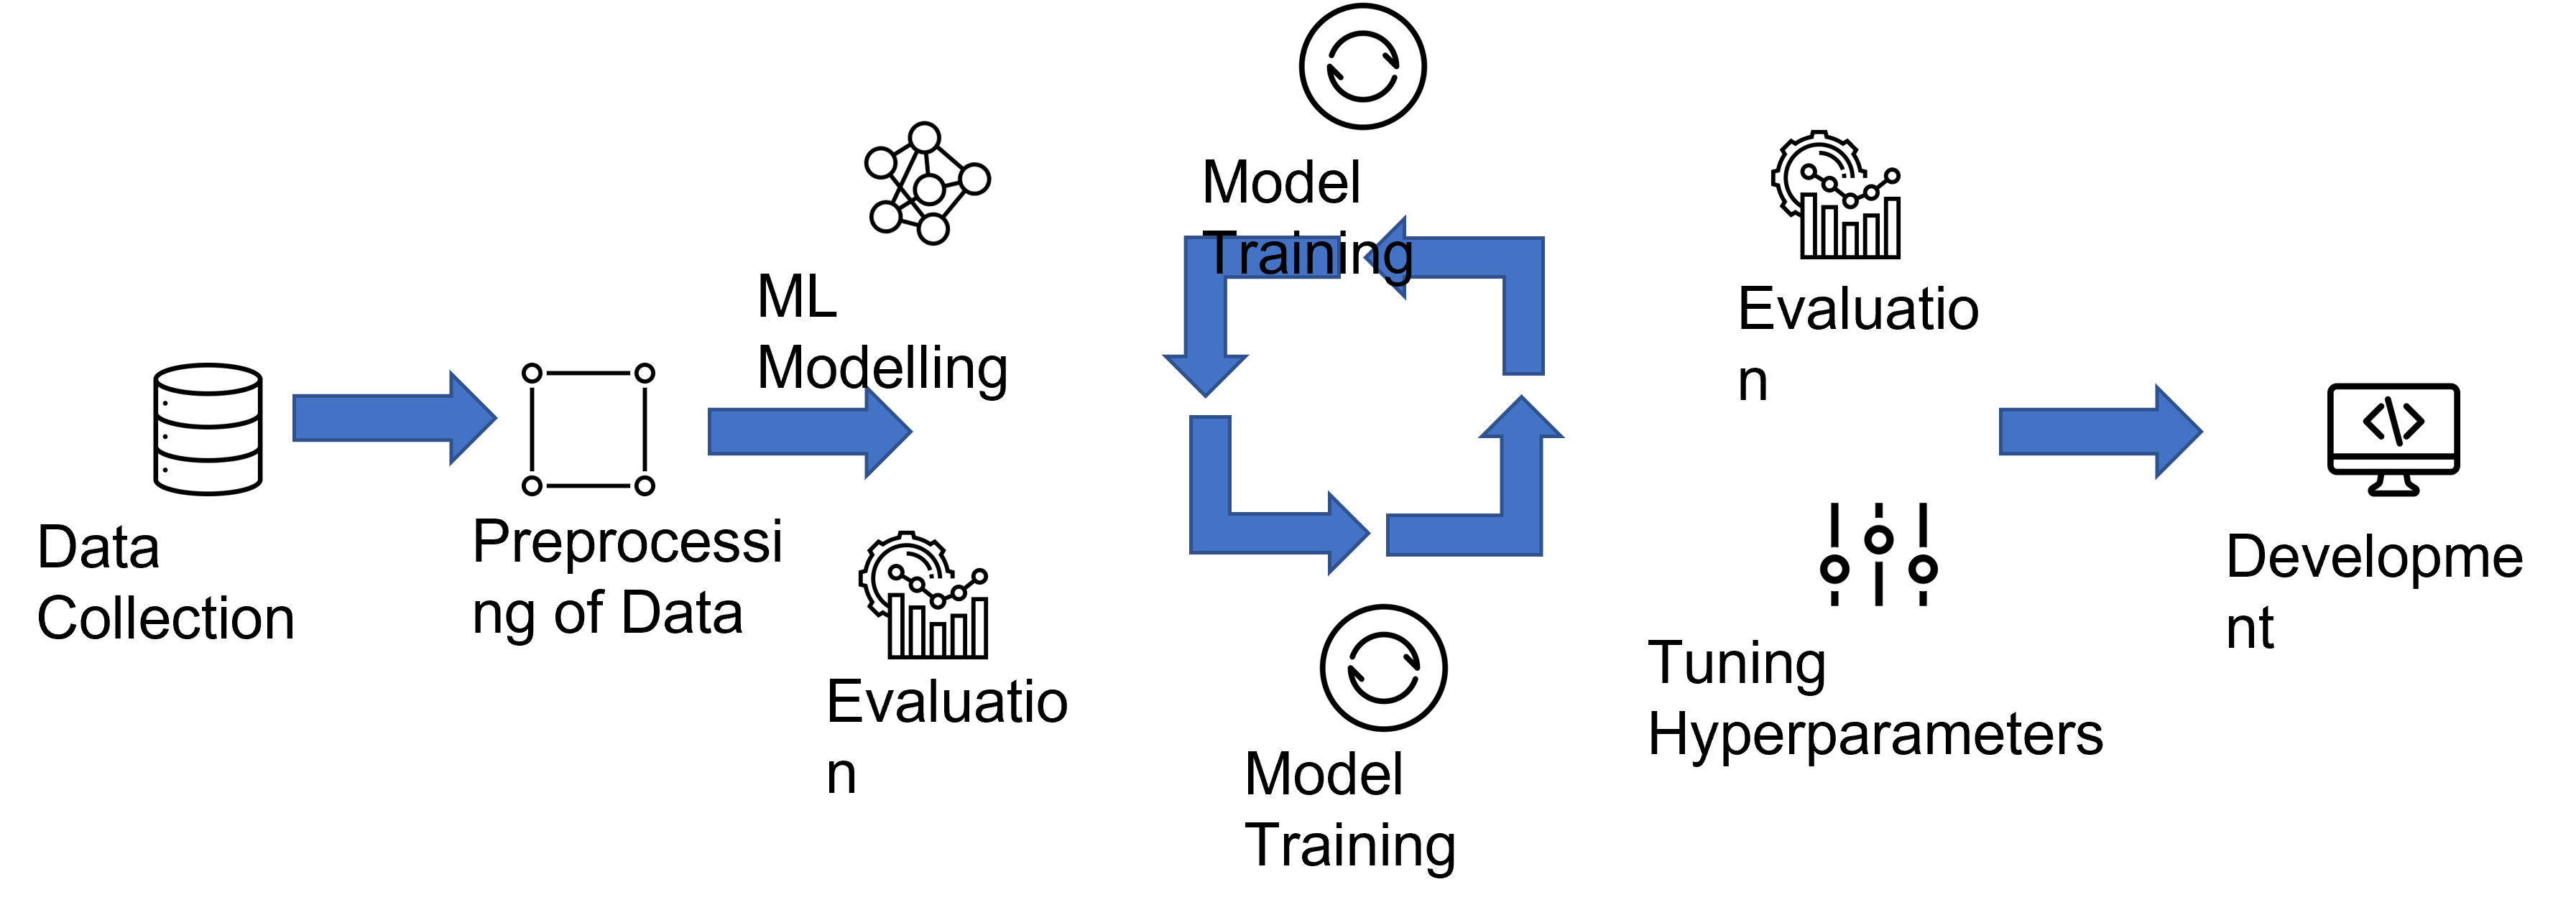
\includegraphics[width=1.0\textwidth]{img/model_centric_ml.png}
    \caption{Model Centric Model Workflow}
    \label{fig:model-centric-workflow}
\end{figure}

\subsection{Why are majority of AI applications model-centric?}
The majority of AI applications are currently model-centric, a possible reason being that AI industry pays close attention to academic research on models. Since it is difficult to create large data-sets which can become widely accepted standards, more than 90\% of AI research papers are model-centric \cite{deeplearningai_data-centric_2021} (\ref{sub:security_privacy_asr_research}). The Code becomes the major focus and data-set is frequently overlooked which is why data collection and pre-processing is considered as a one-time event.

\subsection{Problems with Model Centric Approach}
This approach may be useful for some industries like marketing and advertisement. Google, Facebook, Amazon etc have huge amounts of data with a proper data pipeline and a standard format, with immediate feedback and well-funded Data Science and Machine Learning Departments. However other organizations, like healthcare or engineering or textile industries, have no Data Collection pipeline and MLOps Teams, and hence various issues arise:
\begin{enumerate}
    \item Requirement of highly customized solutions. 
    \begin{itemize}
        \item Unlike Google Ads, a manufacturing company with multiple line of products cannot apply one Model for all products to detect production errors in them.
        \item  Similarly in ASR scenario, model for one language cannot work on all languages. Every language needs different model. Google may be able to have ML department for each product line but not every company can afford the cost of Data Scientists/ Engineers and MLOps Engineers.
    \end{itemize}
    \item Data Points are Limited. 
    \begin{itemize} 
        \item Every industry does not have multiple data sources or data points. Sometimes, the available data-set itself is small e.g. in cases of a small textile fashion brand or a call center solution with limited calls. 
        \item Not all businesses have an effective data collection and standardisation pipeline. If their ML solution is overly model-centric, they will be necessitated to work with small data-sets (i.e. $102$ - $103$ relevant data points), which are known for producing unsatisfactory results for production standards. A wind turbine company, for example, can detect wear on its wind turbines by analysing drone images if it wants to develop a predictive maintenance solution. Aside from thousands of images of 'healthy' wind turbines, the sample size of images showing actual wear and tear on its surface may be around 100, representing 0.0001\% of an ad company's sample size. Hence, a model-centric approach that focuses on optimising the model architecture rather than the problem of a limited number of relevant images would not produce satisfactory results. Similarly in our scenario, CPLC has a lot of unlabelled data but there is no labeling. Plus, the samples of calls of various emotions are also lacking which means that data standardization itself is a project in itself.
    \end{itemize}
    \item Proof of Concept vs Actual Software Deployed in Production. 
    \begin{itemize}
        \item  There are various types of research claiming things that are not actually deployed in a real-world scenario. E.g. in 2019, it was published\cite{ardila_end--end_2019} that certain solutions were developed to accurately detect tumours at an earlier stage than trained radiologists are able to diagnose.  The reason it is not in every hospital yet is due to a substantial gap between the proof of concept and hospital production software. 
        \item If every hospital used the same machines to create its patients' lung scans and saved these images in a central and easily accessible location, the production software would most likely work as intended. In reality, however, this is not the case. Hospitals use various machines purchased from various manufacturers, built in different years, and therefore have varying scan quality.
        \item It is not possible to simply upload all scans to a system that stores them centrally due to data security concerns for hospitals and the healthcare industry. As a result, hospitals typically face a wide gap, with each hospital having to develop its own ML system to meet its own technical and organisational requirements.
        \item Various studies show effectiveness of ASRs with standard corpora using Neural Networks \cite{georgescu_performance_2021}. However, none of them were deployed for our scenario, so we had to create our ASR from scratch.There have been various studies showing the effectiveness of various speech recognition systems with standard corpora (\ref{sub:ASR_from_scratch}). using Neural Networks. 
    \end{itemize}
   
\end{enumerate}

\subsection{Data Centric Approach}
\label{sub:data_centric_approach}

Imagine a 4-year-old child going to school. He is reads in his book that Sun is the white light spherical object in the sky we see at night and moon is the ball of fire we see in the sky during the day. Imagine how his conversation will be. What kind of references he has? If he reads ahead that Neil ArmStrong was the first man to land on moon, the child would be shocked as to how can humans land on a hot ball of fire? This is what happens when we train ML model on a mismatched or poorly labelled data-set. In the long run, it has many more impacts on the accuracy of ML Models. \cite{fan_impact_2021}

Data is critical in AI research, and developing a strategy that prioritises obtaining high-quality data is crucial. Relevant data is not only rare and noisy, but also extremely expensive to obtain. The idea is that AI should be treated in the same way that the finest materials would be when building a house. They should be evaluated at each level rather than just once.

\begin{figure}[h!]
    \centering
    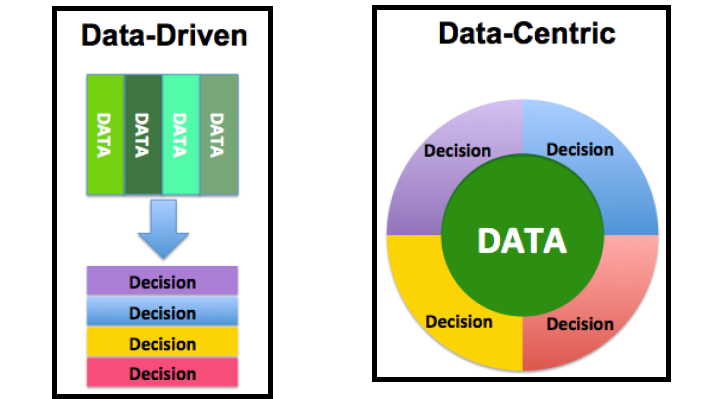
\includegraphics[width=0.8\textwidth]{img/data-centric-ML_2.png}
    \caption{Data Centric vs Data Driven Approaches}
    \label{fig:data-centric-vs-driven}
\end{figure}

\subsection{Data-Centric vs Data-Driven}
There are two approaches with regards to data as shown above -
\begin{itemize}
    \item \textit{Data-centric architecture} is system which treats data as the primary and permanent asset, because applications or ML models change but data is constant. \textit{Data-driven approach} is a method to collect, analyze, and extract insights from data, also known as, “\textit{analytics}.”
    \item \textit{Data-driven architecture} refers to the use of large amounts of data to create technologies, skills, and environments. \textit{Data-centric approach} is centred on using data to determine what should be created in the first place.
\end{itemize}

\begin{figure}[h!]
    \centering
    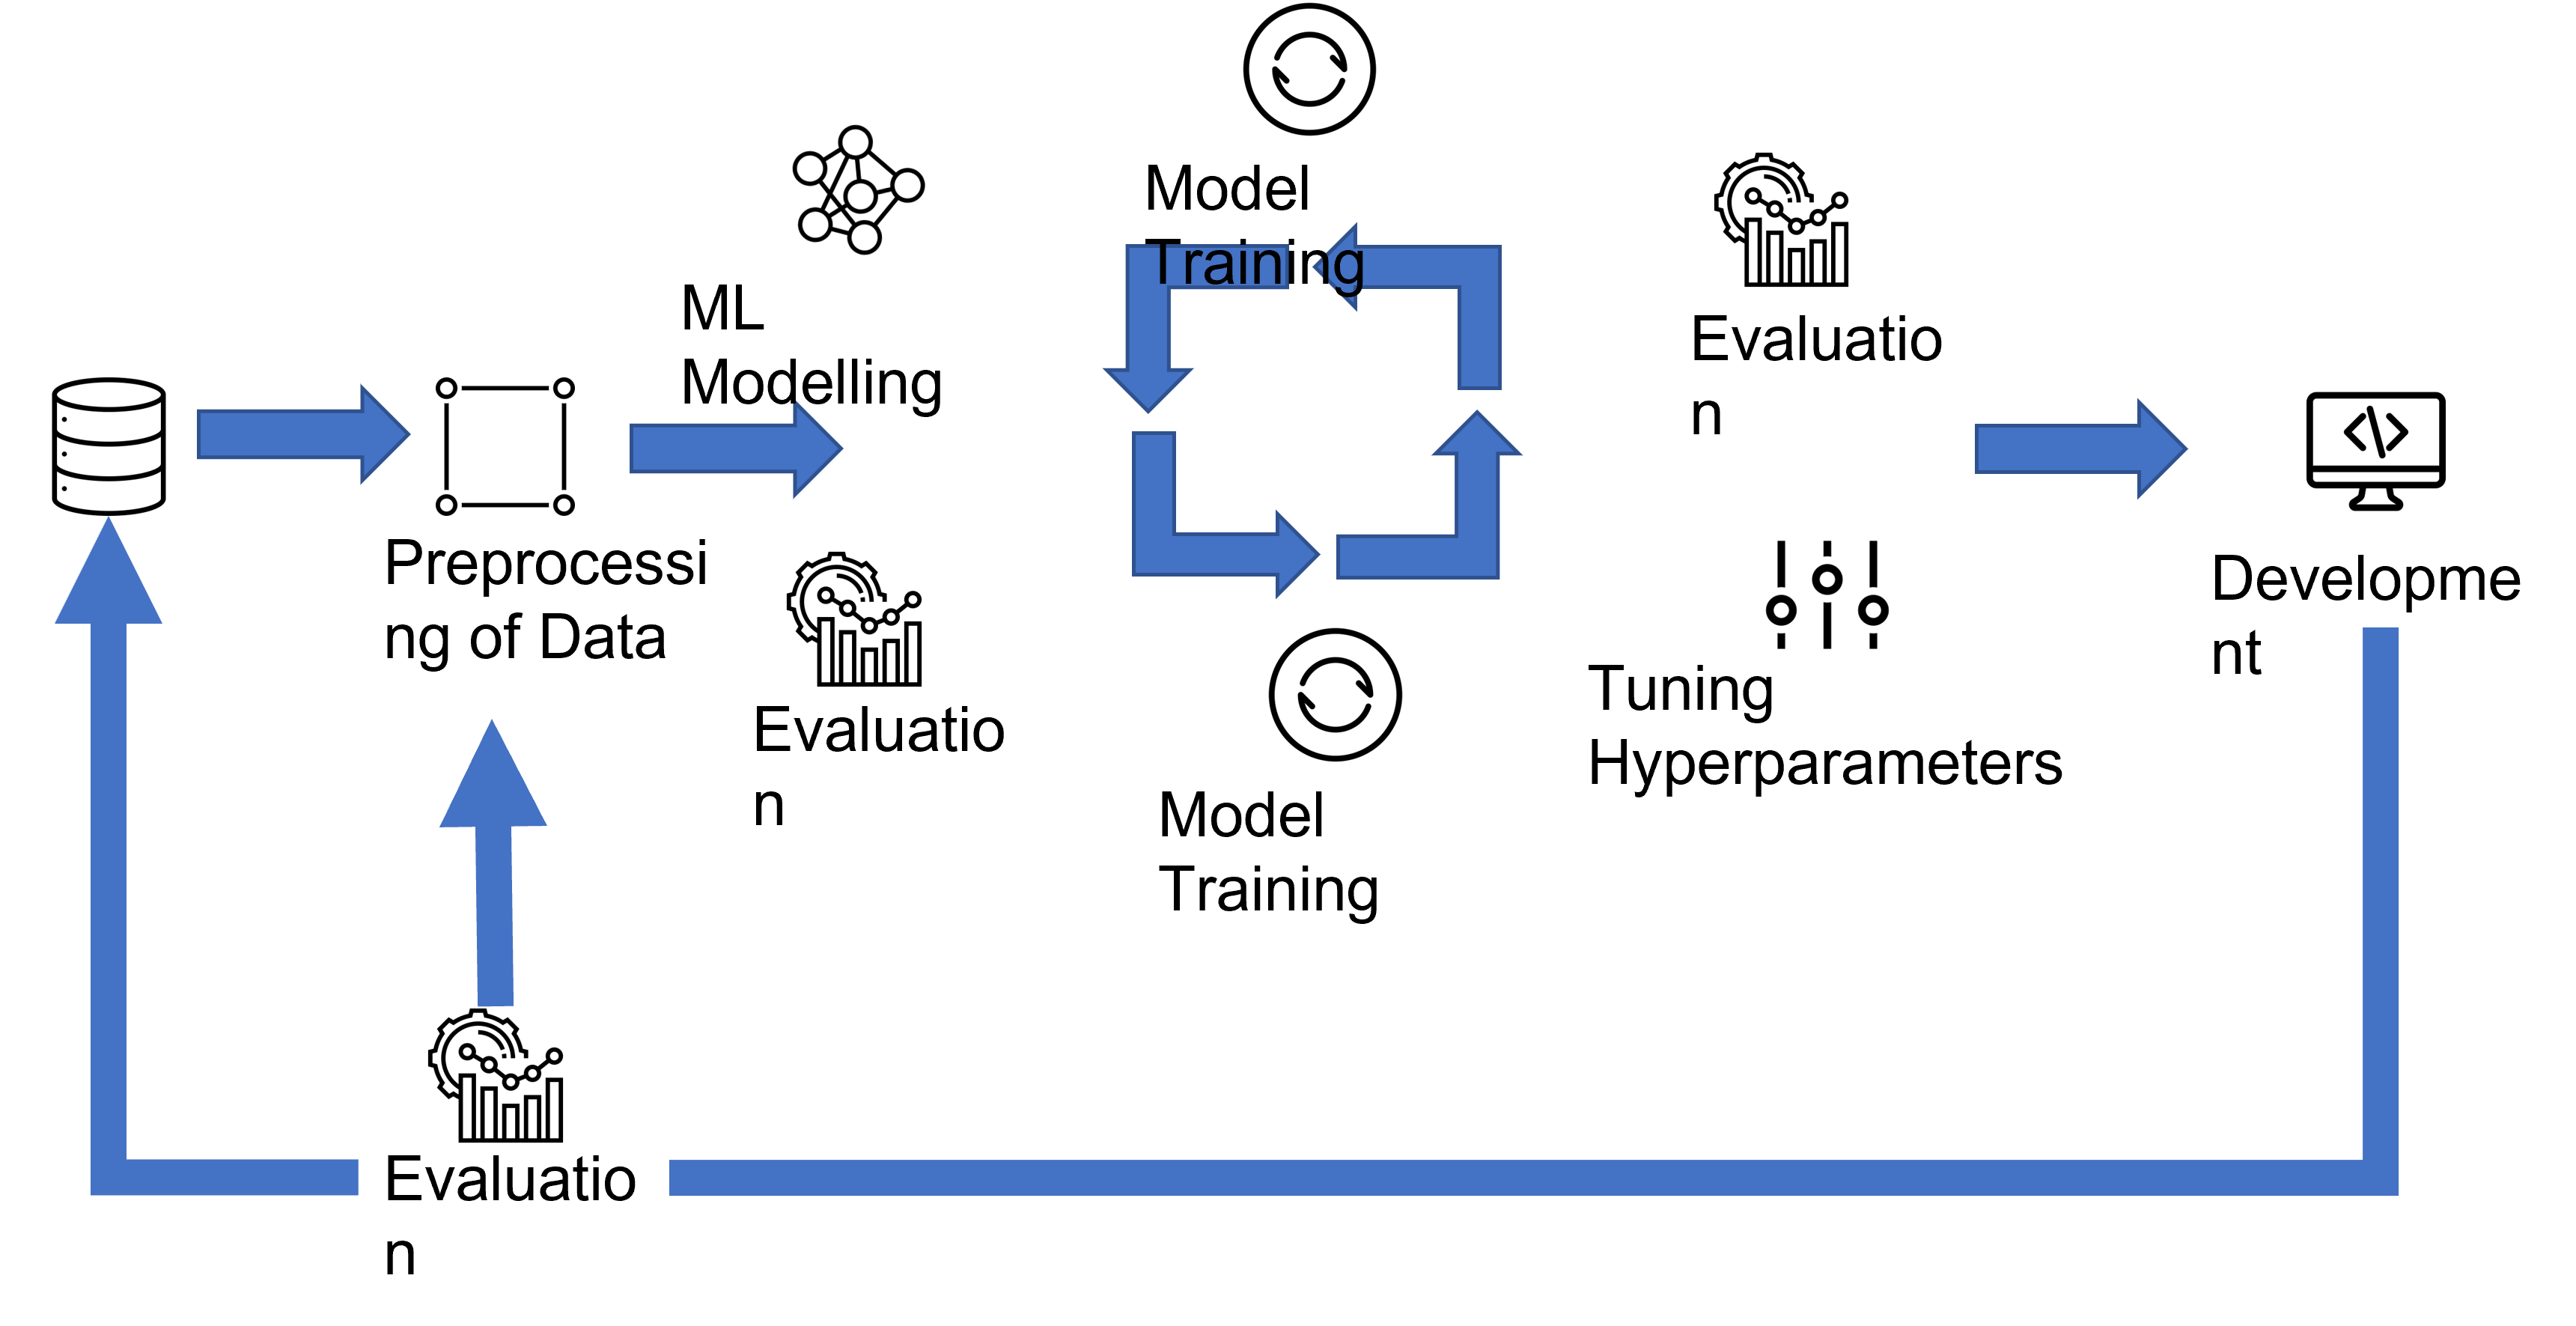
\includegraphics[width=1.0\textwidth]{img/data_centric_ml.png}
    \caption{Data Centric Machine Learning Approach}
    \label{fig:datacentric-ML-approach}
\end{figure}

\subsection{Implementation using Data-Centric Approach}
In the implementation of data-centric approach following steps are important:
\begin{itemize}
    \item Iterative Collection of Data - Data collection is an iterative process in a data-centric approach, particularly for companies that do not have millions of data points or sources, thus, improving the performance of AI systems as well as the quality and quantity of data.
    \item Iterative evaluations for Data Drift Detection - In traditional SDLC, the process may end with the deployment of a specific functionality (ignoring update cycles), but in data-centric ML projects, the ML model will see data that it has never seen before, which will inevitably differ from the algorithm's training data, during production usage. As a result, rather than being a one-time stage, evaluating the model's quality should be an iterative process. Timely feedback from production systems enables recognition and reaction to distributional data drifts and, if required, serves as a prerequisite for online learning. 
    \item Quality Data Labelling: 
    \begin{itemize}
        \item  \textbf{Data labeling} is often done manually which means human errors and biases will exist. If there are inconsistencies w.r.t how the human experts approach particular problem, machines are not likely to detect those inconsistencies.
        \item \textbf{Iterative data collection and high-quality labeling} - These essentially constitute a good data-set for training ML. Huge number of mislabelled audios and transcriptions lead to worse results compared to a small data-set with accurate labeling.
        \item \textbf{Multiple labelers, editors and auditors to spot inconsistencies} - Labelling instructions should be defined and the process to be improved with time and implemented accordingly.
        \item \textbf{Inclusion of domain knowledge and expertise} - This is often missing in scenarios where data labeling is outsourced or not handled with the appropriate amount of precision, care or expertise.
        \item \textbf{Control of labelling annotation process} - Maintaining this helps ensure label quality. The labelling scheme should be well-tested, with clear instructions and labelling quality standards. This gives us more control over the process and allows us to change the labelling scheme as needed. We labelled our data ourselves for this project.
    \end{itemize}
    \item \textbf{Data Augmentation} - It describes techniques for increasing the number of data points in your sample, i.e. the number of defective production parts. It involves: 
    \begin{itemize} 
        \item \textit{Generating the data} that your model has not seen during the training time. Adding data is not the only solution always. E.g. in an image data-set, we can make it rotated, flipped, zoomed, or cropped to create additional different variety in the data-set. In audio data we can play around with the speed of data, make changes to pitch or tone, length, adding silences or extra noises using audio editing tools.
        \item \textit{Removing the noisy observations} or sometimes even adding it, leads to high variance in data which helps the model's ability to generalize better on new unseen data-set.         
    \end{itemize}
    \item \textbf{Data Sources} - Business Logic Must be clear along with source of data when working on MLOps using Data-Centric Approach. Business Logic along with Data Source, data type and other aspects of ML must be integrated to form the best solution. Clarity is required in schemas, data accumulation, business logic to make the data the data storage pipeline consistent and coherrent.
    \item \textbf{Feature Engineering} - It is a machine learning technique which uses available data in a data-set to generate new variables that do not exist in the training set. 
    \begin{itemize}
        \item It can generate new features for supervised and unsupervised learning, aiming to simplify and speed up data transformations while improving model accuracy.
        \item It has a crucial role in introducing the curated features that can bring improvements which otherwise might not exist in raw form since improving  the input data and target$/$ labels improves data quality. For instance, we can change speed, add noise, or overlaps to the audio in training data-set to provide different scenarios for training.
    \end{itemize}     
    \item \textbf{Integration of Domain Knowledge}. 
    \begin{itemize}
        \item ML has to be applied in a certain domain context. E.g. ML applied in hospital scenarios cannot be used in the advertisement. Hence, domain knowledge has a great value
        \item Data engineers and machine learning engineers, labelers, and other non-domain personnel are unable to detect subtle differences, in many cases, that domain experts can.
        \item Domain Experts must be part of the ML Deployment team to make the AI system that gives higher performance and can be deployed in actual scenarios rather than just Proof of Concept.
    \end{itemize}  
\end{itemize}

The common question in this approach is, how much data is enough to build a quality model? We are often told more data a better model. However, in any given scenario, Quality trumps quantity. A data-set with millions of rows with a lot of noisy observations can lead to an obscured learning process, while a smaller data-set with good quality labels tends to give much better results.

\begin{figure}[h!]
    \centering
    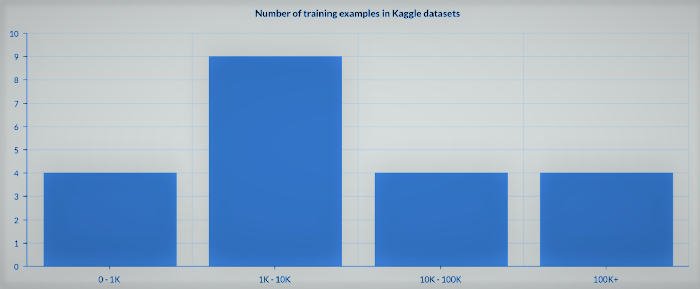
\includegraphics[width=0.9\textwidth]{img/kaggle-dataset.png}
    \caption{Data Quantity (No. of training examples) on Kaggle \cite{patel_data-centric_2021}}
    \label{fig:data-qty-kaggle}
\end{figure}

\begin{figure}[h!]
    \centering
    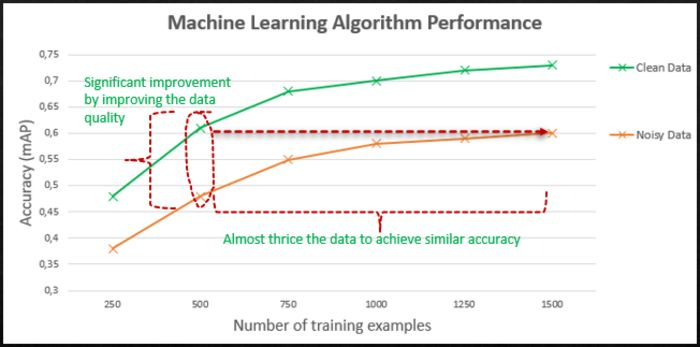
\includegraphics[width=0.9\textwidth]{img/data-centric-ai-3.jpg}
    \caption{ML performance on clean vs noisy (mislabelled) data-set \cite{patel_data-centric_2021}}
    \label{fig:clean-vs-noisy}
\end{figure}

\subsection{Advantages of Data-Centric Approach}
There are numerous advantages to data-centric approach like improved reporting speed and accuracy to better-informed decision-making The benefits of Data-centric infrastructure are as follows:
\begin{itemize}
    \item Improved accuracy by effectively using data as a strategic asset to ensure more precise estimates, observations, and decisions.
    \item Complex data transformations are eliminated.
    \item Data inconsistencies and errors are reduced.
    \item Gives valuable insights into internal and external trends which leads to better decision making.
    \item Expenses are reduced.
    \item Data is made more accessible to key stakeholders.
    \item Data redundancy is reduced.
    \item Data quality and reliability is improved.
\end{itemize}

\section{Methods of ASR Training} 
\label{sec:approaches-asr-trg} 

There are three mainstream Approaches to ASR Model Training: Statistical, End-to-End and Hybrid HMM-DNN Methods. We will now dive deep into each of these approaches, understand their working, weighing their pros and cons which would help select the training method for our ASR.

\begin{figure}[h!]
    \centering
    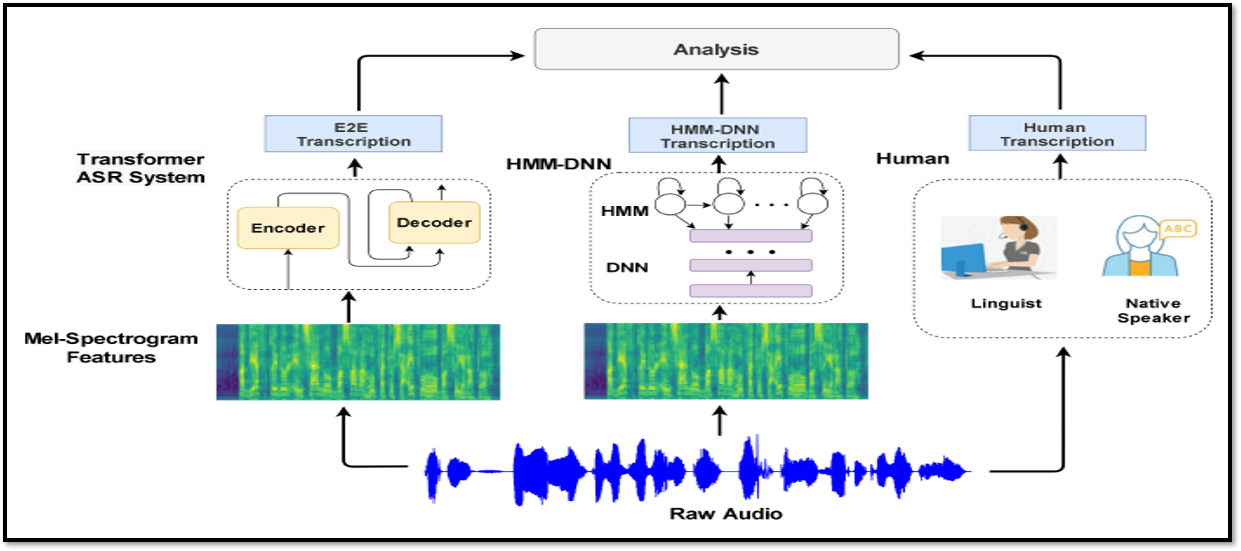
\includegraphics[scale=0.45]{img/ASR-diagram-comparison.png}
    \caption{Traditional, Hybrid vs E2E ASR systems \cite{alsayadi_arabic_2021}}
    \label{fig:Traditional-vs-e2e}
\end{figure}

\newpage

\section{Traditional/ Statistical ASR} 
\label{sec:traditional-asr}

In general, recorded speech is represented as a sequence of acoustic feature vectors or observations, X, and the output sequence of words, W. Our goal at recognition time is to find the most likely W, given X. This is accomplished by training statistical models on a corpus of labelled training utterances ($X_{n}$,$W_{n}$).
\newline
\begin{figure}[ht!]
    \centering
    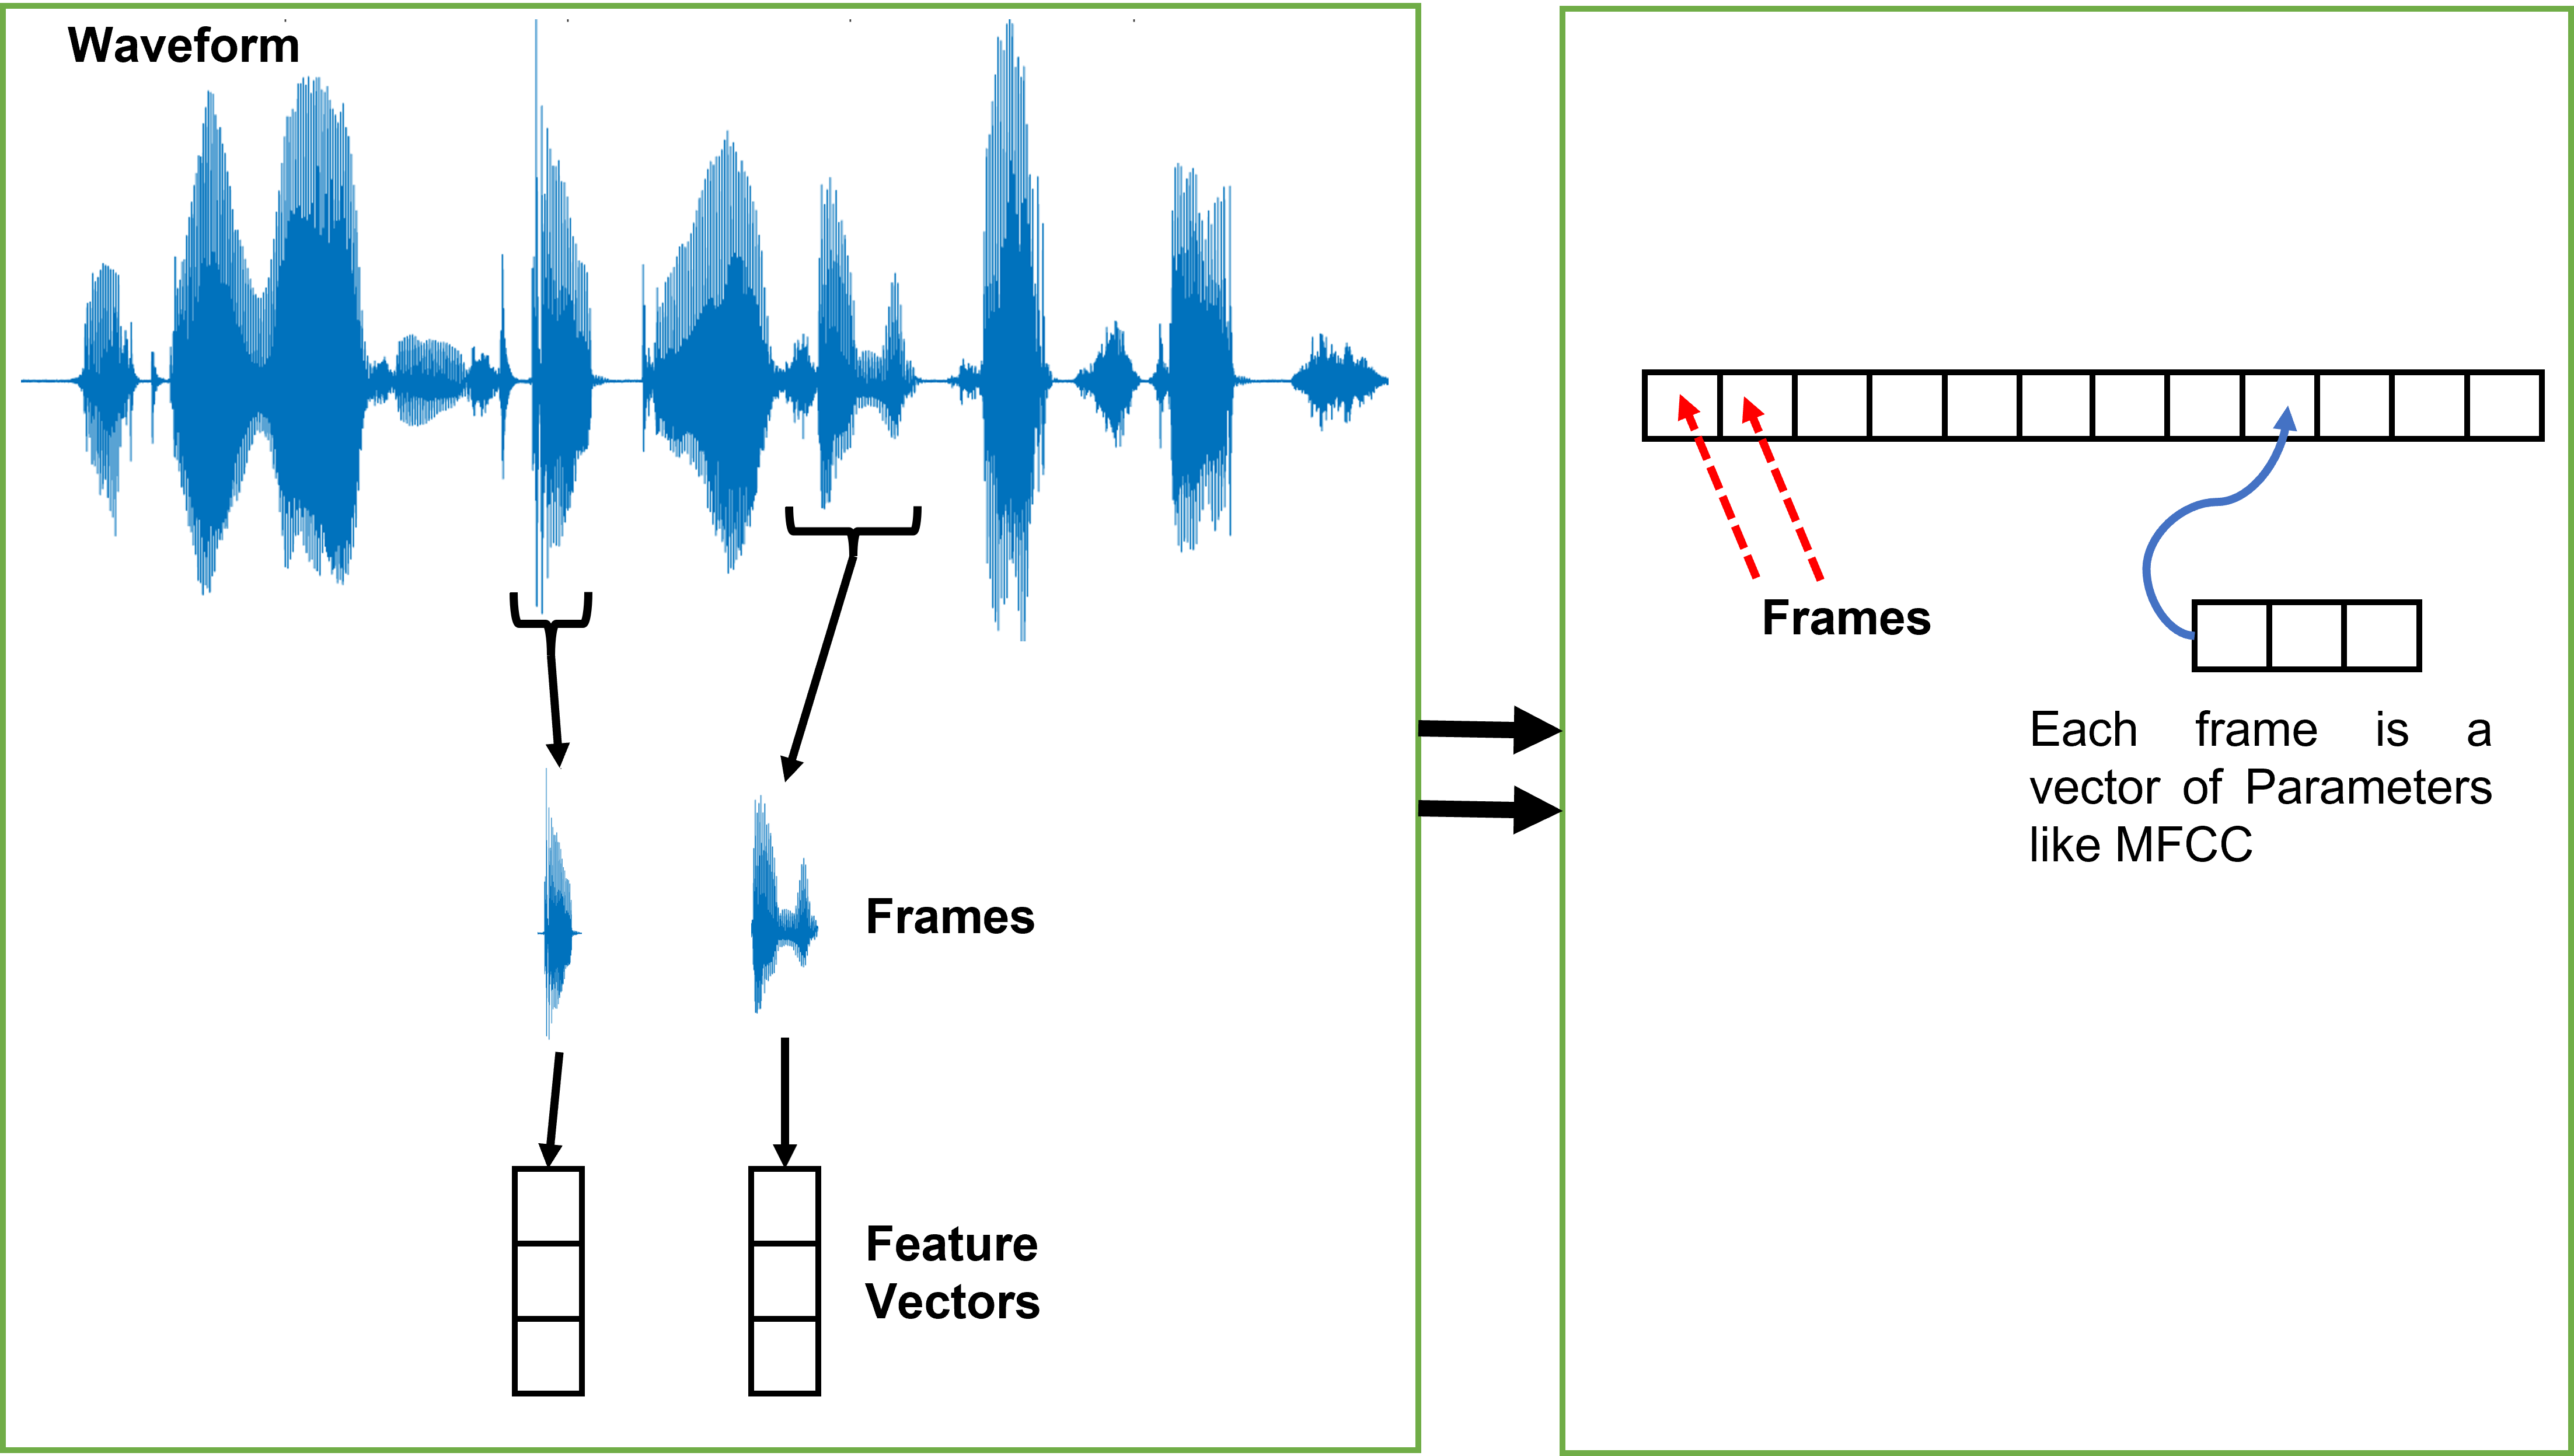
\includegraphics[width=1.0\textwidth]{img/recordedspeechrep.png}
    \caption{Representing Recorded Speech}
    \label{fig:Representing-Recorded-Speech}
\end{figure}
 \newline
Labels (W) may be at different linguistic hierarchical levels like words, phones, etc and they may or may not be time-aligned i.e. alignment as per the start and end times of an acoustic segment corresponding to a label \cite{jurafsky_speech_2009}.
\begin{figure}[ht!]
    \centering
    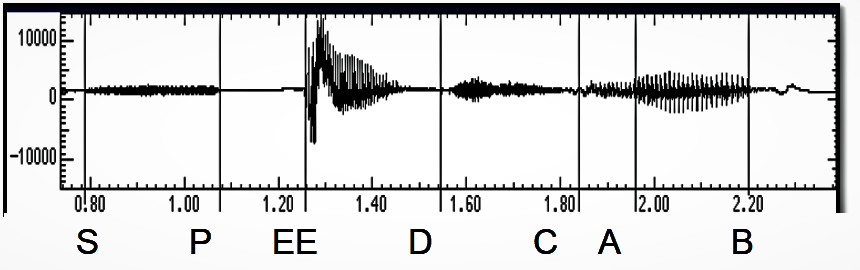
\includegraphics[scale=0.6]{img/speech label.png}
    %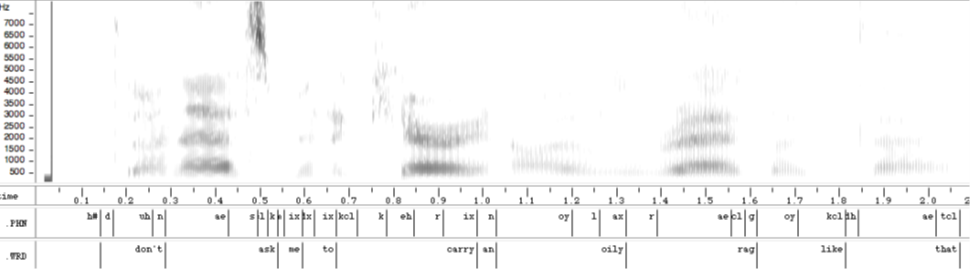
\includegraphics[width=1.0\textwidth]{img/Labelling speech.png}
    \caption{Labelling Recorded Speech}
    \label{fig:labelling-recorded-speech2}
\end{figure}
\newline
The challenge in training the model is aligning the sequences $X_{n}$ and $W_{n}$ for each training utterance, whereas the challenge in recognition is searching all possible output sequences W to find the most likely one.

\begin{figure}[ht!]
    \centering
    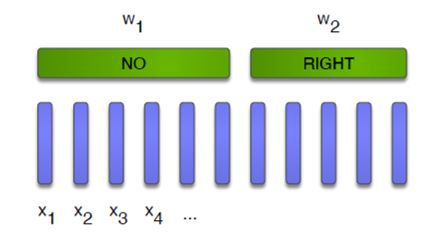
\includegraphics[width=0.7\textwidth]{img/trainingchallenge.png}
    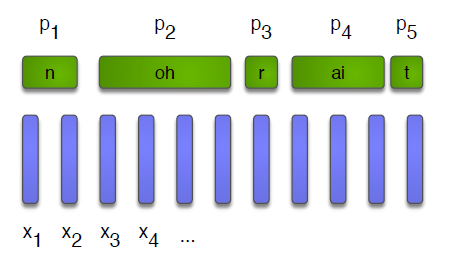
\includegraphics[width=0.7\textwidth]{img/trainingchallenge2.png}
    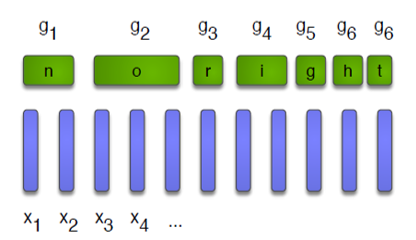
\includegraphics[width=0.7\textwidth]{img/training challenge.png}
    \label{fig:How-Computer-Understands-Words}
    \caption{How computer understands words up to alphabetic or character level using probabilities}
\end{figure}
\newpage
\textit{Hidden Markov Models} assist in mapping continuous observation sequences to discrete output sequences ( generative model for observation sequence). For many years, the HMM-based model was the primary LVCSR model with the highest recognition accuracy. An HMM-based model is divided into three parts: acoustic, pronunciation, and language model. Each model in an HMM-based model is independent of the others and serves a different purpose. While the acoustic model models the mapping between speech input and feature sequence, the pronunciation model maps phonemes (or sub-phonemes) to graphemes, and the language model maps character sequence to fluent final transcription.

\begin{figure}[h!]
    \centering
    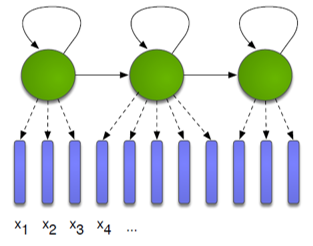
\includegraphics[width=0.6\textwidth]{img/TrASR.png}
    \caption{Finding Word Sequence using HMM}
    \label{fig:word-seq-HMM}
\end{figure}

The most probable word sequence \textit{W*}, given a set of acoustic feature vectors (observations) called \textit{X}, is given by:

\begin{equation}
    W*=\argmax_{W} P(W|X)
\end{equation}

Applying Bayes Theorem: 

\begin{equation*}
    P(W|X)=\frac{P(X|W)P(W)}{P(X)} \\
    \propto P(X|W)P(W) \\
\end{equation*}

\begin{equation}
    W*=\argmax_{W}p(X|W) P(W) \\
\end{equation}
    
where P(X|W) is the acoustic model and P(W) is the language model

Thus, we employ the Acoustic Model, Language Model, and Lexicon to determine the most likely word sequence \textit{W*}, given the observed acoustic \textit{X}.

\begin{figure}[h!]
    \centering
    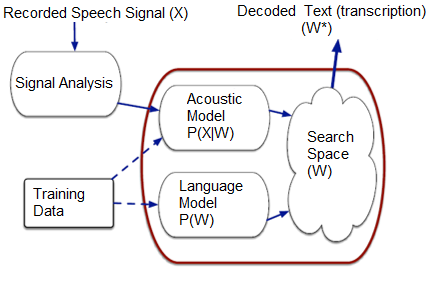
\includegraphics[width=0.6\textwidth]{img/pXW.png}
    \caption{General ASR Architecture}
    \label{fig:basic_asr-arch}
\end{figure}
% https://speechprocessingbook.aalto.fi/Recognition/Speech_Recognition.html


\subsection{Acoustic Model}
\label{sub:acoustic_model}
The observation probability is generally represented by GMM in the acoustic model. The DNN method can compute the posterior probability distribution of the hidden state. These two distinct calculations yield two distinct models, HMM-GMM and HMM-DNN. The HMM-GMM model served as a foundation for many speech recognition systems.

However, as deep learning technology advances, DNN is being used in speech recognition for acoustic modelling. In place of the traditional GMM observation probability, DNN was used to calculate the posterior probability of the HMM state. And hence, the HMM-GMM model is replaced by HMM-DNN because HMM-GMM produces better results than HMM-GMM and thus becomes the state-of-the-art ASR model. Different modules in the HMM-based model use different technologies and play different roles. While HMM is primarily used to perform dynamic time warping at the frame level, GMM and DNN are used to compute the emission probability of HMM hidden states.

\subsection{Pronunciation Model}
\label{sub:Pronounciation_model}

Its primary goal is to establish a link between the acoustic and language sequences. There are various levels of mapping in the dictionary, such as pronunciation to phone and phone to tri-phone. The dictionary is used to map the probability calculation relationship and to achieve structural mapping.

\subsection{Language Model}
\label{sub:language_model}

It contains basic syntactic information with the goal to forecast the likelihood of specific words occurring sequentially in a given language. Language models based on n-grams are commonly used by recognizers. An n-gram contains the prior probability of a word (unigram) or a sequence of words occurring (bigram, trigram etc.):

\begin{itemize}
    \item Unigram probability $P(W_{i})$
    \item Bigram probability $P(W_{i}|w_{i-1})$ 
    \item N-gram probability $P(W_{n}|w_{n-1},w_{n-2},....,w_{1})$
\end{itemize}

\begin{figure}[h!]
    \centering
    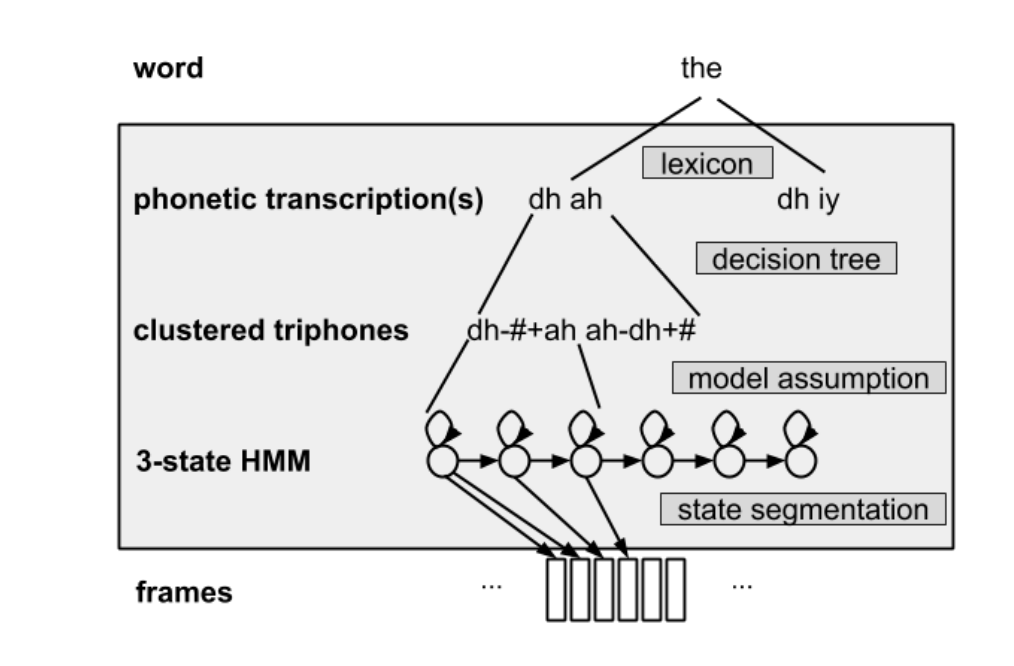
\includegraphics[width=0.6\textwidth]{img/asr_17.png}
    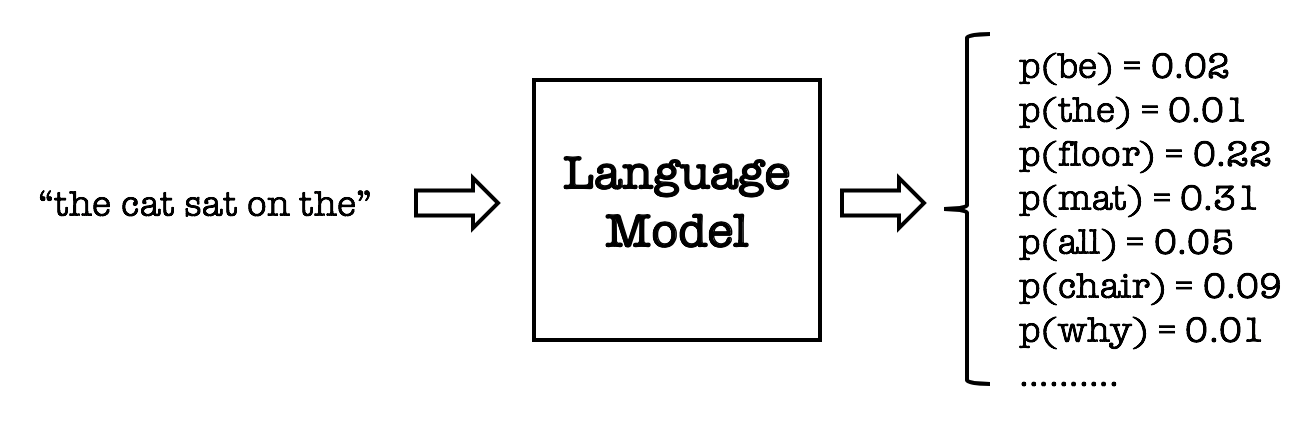
\includegraphics[width=0.6\textwidth]{img/LM2.png}
    \caption{Language Modelling using HMM - tri-phones}
    \label{fig:lang-model2-tri-phones}
\end{figure}

\subsection{Gaussian Mixture Model}
\label{sub:GMM}

Linear regression may be the simplest and most effective data modelling method, especially for estimation of low-dimensional data from high-dimensional data. Beginning with the simplest possible model that provides a good baseline is often a good idea. However, linear models are insufficient in many cases, such as when the data:

\begin{itemize}
    \item is following a non-linear relationship
    \item has inconsistencies or discontinuities 
    \item has multiple classes, each class containing different properties 
\end{itemize}

A relevant class of models includes the Sub-space model, which models the input signal in a lower-dimensional space so that dimensions related to background noise are cancelled while the desired speech signal is retained.

%Moreover, in many cases we are not interested in modelling the average signal, but to recreate a signal which contains all the complexity of the original signal. Say, if we want to synthesize speech, then “average speech” can sound dull. Instead, we would like to reproduce all the colorfulness and expressiveness of a natural speaker. A model of the statistical distribution of the signal can then be more appropriate, such as the Gaussian mixture model (GMM). Similarly if we want to retain the overall speech profile with the noise, this might be the optimum solution.

Whilst approaches like linear regression and sub-space models are based on reduction of dimensionality of a signal to capture the essential information, in many cases we want to model the entire range of possible signals. For that, we can create models of the signal's statistical distribution e.g. a signal can be modelled as a Gaussian process, with each observation having a multivariate Gaussian or normal distribution.

Speech signals, on the other hand, have far more structure than simple Gaussian processes. Voiced signals, for example, differ from unvoiced signals, and within both voiced and unvoiced signals, we have a plethora of distinct groups of utterances with clearly different statistical characteristics. Modeling them all with a Gaussian process would ignore such structures, making the model inefficient.

Mixture models are a type of model in which we assume that the signal under study is divided into several distinct classes, each with its own unique statistical model. For instance, the statistics of voiced sounds differ markedly from those of unvoiced sounds. Each class is modelled by its own distribution, and the joint distribution is the weighted sum of the class distributions. Each distribution's weights correspond to the frequency with which it appears in the signal. So, if unvoiced signals make up 30\% of all speech sounds in some hypothetical language, the weight of the unvoiced class is 0.3.

The most common mixture model structure employs Gaussian (normal) distributions for each of the classes, so the entire model is referred to as a Gaussian mixture model (GMM). They are most common among mixture models because they demonstrate application in an accessible manner. Class-distributions can obviously take other forms than Gaussian depending on the application; for example, if the individual classes follow the Beta distribution, a Beta mixture model could be used. 

We can define a multivariate normal distribution for the variable $x$ as:
\begin{equation}
    f(x;\Sigma,\mu) = \left(\frac{1}{\sqrt{(2\pi)^N ||\Sigma||}}\right) exp\left[-\frac{1}{2}(x-\mu)^T\Sigma^{-1}(x-\mu)\right]
\end{equation}
where $\mu$ and $\Sigma$  are the mean and covariance of this process with N dimensions, respectively. That's the Gaussian process for vectors $x$.

Then we assume we have $K$ classes in the given signal, in which each class has its own covariance $\Sigma_{k}$ and mean $\mu_{k}$. Gaussian Mixture Model for this will be defined as:
\begin{equation}
    f(x)=\sum_{k=1}^{K} \alpha_{k} f(x;\Sigma_{k},\mu_{k})     
\end{equation}

where the weights $\alpha_{k}$ add up to unity $\sum_{k=1}{K} \alpha_{k} = a$

\subsection{Viterbi Algorithm}
The Viterbi algorithm is a dynamic programming algorithm for calculating the maximum a posteriori probability estimate of the most likely sequence of hidden states, also known as Veterbi Path, resulting in a sequence of observed events, particularly in the context of Markov information sources and hidden Markov models (HMM). The acoustic signal is regarded as the observed sequence of events, and a string of text is regarded as the acoustic signal's "hidden cause." Given an acoustic signal, the Viterbi algorithm finds the most likely string of text. \cite{muller_fundamentals_2021}

Some examples of application of this include:
\begin{itemize}
    \item In recognition or classification applications, we can model a system with two distinct states, such as speech and noise, and train a GMM with mixture components that correspond to those states. When we receive a microphone signal, we can calculate the likelihood of each mixture component and thus determine whether the signal is speech or noise.
    \item In transmission applications, our goal is to model the signal so that we can transmit likely signals with few bits and unlikely signals with many bits. We can train a GMM on a speech database to determine which signals are speech-like and can be transmitted with a small number of bits.
\end{itemize}

\subsection{Advantages}
\label{sub:traditional-asr-advantages}

\begin{itemize}
    \item For under-resourced languages speech data where available data is as scarce as 30 hours, statistical models yield a reasonable measure of performance\cite{naeem_subspace_2020}.
    \item Rich and Robust mathematical framework\cite{morgan_continuous_1995}.
    \item Effective methods for learning and decoding.
    \item Provides good abstractions for sequences and temporal aspects.
    \item Topology that is adaptable and flexible for statistical phonology and syntax.
    \item The underlying theoretical basis is much more sound, elegant and easy to understand.
    \item It is easier to implement and analyze.
    \item HMM taggers are very simple to train (just need to compile counts from the training corpus).
    \item Statisticians are comfortable with the theoretical base of HMM.
    \item Performs relatively well (over 90\% performance on named entities).
    \item Liberty to manipulate the training and verification processes.
    \item Mathematical / theoretical analysis of the results and processes.
    \item Incorporates prior knowledge into the architecture with good design.
    \item Initialize the model close to something believed to be correct.
    \item It eliminates label bias problem.
    \item It has also been proved effective for tasks other than ASR like speech recognition, handwriting recognition and sign language recognition.
    \item Because each HMM uses only positive data, they scale well; since new words can be added without affecting learnt HMMs.
\end{itemize}

\subsection{Limitations}
\label{sub:limitations-traditional-asr}
\begin{itemize}
    \item \textit{Complex and Difficult Training process for global optimization} - To train different modules, HMM-based models frequently use different training methods and data sets. Each module is optimised independently, with its own optimization objective functions that differ from the actual LVCSR performance evaluation criteria. As a result, the optimality of each module does not always result in global optimality, and they do not include joint loss optimization.
    \item \textit{Conditional independence assumptions} - The HMM-based model uses conditional independence assumptions within HMM and between different modules to simplify model construction and training. This does not correspond to the actual situation of LVCSR (Large Vocabulary Continuous Speech Recognition).
    \item \textit{Language and Acoustic model optimizing their own local output} - Gives the implication that a lot of tiring hand-engineering may be needed to get a good performance.
    %\item Practical requirements for distributional assumptions like uncorrelated features within an acoustic vector, for phone or subphone states, a first order Markov model is assumed etc.
    \item Usually tends to ignore correlation between the acoustic vectors.
    
\end{itemize}

%In order to define joint probability over observation and label sequence HMM needs to enumerate all possible observation sequences.
%Main difficulty is modeling probability of assigning a tag to word can be very difficult if “words” are complex.
%It is not practical to represent multiple overlapping features and long term dependencies.
%Number of parameters to be evaluated is huge. So it needs a large data set for training.
%It requires huge amount of training in order to obtain better results.
%HMMs only use positive data to train. In other words, HMM training involves maximizing the observed probabilities for examples belonging to a class. But it does not minimize the probability of observation of instances from other classes.
%It adopts the Markovian assumption: that the emission and the transition probabilities depend only on the current state, which does not map well to many real-world domains.

\section{End to End ASR} 
\label{sec:E2E-asr}

Due to shortcomings of the HMM-based model, as well as the promotion of deep learning technology, an increasing number of works started to look into end-to-end LVCSR. The end-to-end model is a system that directly maps input audio sequences to word or grapheme sequences. First we will delve into Concept of Neural Networks before understanding E2E models themselves.

\subsection{Understanding Neural Networks} 
\label{sub:NeuralNetwork}

An Artificial Neural Network (ANN) is a mathematical model that attempts to simulate the structure and functionalities of biological neural networks. Every artificial neural network starts with a basic building block called an artificial neuron which is a simple mathematical model or function. Its design and functionality are based on observations of biological neurons, which are the basic building blocks of biological neural networks (systems) such as the brain, spinal cord, and peripheral ganglia.

Computational modelling with neural networks began in the 1940s and has since experienced several waves of innovation and subsequent decline. Deep neural networks (DNNs) have recently exploded in popularity, which roughly translates to the network having more layers of non-linearities than previous models. 

This is most likely due to an increase in available computational power and the availability of large data sets. It has fueled a flurry of incremental innovation in all directions, and deep neural networks now outperform any competing method in many modelling tasks.

\subsection{Network Structures}

In principle, neural networks are constructed from simple building blocks, the most common of which is $y=f(Ax+b)$. Input vector is $X$, matrix $A$ and vector $b$ are constants, non-linear function is $f$ such as the element-wise sigmoid, and output is $y$. We often refer to it as a \textit{layer} which can then be stacked after each other. A Network with Three Layers looks like this:

$$y_{1}=f(A_{1}x+b_{1}) $$
$$y_{2}=f(A_{2}y_{1}+b_{3})$$
$$y_{out}=f(A_{3}y_{2}+b_{3})$$

\subsection{Deep Neural Networks (DNNs)}
Deep Neural Network (DNN) are an Artificial Neural Networks comprising of multiple layers between their input and output layers. Many experts define deep neural networks as networks that have an input layer, an output layer and at least one hidden layer in between unlike Shallow Neural Network which has only one layer. Each layer performs different types of sorting and ordering in a process known as "feature hierarchy". Dealing with unlabeled or unstructured data is one of the most important applications of these sophisticated neural networks. Deep neural networks are also referred to as "deep learning" networks because they represent a subset of machine learning in which technologies based on artificial intelligence seek to classify and order data in ways that go beyond simple input/output protocols \cite{backstrom_introduction_2022}.

\begin{figure}[h!]
    \centering
    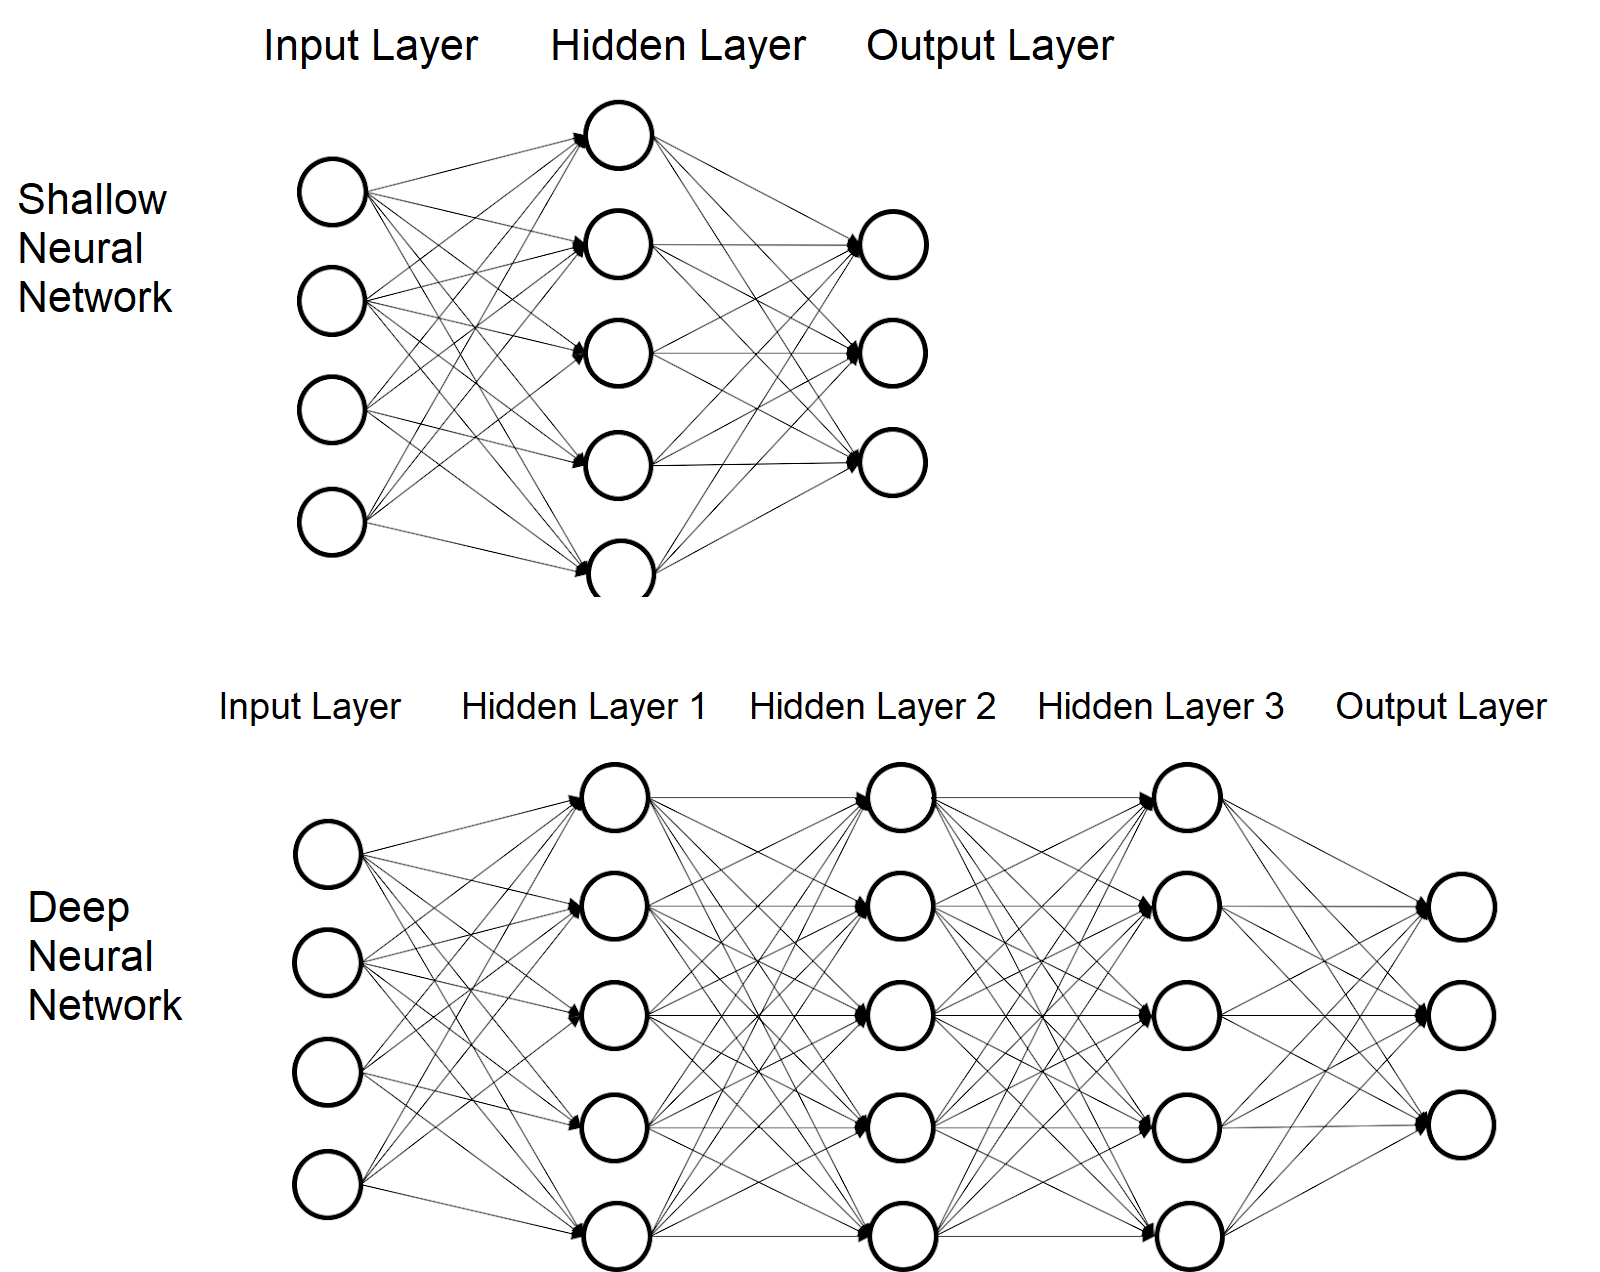
\includegraphics[width=0.7\textwidth]{img/DNN.png}
    \caption{Shallow vs Deep Neural Networks}
    \label{fig:shallow-deep-NN}
\end{figure}

Following are key components of Neural Networks \cite{backstrom_introduction_2022}:
\begin{enumerate}
    \item \textit{Neurons} - It is the fundamental structure of a neural network which simply, receives an input, processes it, and generates an output that is either sent to other neurons for further processing or is the final output.
    \item \textit{Weights} - When a neuron receives an input, it is multiplied by a weight. The weights are initially initialised and are updated during the model training process. After training, the neural network assigns a higher weight value to the input it considers more important than to the input it considers less important.
    \item \textit{Bias} - It is added to the input as the result of weight multiplication and is essentially used to alter the range of the weighted input.
\end{enumerate}

In a neural network, an activation function defines how the weighted sum of the input is transformed into an output from a node or nodes in a neural network layer. Following are types of activation functions in a Neural Network \cite{backstrom_introduction_2022}:
\begin{enumerate}
    \item Sigmoid - It allows for the reduction of extreme or atypical values in valid data without removing them entirely: it converts independent variables with nearly infinite ranges into simple probabilities ranging from 0 to 1. The majority of its output will be close to the extremes of 0 or 1.
    \begin{equation}
        sigmoid(x)=\frac{1}{1+e^{-x}}     \end{equation}
    \begin{figure}[h!]
        \centering
        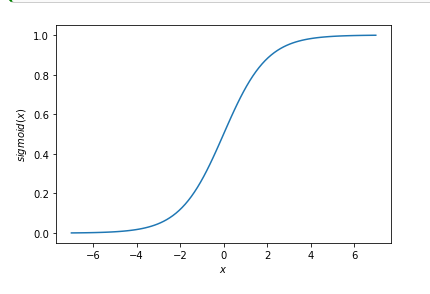
\includegraphics[width=0.5\textwidth]{img/sigmoid.png}
        \caption{Sigmoid Function Graph}
        \label{fig:sigmoid-graphl}
    \end{figure}
    \item ReLU(Rectified Linear Unit) - If the input is less than zero, it produces 0; otherwise, it produces raw output. In other words, if the input is greater than 0, the output is the same as the input. The operation of ReLU is more similar to how our biological neurons work. 
        
        $$ReLU(x)=max(x,0)$$
        $$=x,x>0$$
        $$=0,otherwise$$
     
    \begin{figure}[h!]
        \centering
        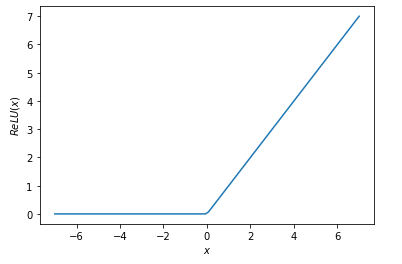
\includegraphics[width=0.5\textwidth]{img/RELU.png}
        \caption{ReLU Graph}
        \label{fig:Relu-graph}
    \end{figure}
    \item Softmax - A variant of the regular max over a vector with a continuous derivative everywhere. In other words, it maps the output to the range [0,1] while simultaneously also ensuring that the total sum is 1. Softmax's output is thus a probability distribution.
    \begin{equation}
      SoftMax(x_{k})=\frac{e^{xk}}{\sum_{j=1}{K}e^{xj}}    
    \end{equation}
    
    \begin{figure}[h!]
        \centering
        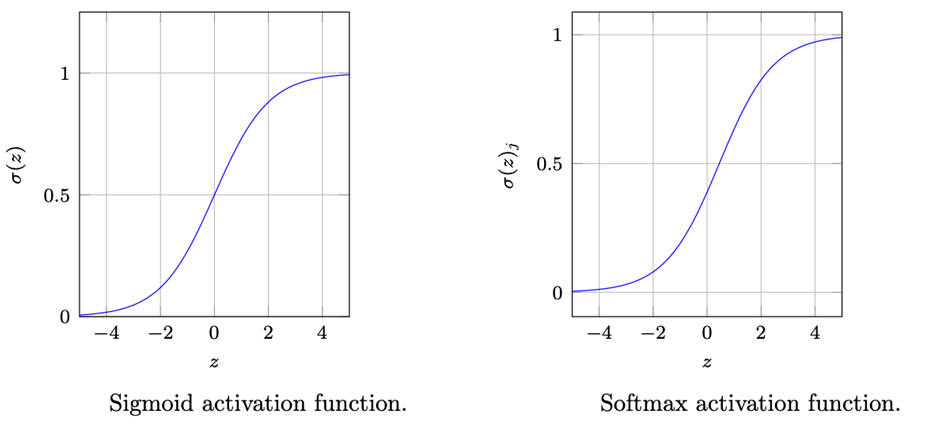
\includegraphics[width=0.9\textwidth]{img/softmax.png}
        \caption{Softmax vs Sigmoid}
        \label{fig:softmax-graph}
    \end{figure}
 
\end{enumerate}

There are some key parameters or components of a Neural Network we need to understand \cite{backstrom_introduction_2022}:
\begin{enumerate}
    \item \textit{Input / Output / Hidden Layer} - The input layer is the first layer of the network and receives input. The output layer is the final layer of the network and is responsible for generating output. The processing layers are the network's hidden layers which are responsible for performing specific tasks on incoming data and passing the results to the next layer. The visible layers are the input and output layers, while the intermediate layers are hidden.
    \item \textit{Multi Layer Perceptron (MLP}- A simplest network consists of input layer, hidden layer and output layer.Each layer contains multiple neurons, and each layer's neurons are all connected to the neurons in the next layer. These networks are also known as completely connected networks.
    \item \textit{Cost or Loss Function} - When we train a network, the main goal is predicting the output as close to the actual value as possible. As a result, the cost/loss function is used to assess this accuracy. When the network makes errors, the cost or loss function penalises it with the aim of running the network to improve prediction accuracy and reduce error, thereby minimizing the cost function.
    \item \textit{Gradient Descent} - An optimization algorithm used to minimise a function by moving iteratively in the direction of the steepest descent as defined by the gradient's inverse.
    \item \textit{Learning Rate} - It is a hyper-parameter controlling the amount of change in the model in response to the estimated error upon update in the model weights and is highly important when confituring a Neural Network. Selection of learning rate is difficult because too small values may result in a long training process which could get stuck, whereas too large value may result in learning a sub-optimal set of weights, along with a training process that is too fast or unstable. Hence, knowing how to investigate the effects of the learning rate on model performance and developing intuition about the dynamics of the learning rate on model behaviour is critical.
    %\item \textit{Back-propagation} - When we define a neural network, we assign random weights and bias values to our nodes. Once we have received the output for a single iteration, we can calculate the error of the network. This error is then fed back to the network along with the gradient of the cost function to update the weights of the network. These weights are then updated so that the errors in the subsequent iterations is reduced. This updating of weights using the gradient of the cost function is known as back-propagation. In back-propagation the movement of the network is backwards, the error along with the gradient flows back from the out layer through the hidden layers and the weights are updated.
    \item \textit{Batches} - During a Neural Network Training we randomly divide the input into several chunks of equal size Instead of sending the entire input in one go. When training data in batches, the model is more generalised than when the entire data set is fed to the network at once.
    \item \textit{Epoch} - It is a single training iteration in both forward and back propagation, of all batches. Thus, one epoch equals one forward and backward pass of the complete input data. It may be highly likely that more number of epochs gives higher accuracy of the network, it takes more time for the network to converge. Moreover, the network might over-fit if the number of epochs are too high.
    \item \textit{Dropout} - This regularization technique used during training in which a number of neurons in the hidden layer are dropped at random in order to prevent the network from over-fitting.
    \item \textit{Batch Normalization} - It adjusts and scales the activations to normalise the input layer e.g. if we have features ranging from 0 to 1 and others ranging from 1 to 1000, we should normalise them to accelerate learning..
\end{enumerate}

\begin{figure}[h!]
    \centering
    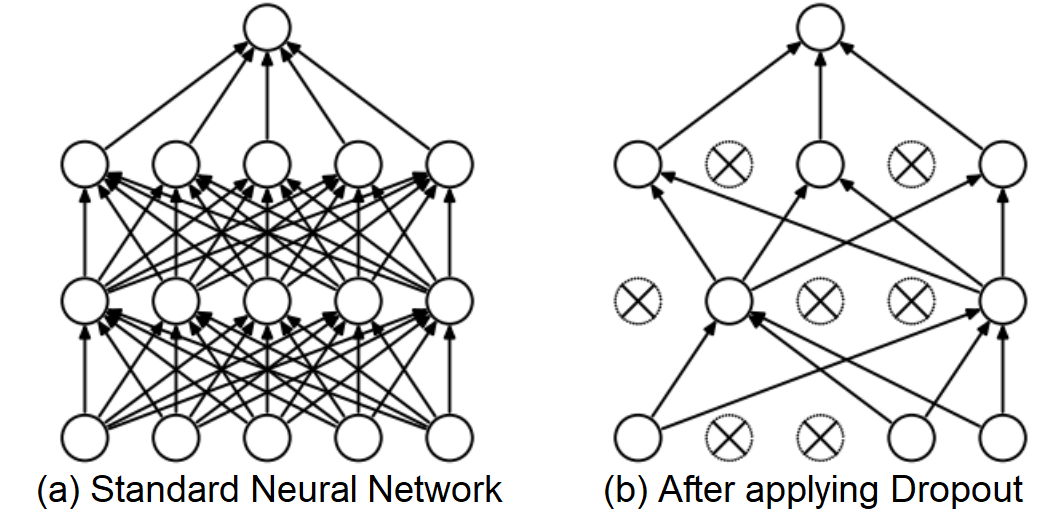
\includegraphics[width=0.9\textwidth]{img/dropout.png}
    \caption{Before and After Dropout}
    \label{fig:droupout}
\end{figure}

\subsection{Forward and Backward Propagation}
Consider a Neural Network containing three inputs X1, X2 and X3, hidden laters with Relu(Rectified Linear unit) activation function which will give zero for any negative value and same value for the positive values the hidden units are H1, H2, H3, H4, H5, and H6 then it has the output layer that will be Y1 and Y2. The neural network also contains biases in our case there are two biases b1 and b2.

\begin{figure}[h!]
    \centering
    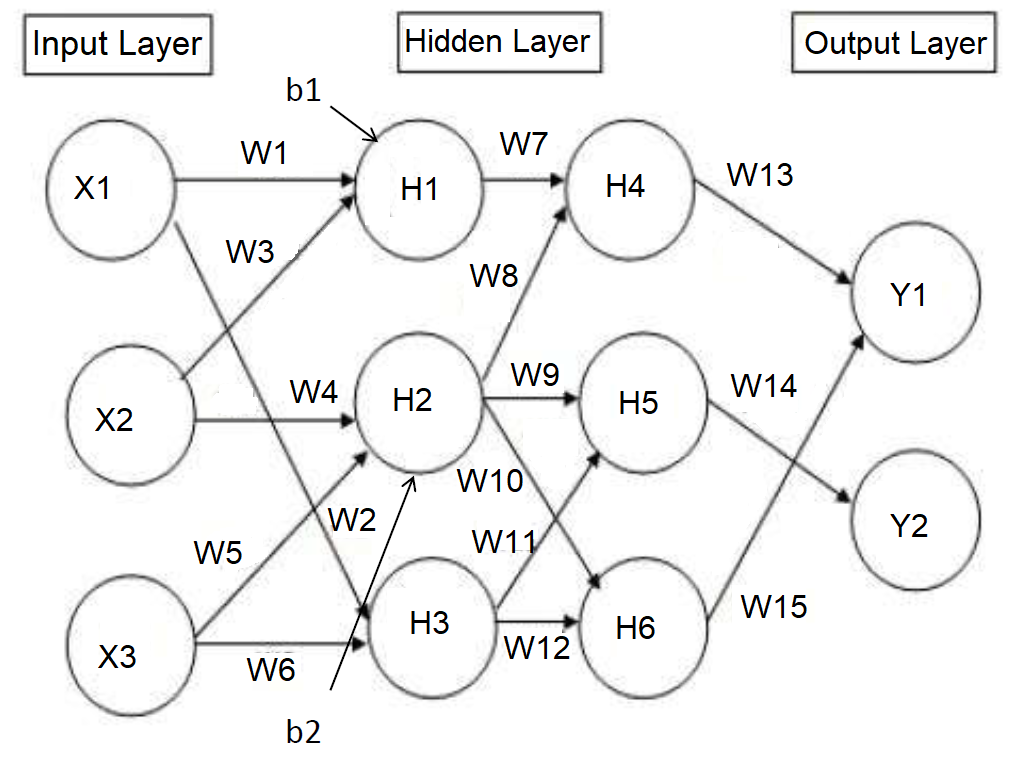
\includegraphics[width=0.7\textwidth]{img/propagation.png}
    \caption{Hidden Layers of NN}
    \label{fig:nn-hiddenlayer}
\end{figure}

\textbf{Forward Propagation}

Forward Propagation is the method used in neural networks to move from the Input layer (left) to the Output layer (right). To achieve the desired values, we will first use forward propagation. We will first compute H1 from the following equation:
\begin{equation}
H_{1}=X_{1}*W_{1}+X_{2}*W_{3}+b_{1}    
\end{equation}

where H1 is an activation function, X1 is the input,W1 is the weight and b1 is the bias. In this way we will calculate H2 and H3. Next we will calculate H4 from the following equation:
\begin{equation}
H_{4}=H_{1}*W_{7}+H_{2}*W_{8}+b_{2}    
\end{equation}

In the same way we will calculate H5, and H6. After calculating all the activation function using input, weights and biases we will then calculate the output Y1 and Y2 using the following equation respectively:

\begin{equation}
 Y_{1}=H_{4}*W_{13}+H_{6}*W_{15}   
\end{equation}
where Y1 is the first output
\begin{equation}
Y_{2} = H_{4}*W_{14}    
\end{equation}

Once the output is calculated we will then calculate the error as we have set our output target. To compute the error we have the following equation:

\begin{equation}
\Xi E_{Total} = \Xi (0.5)(target - output)^2    
\end{equation}

In order to reduce this loss, we will update our weights and for that, we will have to perform backward propagation.

\textbf{Backward Propagation} - Backward Propagation refers to the process of moving from the right to the left, or backward from the Output to the Input layer.

In the Back Propagation weights are updated so as to achieve the target values and to minimize the loss that is calculated by subtracting the output target to the actual target. We will first update the weights of W13 for that we have the following equations
\begin{equation}
\frac{\delta E_{Total}}{\delta W_{13}} = \frac{\delta E_{Total}}{\delta_{out} Y_{1}} \frac{\delta_{out}Y_{1}}{\delta Y_{1}}  \frac{\delta Y_{1}}{\delta W_{13}}     
\end{equation}
 
Now we calculated update $W_{13}$
\begin{equation}
W_{13(Updated)} = W_{13}-\eta \frac{\delta E_{total}}{\delta W_{13}}    
\end{equation}

We will update $W_{14 and 15}$ in this way as well.

Now to second hidden layer to update weights.

\begin{equation}
    \frac{\delta E_{Total}}{\delta W_{7}} = \frac{\delta E_{total}}{\delta_{out} H_{4}} \frac{\delta_{out} H_{4}}{\delta J_{4}} \frac{\delta H_{4}}{W_{7}}
\end{equation}

Now updating the weights
\begin{equation}
    W_{7(Updated)} = W_{7} = \eta * \delta E_{total}/\delta W+{7}
\end{equation}

In this way we will update the weights of $W_{8,9,10,11,12}$. Now we will move to the next layer and will update the weights:

\begin{equation}
\frac{\delta E_{Total}}{\delta W_{1}} = \frac{\delta E_{total}}{\delta_{out}H_{1}}*\frac{\delta_{out}H_{1}}{\delta H_{1}}*\frac{\delta H_{1}}{\delta W_{1}}    
\end{equation}

Updating the weights we get:
\begin{equation}
W_{1(Updated)} = W_{1}-\eta*\frac{\delta E_{total}}{\delta W_{1}}    
\end{equation}

In this way we will update the weights of $W_{2,3,4,5}$. Once all the weights are updated we will then perform forward propagation with the newly updated weights this will reduce our error as we will reach near our targeted value the forward and backward propagation will be repeated again and again until we will achieve our target value.

\subsection{Convolutional neural networks}
\label{sub:CNN}
CNNs were proposed by \cite{fukushima_neocognitron_1988} and used by \cite{lecun_gradient-based_1998}. It is popular used in image classification as well as in Speech technology\cite{abdel-hamid_exploring_2013} \cite{ghahremani_acoustic_2016} \cite{dua_developing_2022}. CNNs have several advantages over DNNs, including the fact that they are highly optimised for processing 2D and 3D images and are effective at learning and extracting abstractions of 2D features. Aside from that, CNNs have far fewer parameters than a fully connected network of similar size.

CNNs are made up of two main components: feature extractors and classifiers. Each layer of the network in the feature extraction module receives the output from the layer immediately preceding it as input and passes it on to the next layer as input. The CNN architecture is made up of three layers: convolution, pooling, and classification.

\begin{figure}[h!]
    \centering
    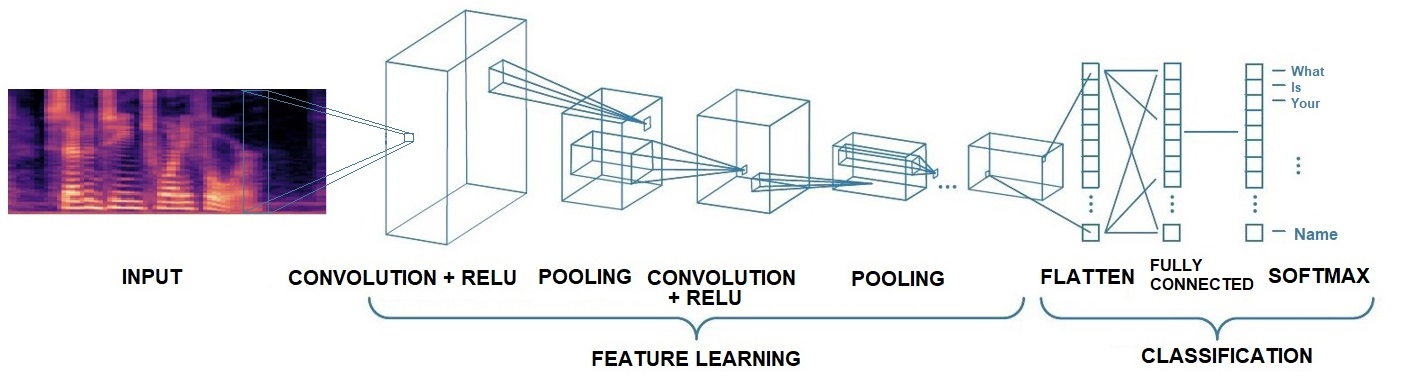
\includegraphics[width=0.8\textwidth]{img/CNN.jpg}
    \caption{CNN Architecture}
    \label{fig:cnn-arch}
\end{figure}

The Layers of CNNs are as follows \cite{abdel-hamid_convolutional_2014}: 
\begin{enumerate}
    \item \textit{Convolutional layer} - A “filter” passes over the image, scans few pixels at a time and creates a feature map predicting the class each feature belongs to. Hence, feature maps from previous layers are convolved with learnable kernels in this layer. To form the output feature maps, the kernels output goes through a linear or non-linear activation function e.g. sigmoid, hyperbolic tangent, Softmax, rectified linear, and identity functions etc. We can combine each output feature map with more than one input feature map.
    \item \textit{Pooling layer} - It reduces the amount of information in each convolutional layer feature while retaining the most important information. (usually there are several rounds of convolution and pooling).
    \item \textit{Fully connected input layer (flatten)} - It takes the previous layers' output and flattens it, turning it into a single vector which can be used as an input for the next stage.
    \item \textit{The first fully connected layer} - Applies weights to predict the correct label, taking inputs from the feature analysis. 
    \item \textit{Fully connected output layer} - It provides final probabilities for each label as output.
\end{enumerate}

High-level features are derived from propagated features from low-level layers. The dimensions of features are reduced As the features propagate to the highest layer or level, respectively on basis of size of the kernel for the convolution and pooling operations. However, the number of feature maps used to represent better features of the input images usually increases to ensure classification accuracy. The final layer of the CNN's output is used as the input to a fully connected network.Feed-forward NNs are utilized as the classification layer because of their better performance \cite{backstrom_introduction_2022}.

\subsection{Components of E2E Models}
End-to-end models of speech recognition typically comprise of the following parts: 
\begin{itemize}
    \item \textit{Encoder} - It maps speech feature sequence from speech input sequence i.e. the aligner realizes the alignment between feature sequence and language.
    \item  \textit{Decoder} - It decodes the final identification result
\end{itemize}

Since an end-to-end system is a complete structure in itself, this division does not always exist. The end-to-end model, unlike the HMM-based model, replaces multiple modules with a deep network, allowing for direct mapping of acoustic signals into label sequences without the use of carefully designed intermediate states. Furthermore, the output does not require performing of posterior processing later \cite{backstrom_introduction_2022}. 

\begin{figure}[h!]
    \centering
    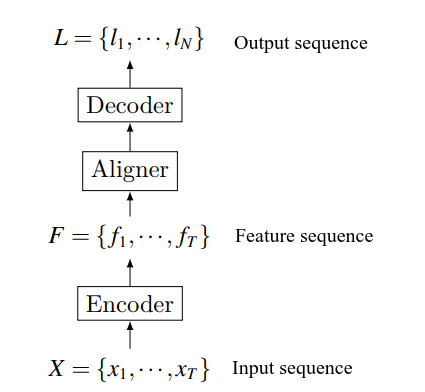
\includegraphics[width=0.6\textwidth]{img/E2E.png}
    \caption{End To End Model Architecture Concept}
    \label{fig:E2E-mathematical}
\end{figure}

\begin{figure}[h!]
    \centering
    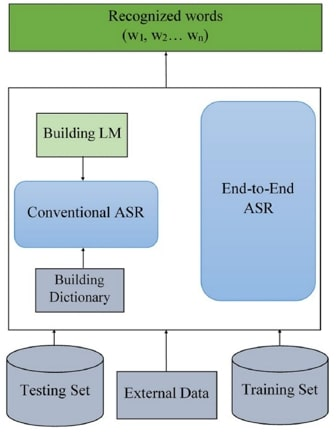
\includegraphics[width=0.6\textwidth]{img/E2EvsConventional.jpg}
    \caption{End To End ASR Workflow vs Conventional ASR Workflow}
    \label{fig:E2E-arch-vs-conventional}
\end{figure}

\subsection{Soft Alignment based Implementations of E2E Models}
\begin{itemize}
    \item \textit{CTC-based} - It starts by listing all of the possible hard alignments. Then, by aggregation of hard alignments, we achieve soft-alignment. When CTC enumerated hard alignments it makes the assumption that output labels are independent of each another.
    \item \textit{RNN-transducer} - It also counts and aggregates all hard alignments as well. When enumerating hard alignments, RNN-transducer, unlike CTC, does not make independent label assumptions. As a result, it is different from CTC in terms of path definition and probability calculation.
    \item \textit{Attention-based} - Instead of enumerating all possible hard alignments, this method employs an attention mechanism to calculate the soft alignment information between input data and output label \cite{backstrom_introduction_2022}.
    
\end{itemize}

\subsection{Advantages}
\label{sub:E2E-advantages}

End-to-end LVCSR has following characteristics\cite{backstrom_introduction_2022}:
\begin{itemize}
    \item For joint training, multiple modules are merged into a single network.The benefit of combining multiple modules is that it eliminates the need for numerous modules to be designed in order to realise the mapping between various intermediate states. Because of the use of joint training, the end-to-end model can use a function that is highly relevant to the final evaluation criteria as a global optimization goal, allowing it to seek globally optimal results.
    \item It directly maps the input acoustic signature sequence to the text result sequence, with no additional processing required to improve recognition performance or achieve true transcription. However, in HMM-based models, for pronunciation of a character chain, there is usually an internal representation. Simplification in the construction and training of speech recognition models is enabled by features of end-to-end LVCSR model.
    \item E2E models are typically much smaller in size than hybrid models, and they have distinct advantages when deployed to device. While we can possibly adapt individual user's model on the cloud and then push it back to individual device, adapting the model on the device is more practical, which requires adjusting the adaptation algorithm to overcome the challenge of limited memory and computation power.
    \item CTC enables the full use of DNN in speech recognition and the development of end-to-end models, which is a significant step forward in the development of end-to-end methods. CTC is a loss function that solves the hard alignment problem while calculating the loss. For end-to-end LVCSR models, CTC primarily addresses the common challenges:
    \begin{itemize}
    \item \textit{Data alignment problem} - CTC does not, any longer, requires training data segmentation and alignment, solving the alignment problem, allowing use of DNN to model time-domain features, greatly expanding DNN's role in LVCSR tasks.
    \item \textit{Directly output the target transcriptions} - Traditional models frequently generate phonemes or other small units, necessitating additional processing to produce the final transcriptions. By eliminating the need for small units and direct output in final target form, CTC greatly simplifies end-to-end model construction and training.
    \end{itemize}
\end{itemize}

\subsection{Limitation}
\label{sub:e2e-limitation}

Despite its triumphs, the application of DNNs in speech processing is not without its drawbacks \cite{backstrom_introduction_2022}:

\begin{itemize}
    \item Training DNNs for a specific task on a particular data set is a black box and does not always improve our understanding of the problem. How will we know if the model is reliable? A trained speech recognizer in language "A" teaches little about speech recognition in language "B" although the designing process of recognizers does teach us about languages.
    \item DNN training is sensitive and specific to the data (and its context) it is trained on. Models can be susceptible to hidden biases such that performance reduces in scenarios of certain under-represented groups of people.
    \item A trained DNN can be a solution to a specific problem, but it does not tell how good the solution it is. For instance, if a data-set represents a 2-D plane circle, then it is possible to accurately model that data-set with NN where the non-linearities are sigmoids. The NN has to be  just large enough to do the job. However, when compared to the equation of the circle, the network is then several orders of magnitude more complex i.e. even though network was successfully trained, and the model is accurate relatively, it provides no indication of whether the network's complexity is comparable to the problem's complexity. 
\end{itemize}

To address such issues, returning to traditional design paradigms has become a recent trend where models are based on a deep understanding of the problem in hand. The parameters of these models are then trained using various  machine learning methods like CTC, RNN etc.

Compared to hybrid approach, E2E modeling is less mature and primarily the research focus on E2E modeling on improvement of general modeling technology. Most of the adaptation technologies successfully applied to hybrid models by adapting acoustic model or language model generally should also work good for E2E models because E2E models usually contain sub-networks corresponding to the acoustic model and language model in hybrid models \cite{bell_adaptation_2020}.

Components in hybrid models are optimised separately, whereas E2E models use a single objective function. Hence, E2E models tend to memorise the training data more, making generalisation or robustness to unseen data difficult for E2E models. Consequently, it is very important to the large-scale application of E2E models to adapt to new environment or new domain.

DNN-based models usually require 1000s of hours of data for training. End-to-end models may need up to 100,000 hours of speech to acheive high accuracy, which is rarely available. For speech, huge amount data (1000 hours or more) is required to good accuracy. It also requires expensive hardware and computational resources. \cite{kincaid_state_2018}

%Uncertainty self-awareness is limited - typical ASR systems always output the most likely word sequence instead of reporting if some part of the input was incomprehensible or highly uncertain
    
CTC has two main deficiencies which hinder its effectiveness \cite{backstrom_introduction_2022}:
\begin{itemize}
    \item Since CTC assumes that output elements are independent of each other, it cannot model inter-dependencies within the output sequence which is why CTC is unable to learn the language model. The CTC-trained speech recognition network should be regarded as merely an acoustic model. In ASR scenario, this has a huge impact. 
    \item CTC can only map shorter input sequences to shorter output sequences making it useless in scenarios where output sequence is longer.
\end{itemize}

To solve the above mentioned issues of CTC, RNN-transducer was proposed. In theory, RNN-Transducer can map an input to any finite, discrete output sequence. Interdependence between input and output elements, as well as within output elements, is also jointly modelled \cite{backstrom_introduction_2022}.

The RNN-transducer has many similarities with CTC \cite{backstrom_introduction_2022}:

\begin{itemize}
    \item Both aim to solve the forced segmentation alignment problem in ASR and introduce a “blank” label. 
    \item They compute the probability of all possible paths and then aggregate them to obtain the label sequence. 
\end{itemize}

Their path generation processes and path probability calculation methods, however, are completely different. This explains why RNN-transducers outperform CTC \cite{backstrom_introduction_2022}.

\section{Hybrid HMM-DNN} 
\label{sec:hybrid HMM-DNN}

Neural networks were first applied to ASR as NN/HMM hybrid systems, which estimated (scaled) likelihoods that act as the HMM state observation probabilities using Neural Network. Both feed-forward networks and recurrent neural networks (RNNs) were used in such hybrid systems in 90s and almost state-of-the-art results were achieved \cite{morgan_continuous_1995}. 

Although context-dependent NN-based acoustic models were also available, these systems were largely context-independent. The computational power of neural network systems at the time was limited, and they were unable to achieve the precise levels of modelling obtained by context-dependent GMM-based HMM systems, which became the dominant approach.

Increases in computational power, on the other hand, enabled deeper neural network models to be learned alongside context-dependent modelling while using the same number of context-dependent HMM tied states (Senones) as GMM-based systems resulting in the development of systems outperforming GMM-based systems in terms of accuracy. The increase in computational power also allowed for the use of more powerful neural network models, such as time-delay neural networks (TDNNs), convolutional neural networks (CNNs), LSTM, RNNs, and bidirectional LSTM \cite{bell_adaptation_2021}.

The figure below shows NN architectures used for hybrid NN/HMM and end-to-end (CTC, RNN-T, AED) speech recognition systems:
\begin{enumerate}[label=(\alph*)]
    \item Scheme of NN in NN/HMM hybrid systems and CTC
    \item RNN Transducer (RNN-T) architecture
    \item Attention based encoder-decoder (AED) end-to-end systems architecture in which $x_{t}$ denotes input acoustic feature vectors; $h_{t}$ and $h_{u}$ denotes hidden layers, and $y_{t}$, $y_{u}$ denotes output labels, depends if they are indexed by time \textit{t} in hybrid and CTC systems or only by output label \textit{u} in parts of RNN-T and AED systems. The encoders use a wide temporal context as input, in practice, even the whole acoustic sequence in the case of most CTC and AED models.
\end{enumerate}

\begin{figure}[h!]
    \centering
    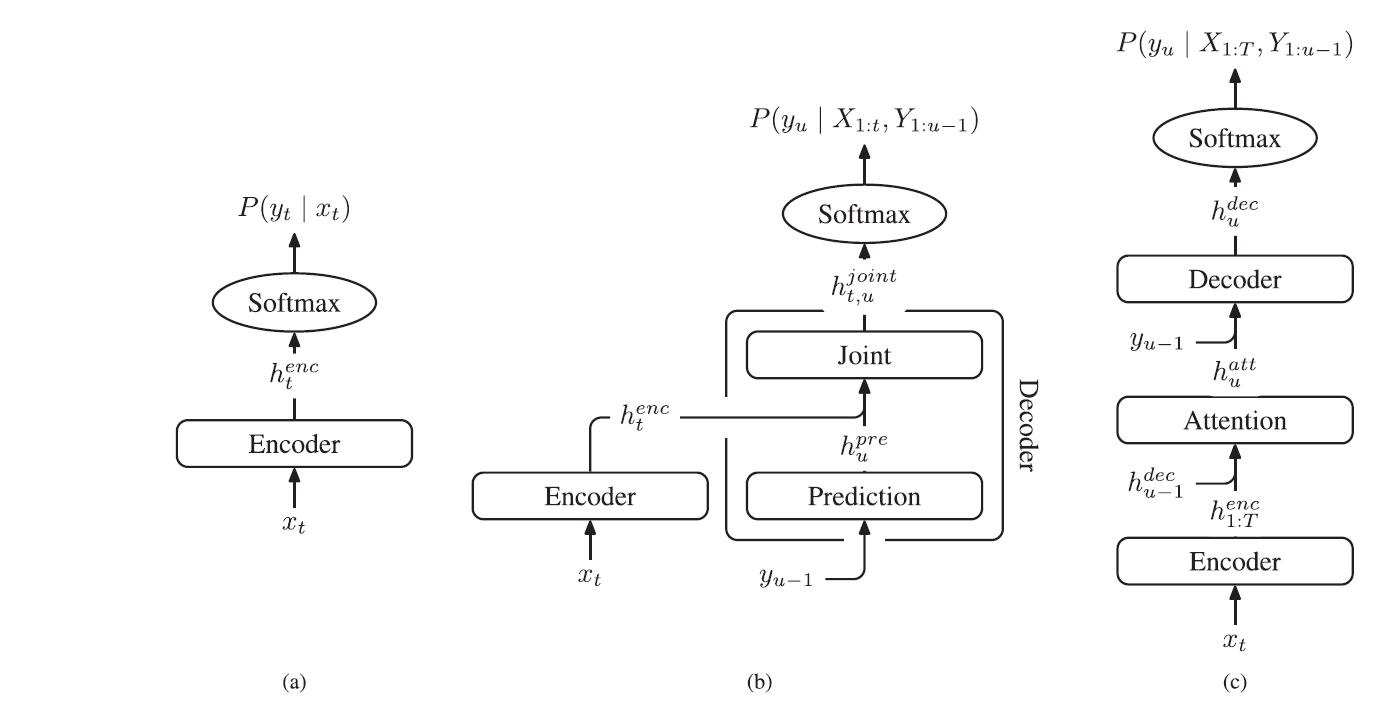
\includegraphics[width=1.0\textwidth]{img/hybridande2e.png}
    \caption{NN architectures for Hybrid NN/HMM and E2E}
    \label{fig:hybrid-e2e}
\end{figure}

\subsection{How does HMM-DNN Hybrid Model work}

Each hidden unit affects the error function indirectly via all the output units which is why hidden units make training weights more complicated. Another problem is the credit assignment problem i.e. what is the hidden unit's "error" and the importance of input-hidden weight $v_{kd}$ to output unit \textit{j}? To solve this, we back-propagate the gradients through the network - the gradient for a hidden unit output with respect to the error can be computed as the weighted sum of the deltas of the connected output units (Propagate the $g$ values backwards through the network). In order to perform gradient descent training, the back-propagation of error (backprop) algorithm enables the propagation of error gradients through a deep network.

\begin{figure}[h!]
    \centering
    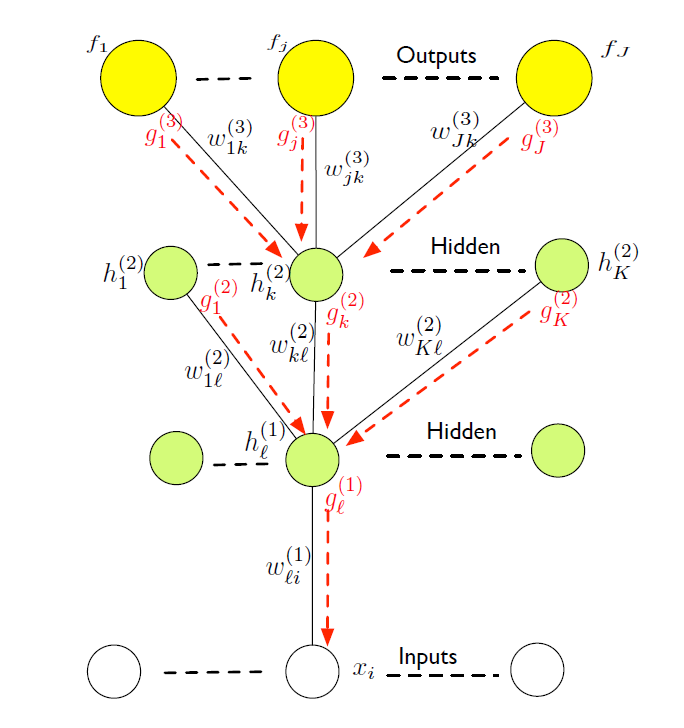
\includegraphics[width=0.7\textwidth]{img/DNN backdrop.png}
    \caption{Training DNN Using Backward Propagation (red-line shows the backward path)}
    \label{fig:dnn-backdrop}
\end{figure}

Take TIMIT Corpus for instance in which \cite{garofolo_john_s_timit_1993}:
\begin{itemize}
    \item 630 speakers each read 10 sentences (usually use 8 sentences per speaker, since 2 sentences are the same for all speakers).
    \item 462 speakers allocated in train-set and 168 for test-set.
    \item Time Aligned speech i.e. speech hand-labelled at the phone level. 
    \item The 61-phone set is frequently lowered to 48/39 phones..
\end{itemize}

The tasks for Phone Recognition would involve: 
\begin{itemize}
    \item \textit{Frame Classification} - Each Data frame is classified.
    \item \textit{Phone Classification} - Each data segment is classified (segmentation into unlabelled phones is given).
    \item \textit{Phone Recognition} - Data is segmented and each segment is labelled which is the usual speech recognition task.
\end{itemize}

Frame classification with a neural network can be accomplished simply by training with labelled frames and testing one frame at a time, assigning the label to the output with the highest score. A neural network is trained to associate a phone-state label with an acoustic data frame and its context. The network's output can be interpreted as P(phone-state | acoustic-frame).

In an HMM-DNN system, we replace the GMMs used to estimate the output probability density function with neural network outputs. Since the HMM system has one state for each phone, we train a neural network as a phone-state classifier (phone-state probability estimator) and use it to obtain output probabilities in the Viterbi algorithm to find the most likely sequence of phones (words).

\subsection{Prosterior Probability Estimation and Neural Networks} 
Suppose we have a Neural Network that has been trained as a classifier, with each output representing a different class. When applied to test data, it can be demonstrated that the value of output corresponding to class j given an input  $x_{t}$, is an estimate of the posterior probability $P(q_{t} = j |x_{t} )$. This is due to the fact that we have soft-max outputs and employ a cross-entropy loss function. We can relate the posterior $P(q_{t} = j | x_{t})$ to the likelihood $p(x_{t} |q_{t} = j)$ used as an output probability in an HMM using Bayes Rule :

\begin{equation}
        P(q_{t}|x_{t})=\frac{p(x_{t}|q_{t}=j)P(q_{t}=j)}{p(x_{t})}    
\end{equation}

\subsection{Scaled Likelihood}
We need the probabilities (or densities) of the form p(x|q) likelihoods in order to use NN outputs as output probabilities in an HMM. Scaled likelihoods can be written as:
\begin{equation}
    \frac{P(q_{t}=j|x_{t})}{p(q_{t}=j)}=\frac{P(x_{t}|q_{t}=j)}{p(x_{t})}
\end{equation}

Scaled likelihoods are obtained by "dividing by the priors" i.e. divide $P(q_{t} = j | x_{t})$ i.e. each network output by the relative frequency of class i.e. $P(q_{t} )$ \textit{j} in the training data. It is better to use $p(x_{t}|q_{t} = j)=p(x_{t})$ instead of $p(x_{t} |q_{t} = j)$ because $p(x_{t})$ is not dependent on the class \textit{j}. Instead of usual likelihoods obtained from a GMM, scaled likelihoods obtained from a neural network are used.

\subsection{The Hybrid System}
\label{sub:hybrid-system}
In general, we train a J-output NN to estimate the scaled likelihoods used in a hybrid system if we have a J-state HMM system. For continuous speech recognition we can use\cite{morgan_continuous_1995}: 
\begin{itemize}
    \item 01 x state per phone - 61 NN outputs, if we have 61 phone classes.
    \item 03 x state context-independent (CI) models - 61 x 3 = 183 NN outputs.
    \item State-clustered context-dependent (CD) models, with one NN output per tied state. Note that this can lead to networks with many outputs.
\end{itemize}

Next, we get Scaled likelihood and "divide by the priors." The scaled likelihoods are computed by factoring out the prior estimates for each phone based on the acoustic training data. Based on the language model and lexicon, the HMM can then incorporate better prior estimates.

\begin{figure}[h!]
    \centering
    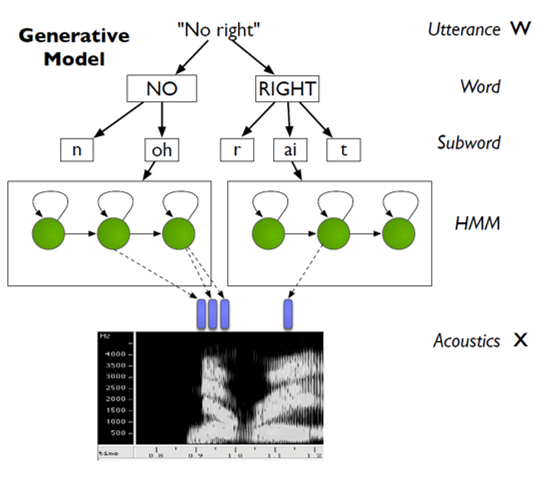
\includegraphics[width=0.6\textwidth]{img/TrASR1.png}
    \caption{Generating HMM}
    \label{fig:Generating-HMM}
\end{figure}

\subsection{DNN Acoustic Modelling}
Let us look into how DNN Acoustic Modelling is done using TIMIT \cite{garofolo_john_s_timit_1993} corpus. To provide training targets (time state alignment) to our DNN, we first train a baseline 3-state mono-phone HMM/GMM system comprised of 61 phones, three-state HMMs, and Viterbi alignment.

DNN has 183(61x3) outputs, and the HMM/DNN system employs the same set of states as the HMM/GMM system. DNN has multiple hidden layers, having more width, employing HMM state alignment as outputs instead of hand-labeled phones - 3-state HMMs (3 x 61phones = 183 states). Take a look at the figure below: 

\begin{figure}[h!]
    \centering
    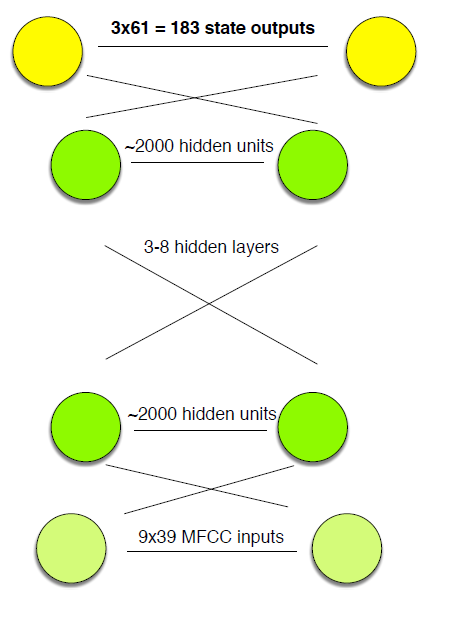
\includegraphics[width=0.5\textwidth]{img/timtdnn.png}
    \caption{DNN layers}
    \label{fig:DNN-layers}
\end{figure}

There is no exact size for a hidden layer, but we usually use 3-8 hidden layers with 1024-3072 units per hidden layer. Training hidden layers necessitates more computational power, requiring the use of a GPU. Multiple hidden layers are always outperform single hidden layer. The best systems have lower phone error rates than the best HMM/GMM systems when using cutting-edge techniques such as SAT and discriminative training.

Filter bank features (spectral domain) are not used because they are highly correlated. They would require either full covariance matrix Gaussians or a large number of diagonal covariance Gaussians. MFCC tends to work better as explained in \ref{sub:MFCC}

\begin{figure}[h!]
    \centering
    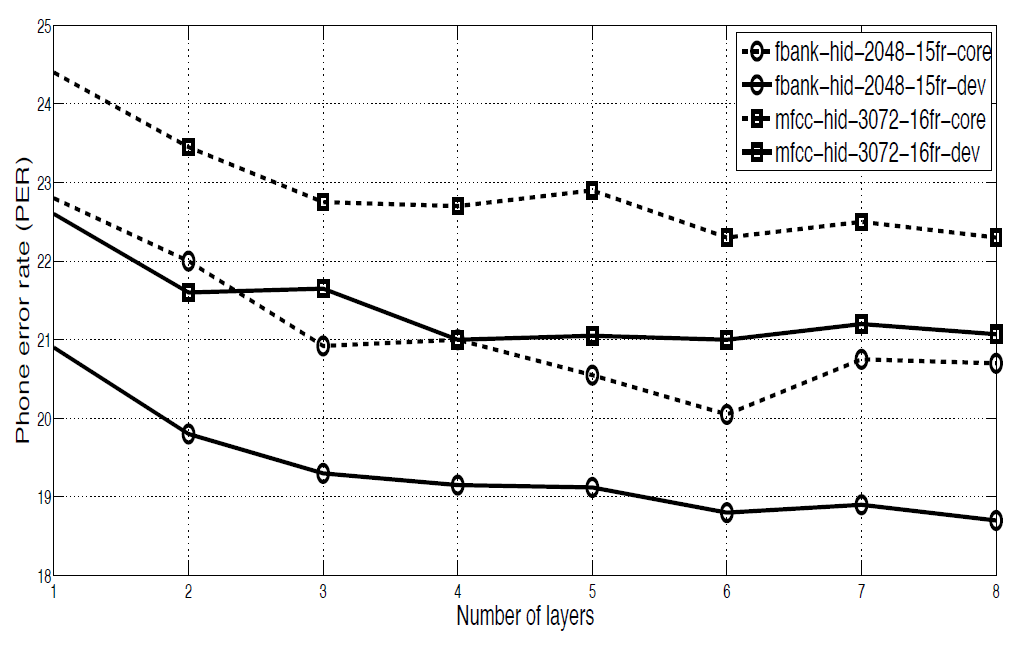
\includegraphics[scale=0.4]{img/fbank vs mfcc.png}
    \caption{Fbank vs MFCC \cite{mohamed_understanding_2012}}
    \label{fig:mfcc-vs-fbank}
\end{figure}

DNNs do not require uncorrelated feature vector components as it can use multiple frames of input context directly. This has been done in NN/HMM systems since 1990 and is critical for them to work well.

\subsection{Tandem Scheme}
The basic idea is to use the Neural Net's output probabilities as input features to the standard CD-HMM-GMM system. It combines the qualities from two approaches: 
\begin{enumerate}
    \item Neural Nets are good at modelling broad acoustic contexts and correlated input features.
    \item HMM-GMMs are good at speaker adaptation, modelling phonetic context, and sequence-training
\end{enumerate}

The probabilities of Neural Net output are Gaussianised by taking logs and decorrelating with PCA. Early versions of this used only Neural Network features, while later versions supplemented the feature vector with standard acoustic features. It can also make use of bottleneck functions like narrow, intermediate Neural Net layers etc

\subsection{Context Dependent Hybrid HMM-DNN}
We train a context-dependent HMM/GMM system on the same data for a Context-Dependent, Hybrid HMM-DNN, using a phonetic decision tree to determine the HMM tied states. Then, using the trained HMM/GMM and the training data, we perform Viterbi alignment. Following that, a neural network is trained to map the input speech features to a label representing a context-dependent tied HMM state. The label set is thousands (number of context-dependent tied states) rather than tens of thousands (number of context-independent phones). The Viterbi aligned tied state is then assigned to each frame. Using gradient descent as usual we  train the neural network and decode using the neural network's context-dependent scaled likelihoods \cite{seide_feature_2011}.

\begin{figure}[h!]
    \centering
    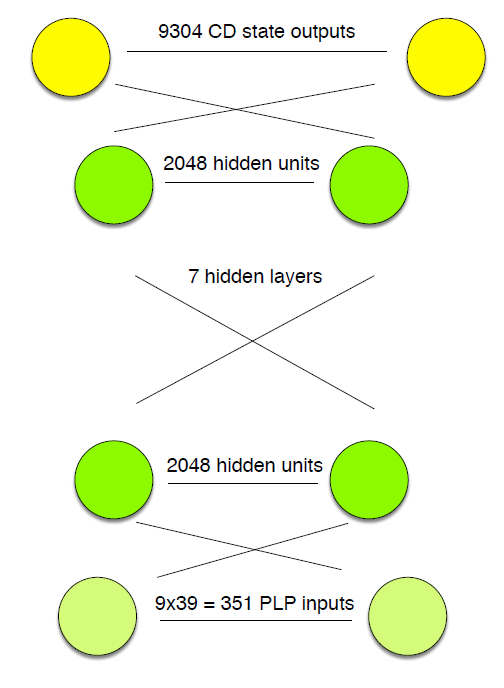
\includegraphics[width=0.5\textwidth]{img/HMMDNN2.png}
    \caption{HMM/DNN acoustic model for Switchboard}
    \label{fig:hmm-dnn-swbd}
\end{figure}

The HMM-DNN acoustic model for Switchboard Corpus\cite{godfrey_switchboard_1992} is depicted in the figure above. Context-dependent HMM/GMM systems are used to generate the alignments. The Viterbi alignment of an HMM/GMM system with 7 hidden layers, 2048 units per layer, and 11 frames of acoustic context yields 9304 output units in our context-dependent Hybrid HMM/DNN system.

When compared to the GMM-based system, the DNN-based system results in a significant reduction in word error rate. DNN/HMM systems model context-dependent tied states with much wider output layers than NN/HMM systems from the 1990s. They can make use of correlated features such as MFCC and FBANK. There is still no speaker adaptation or sequence-level training.

\subsection{Advantages}
\label{sub:hybrid-asr-advantage}

\begin{itemize}
    \item Easily models correlated features. 
    \begin{itemize}
        \item Correlated feature vector components include spectral features.
        \item Input context - multiple frames of data at input.
    \end{itemize}
    \item Greater flexibility than GMMs because it is not made of nearly local components. GMMs are inefficient for non-linear class boundaries.
    \item NNs can simultaneously model multiple events in the input, i.e. different sets of hidden units modelling each event, whereas GMMs assume generation of each from by a single mixture component.
    \item NNs can learn more complex representations and higher-level features such as tandem, posteriorgrams, bottleneck features, and so on.
    \item This method is practical and effective for deployment on Low Computational Resources when compared to Deep Learning Methods and takes less time to train in contrast to Deep Learning Methods.
    \item Maintains the Structure that is required for a Language and Speech Processing System based on which the computer can learn the language. \cite{kincaid_state_2018} Hence this works better in an environment where the context of speech is of the essence. It has also been applied for Continuous Speech Recognition as well. \cite{morgan_continuous_1995} 
    \item When compared to GMM-HMMs, shallow-NN-HMMs, and Multi-layer Perceptrons HMMs (MLPHMMs), the DNN-HMM can extend the labelling ability of GMM-HMM when the hidden layer and hidden unit numbers are set up properly. Thus, DNN-HMMs with discriminative pre-training can produce good results in our scenario as well \cite{li_hybrid_2013}.
\end{itemize}

\subsection{Limitations}
\label{sub:hybrid-asr-limits}

While HMM-DNN continues to produce cutting-edge results, DNN's role is limited. It is primarily used to simulate the posterior state probability of an HMM's hidden state. HMM is still modelling the time-domain feature.

A data alignment problem arises when attempting to model time-domain features with RNN or CNN instead of HMM: both RNN and CNN's loss functions are defined at each point in the sequence, so in order to perform training, the alignment relation between RNN output sequence and target sequence must be known.

Furthermore, GMMs are inefficient for nonlinear class boundaries because they assume each frame is generated by a single component of the mixture. \cite{backstrom_introduction_2022}

\begin{figure}[h!]
    \centering
    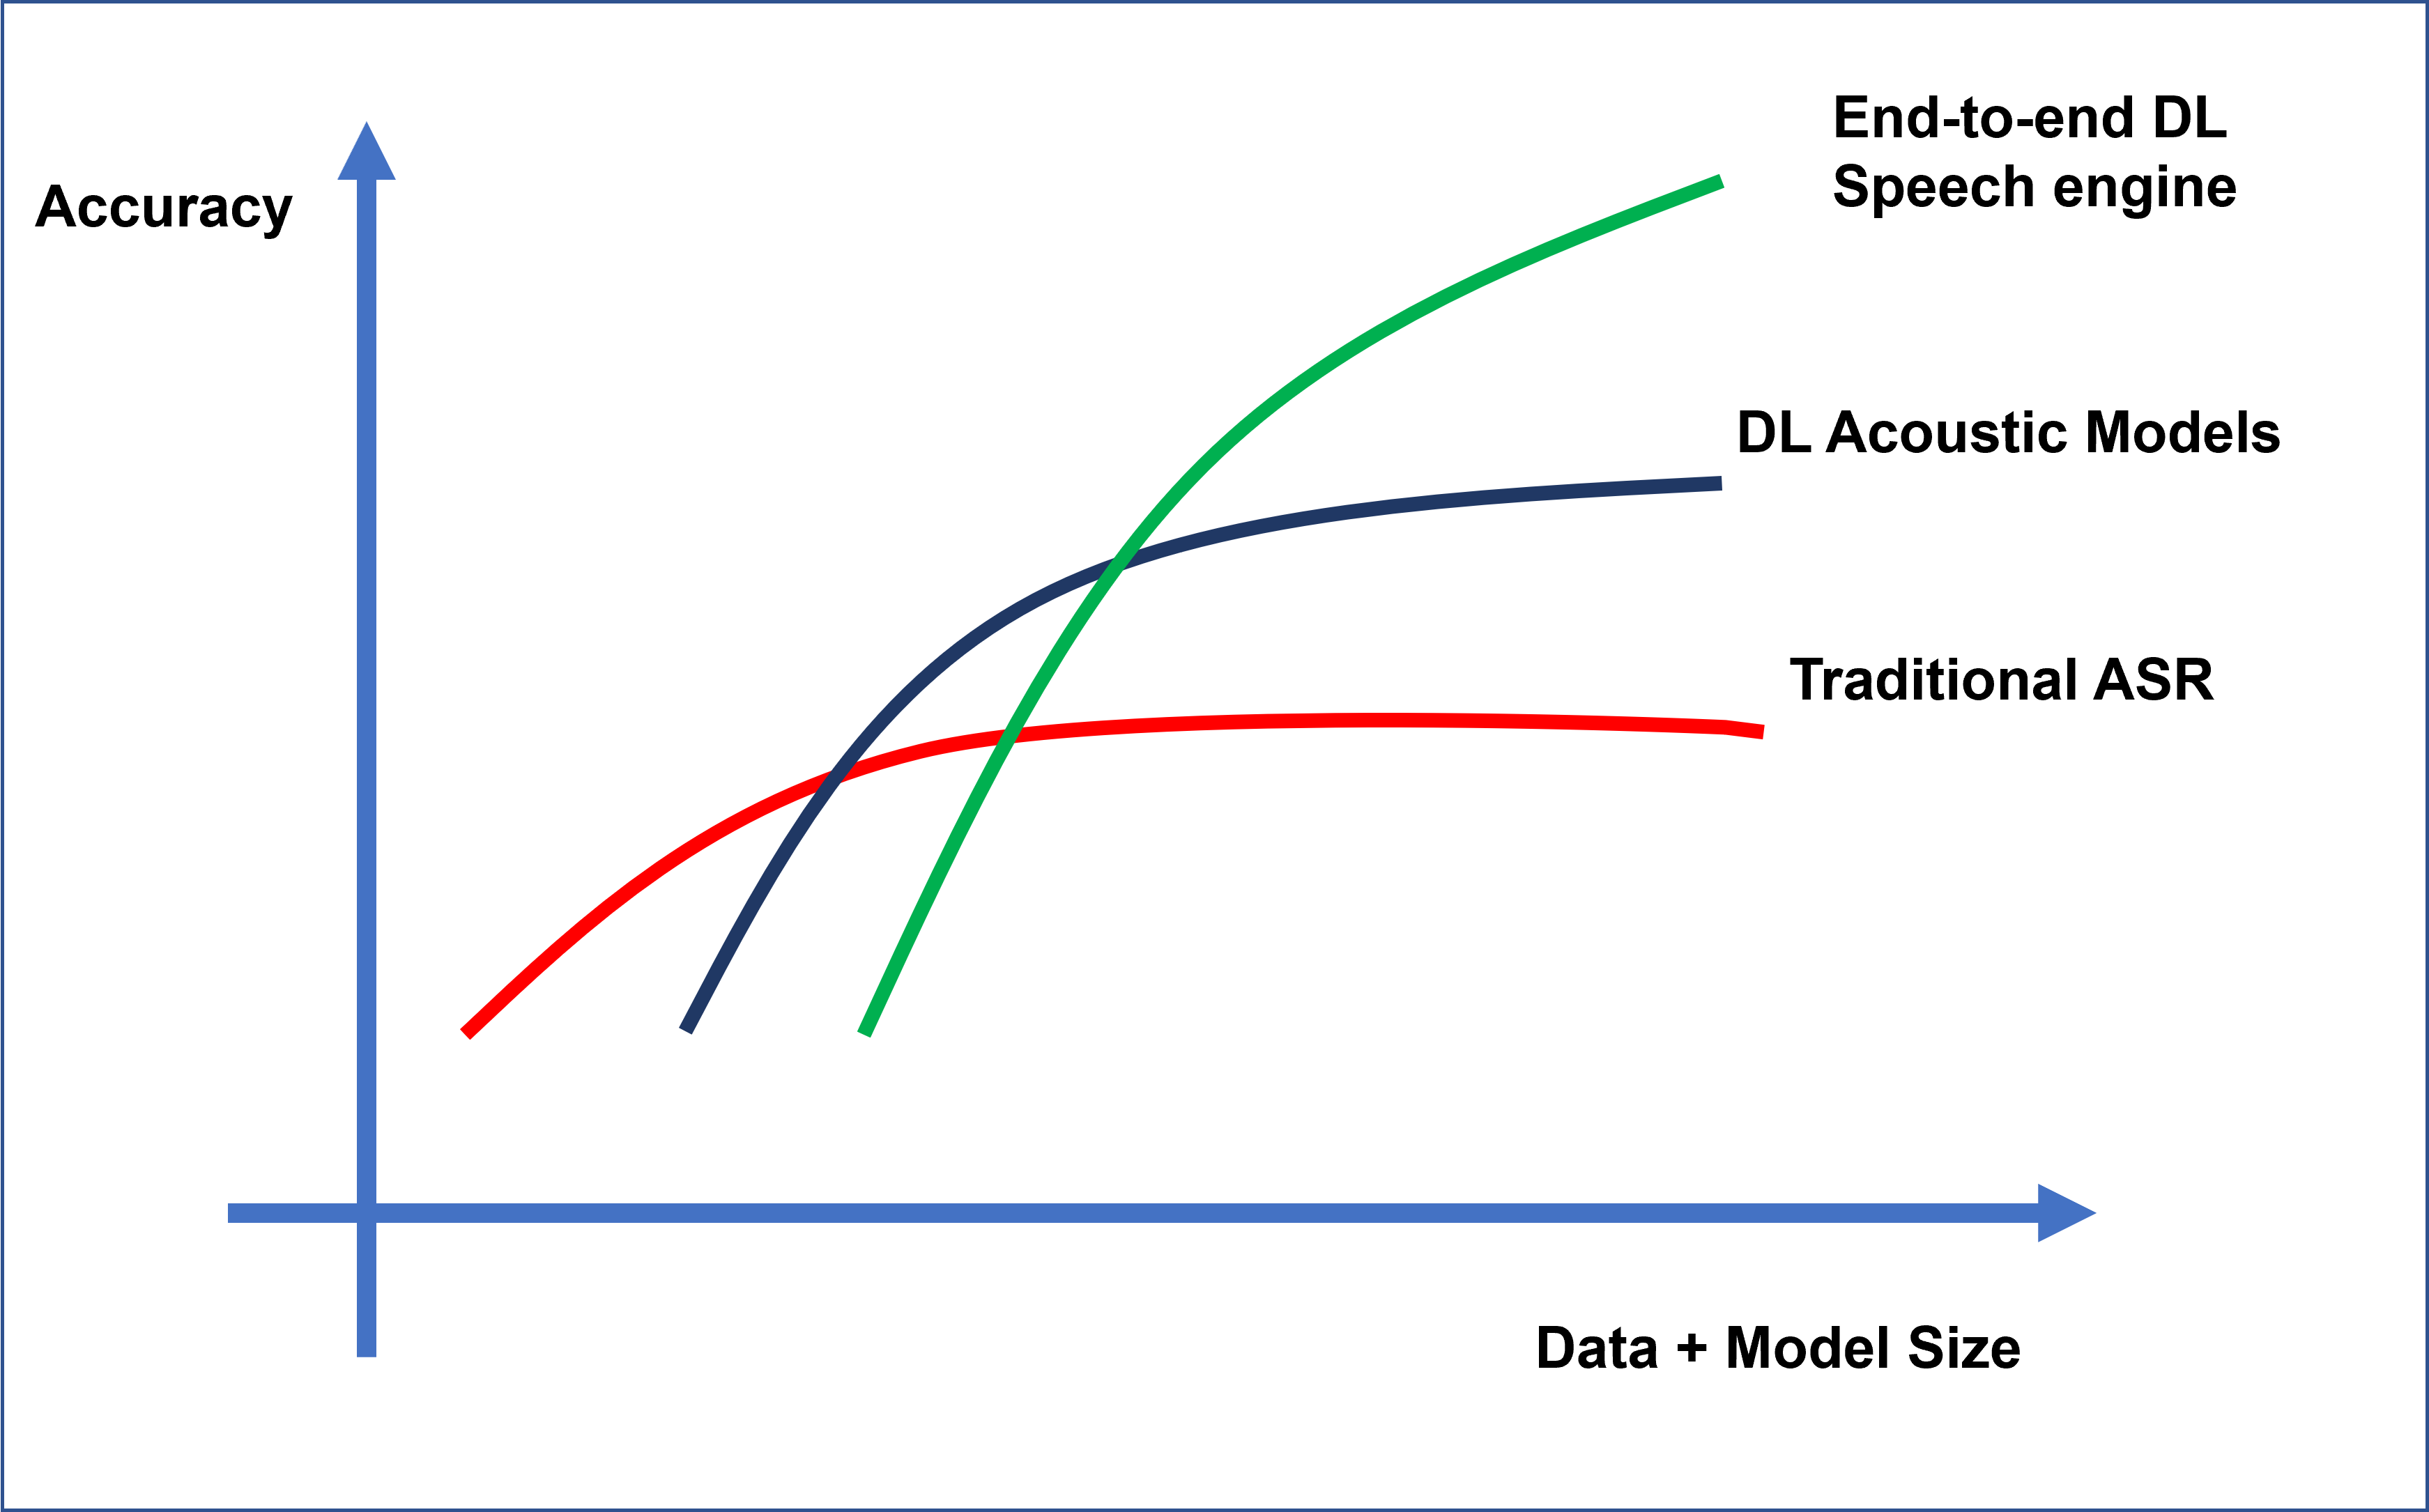
\includegraphics[width=0.7\textwidth]{img/ComparisonASRMODELS.png}
    \caption{Comparison of Three ASR Training Approaches \cite{naeem_subspace_2020}}
    \label{fig:comparison-all-asr-approach}
\end{figure}

\subsection{Choosing our ASR Training Method}
We had huge amount of unlabelled data available. We also had time and budget constrained. There was only one machine available in our Experimental Setup with which we had to build up the ASR. Deep Learning tends to take long time in training which means that errors will be identified after even longer time which makes the process time consuming. 

We decided to take a small set of quality data and train an accurate model on it which will be used to annotate remaining dataset. The data-set will then be audited and improved to build a golden dataset which can then be used to deploy Machine Learning alogrithms to train the most accurate model on a Larger Vocabulary set.

We already had seen \cite{sehar_gul_detecting_2020} work which could not yield optimal performance on small dataset using Deep Learning. Hence, we decided to use Hybrid HMM-DNN method of training ASR which takes relatively less time than Deep Learning while yielding best results.

\cite{georgescu_performance_2021} compared the performance of various ASR engines that use statistical methods and Deep Learning based methods i.e. training data on LibriSpeech (1000hours, 24000 speaker LibriSpeech English data-set) using Kaldi TDNN, CNN-TDNN, Deepspeech2, RWTH RETURNN, FACEBOOK CNN, FACEBOOK TDS, Nvidia Jasper, Nvidia QuartzNet w.r.t Hardware requirements, concluding that Kaldi \cite{daniel_povey_kaldi_nodate} TDNN and CNN-TDNN outperforms its parallels, something supported by previous literature like \cite{christian_gaida_comparing_2014}. 

Another observation was that when compared to TDNN, CNN-TDNN tends to perform slightly better in less clean data-sets (in this case was called test-other data-set) which drew our attention towards using CNN-TDNN for training acoustic model. Many popular Deep Learning-based End to End ASR engines are available like DeepSpeech 2 \cite{amodei_deep_2015-1} but they need a massive amount of labelled data, which is not available in Urdu. 

Therefore, we decided to use CNN-TDNN for training of our Hybrid HMM-DNN ASR. Our long-term approach was to train 10 hours of data to make a strong model and use it to transcribe other audio files to build up our database to 10,000 hours and then apply Deep Learning Models on the golden big data-set.

\section{Speaker Based ASR Model}
\label{sec:spkr-based-asr}

On a speaker's perspective, there are three types of speaker models in ASR:

\begin{enumerate}
    \item \textit{Speaker-independent models} - These models recognise a large number of people's speech patterns. Speaker-independent systems do not require the user to be involved in its development. Any one can use this i.e. they are not specific to any individual. There are various methods for making a system speaker independent:
    \begin{enumerate}[label=(\alph*)]
        \item To capture speaker variation, multiple representations are utilized for each reference.
        \item Approaching to speaker adaptation.
    \end{enumerate}
    \item \textit{Speaker-dependent models} - These models recognise only one person's speech patterns. Both speaker dependent and independent models employ mathematical and statistical formulas to determine the best work match for speech. Speaker-dependent speech recognition systems necessitate user participation in their development. Anyone can use speaker-independent systems. Speaker-dependent systems typically outperform speaker-independent systems because the acoustic differences between speakers are extremely difficult to describe and model. 
    \item \textit{Speaker Adaptive Model} - This is a newly emerging model which begin with a speaker-independent model usually and these models are then adjusted more closely to each individual during a brief period of training.
\end{enumerate}

Our long term aim is to go for Speaker Adaptive model. For our work we will train Speaker Independent model which can later be tuned for Speaker Identification purposes by training it on Speaker Dependent models.


 
\subsection{What are Neural Networks}

An Artificial Neural Network (ANN) is a mathematical model that tries to simulate the structure and functionalities of biological neural networks. Basic building block of every artificial neural network is artificial neuron, that is, a simple mathematical model (function). ANNs are primarily static and symbolic whereas biological neurons are dynamic and analogue.

\subsection{Components of Neural Networks}
Following are key components of Neural Networks:
\begin{itemize}
    \item Neurons: It forms the basic structure of a neural network. When we get the information, we process it and then we generate an output. Similarly, a neuron receives an input, processes it and generates an output which is either sent to other neurons for further processing or it is the final output.
    \item Weights: When an input enters a neuron, it is multiplied by a weight. Initially, the weights are initialized and they are updated during the model training process. When the training is over, the neural network assigns a higher weight value to the input it considers more important as compared to the ones which are considered less important.
    \item Bias: In addition to the weights, another linear component is applied to the input, called as the bias. It is added to the result of weight multiplication to the input. The bias is basically added to change the range of the weight multiplied input.
\end{itemize}

\subsection{Activation Functions}
An activation function in a neural network defines how the weighted sum of the input is transformed into an output from a node or nodes in a layer of the network. Following are types of activation functions in a Neural Network:
\begin{itemize}
    \item Sigmoid - It allows a reduction in extreme or atypical values in valid data without eliminating them: it converts independent variables of almost infinite range into simple probabilities between 0 and 1. Most of its output will be very close to the extremes of 0 or 1.
    \begin{equation}
        sigmoid(x)=\frac{1}{1+e^{-x}}     \end{equation}
    \begin{figure}[h!]
        \centering
        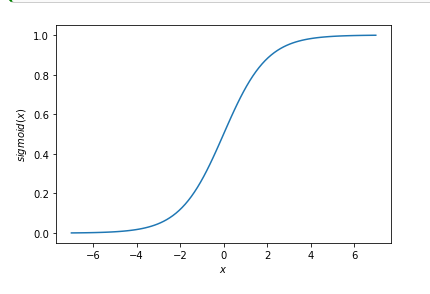
\includegraphics[width=0.5\textwidth]{img/sigmoid.png}
        \caption{Sigmoid Function Graph}
        \label{fig:sigmoid-graphl}
    \end{figure}
    \item ReLU(Rectified Linear Unit) - It has an output of 0 if the input is less than 0, and raw output otherwise. That is, if the input is greater than 0, the output is equal to the input. The operation of ReLU is closer to the way our biological neurons work. 
        
        $$ReLU(x)=max(x,0)$$
        $$=x,x>0$$
        $$=0,otherwise$$
     
    \begin{figure}[h!]
        \centering
        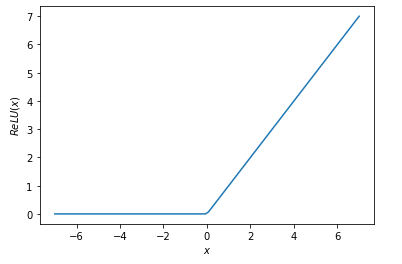
\includegraphics[width=0.5\textwidth]{img/RELU.png}
        \caption{ReLU Graph}
        \label{fig:Relu-graph}
    \end{figure}
    \item Softmax - A modification of the regular max over a vector, such that it has a continuous derivative everywhere. That is, it maps the output to the range [0,1] and simultaneously ensures that the total sum is 1. The output of Softmax is therefore a probability distribution
    $SoftMax(x_{k})=frac{e^{xk}}{\sum_{j=1}{K}e^{xj}}$
    \begin{figure}[h!]
        \centering
        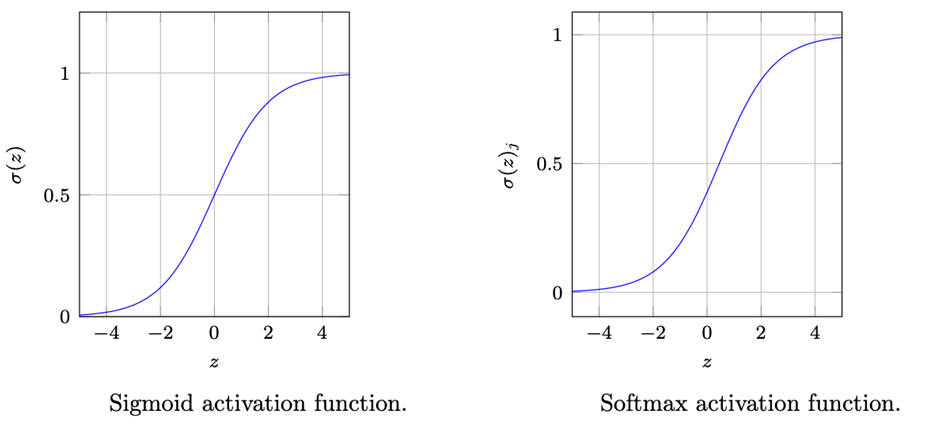
\includegraphics[width=0.9\textwidth]{img/softmax.png}
        \caption{Softmax vs Sigmoid}
        \label{fig:softmax-graph}
    \end{figure}
 
\end{itemize}

\subsection{Parameters of Neural Netowrk}
There are some key parameters of a Neural Network we need to understand:
\begin{itemize}
    \item Input / Output / Hidden Layer : The input layer receives the input and is the first layer of the network. The output layer is the one which generates the output and is the final layer of the network. The processing layers are the hidden layers within the network. These hidden layers are the ones which perform specific tasks on the incoming data and pass on the output generated by them to the next layer. The input and output layers are the ones visible to us, while are the intermediate layers are hidden.
    \item MLP (Multi Layer perceptron): In the simplest network, we would have an input layer, a hidden layer and an output layer. Each layer has multiple neurons and all the neurons in each layer are connected to all the neurons in the next layer. These networks can also be called as fully connected networks.
    \item Cost or loss function: When we train a network, its main objective is to to predict the output as close as possible to the actual value. Hence, the cost/loss function is used to measure this accuracy. The cost or loss function penalizes the network when it makes errors. The main objective while running the network is to increase the prediction accuracy and to reduce the error, thus minimizing the cost function.
    \item Gradient Descent: It is an optimization algorithm used to minimize some function by iteratively moving in the direction of steepest descent as defined by the negative of the gradient.
    \item Learning Rate: The learning rate is a hyper-parameter that controls how much to change the model in response to the estimated error each time the model weights are updated. Choosing the learning rate is challenging as a value too small may result in a long training process that could get stuck, whereas a value too large may result in learning a sub-optimal set of weights too fast or an unstable training process. The learning rate may be the most important hyper-parameter when configuring neural network. Therefore, it is important to know how to investigate the effects of the learning rate on model performance and to build an intuition about the dynamics of the learning rate on model behavior.
    %\item Back-propagation: When we define a neural network, we assign random weights and bias values to our nodes. Once we have received the output for a single iteration, we can calculate the error of the network. This error is then fed back to the network along with the gradient of the cost function to update the weights of the network. These weights are then updated so that the errors in the subsequent iterations is reduced. This updating of weights using the gradient of the cost function is known as back-propagation. In back-propagation the movement of the network is backwards, the error along with the gradient flows back from the out layer through the hidden layers and the weights are updated.
    \item Batches: While training a neural network, instead of sending the entire input in one go, we divide in input into several chunks of equal size randomly. Training the data on batches makes the model more generalized as compared to the model built when the entire data set is fed to the network in one go.
    \item Epochs: An epoch is is a single training iteration of all batches in both forward and back propagation. Thus, 1 epoch is a single forward and backward pass of the entire input data. Although it is highly likely that more number of epochs would show higher accuracy of the network, it would also take longer for the network to converge. You should also take into account that if the number of epochs are too high, the network might over-fit.
    \item Dropout: It is a regularization technique to prevent over-fitting of the network. While training, a number of neurons in the hidden layer are randomly dropped.
    \item Batch Normalization: It normalizes the input layer by adjusting and scaling the activations. For example, if we have features from 0 to 1 and some from 1 to 1000, we should normalize them to speed up learning.
\end{itemize}
\begin{figure}[h!]
    \centering
    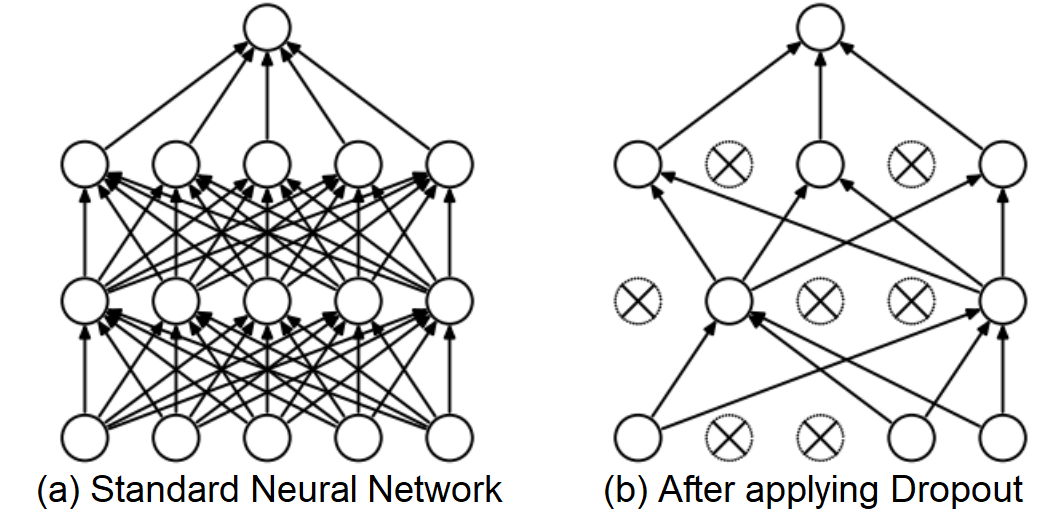
\includegraphics[width=0.9\textwidth]{img/dropout.png}
    \caption{Before and After Dropout}
    \label{fig:droupout}
\end{figure}

\subsection{Propagation in Neural Networks}
Consider a Neural Network containing three inputs $X_{1}$, $X_{2}$ and $X_{3}$, hidden laters with Relu (Rectified Linear unit) activation function which will give zero for any negative value and same value for the positive values the hidden units are $H_{1,2,3,4,5,6}$ then it has the output layer that will be $Y_{1}$ and $Y_{2}$. The neural network also contains biases in our case there are two biases $b_{1}$ and $b_{2}$.

\begin{figure}[h!]
    \centering
    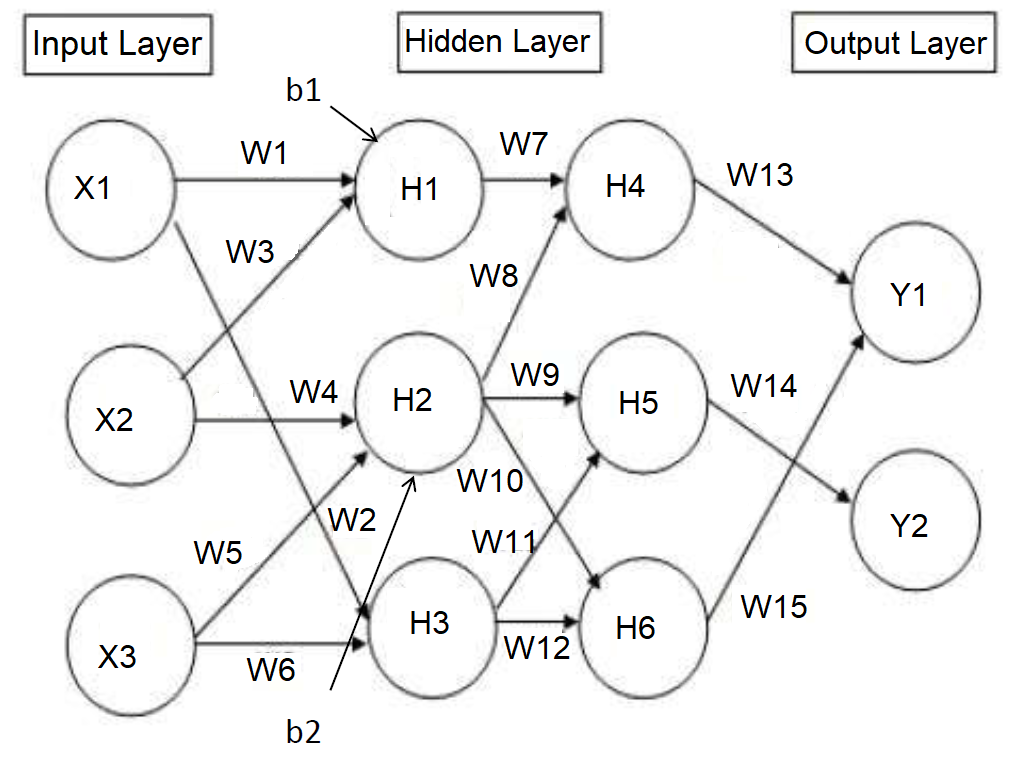
\includegraphics[width=0.7\textwidth]{img/propagation.png}
    \caption{Hidden Layers of NN}
    \label{fig:nn-hiddenlayer}
\end{figure}

\textbf{Forward Propagation:}

It is the way to move from the Input layer (left) to the Output layer (right) in the neural network. In order to achieve the target values we will first perform forward propagation. We will first compute H1 from the following equation;
\begin{equation}
H_{1}=X_{1}*W_{1}+X_{2}*W_{3}+b_{1}    
\end{equation}

where H1 is an activation function, $X_{1}$ is the input, $W_{1}$ is the weight and b1 is the bias. In this way we will calculate $H_{2}$ and $H_{3}$. Next we will calculate $H_{4}$ from the following equation:
\begin{equation}
H_{4}=H_{1}*W_{7}+H_{2}*W_{8}+b_{2}    
\end{equation}

In the same way we will calculate H5, and H6. After calculating all the activation function using input, weights and biases we will then calculate the output $Y_{1}$ and $Y_{2}$ using the following equation respectively:

\begin{equation}
 Y_{1}=H_{4}*W_{13}+H_{6}*W_{15}   
\end{equation}
where Y1 is the first output
\begin{equation}
Y_{2} = H_{4}*W_{14}    
\end{equation}

Once the output is calculated we will then calculate the error as we have set our output target. To compute the error we have the following equation:

\begin{equation}
\Xi E_{Total} = \Xi (0.5)(target - output)^2    
\end{equation}

In order to reduce this loss, we will update our weights and for that, we will have to perform backward propagation.

\textbf{Backward Propagation:}
The process of moving from the right to left i.e backward from the Output to the Input layer is called Backward Propagation.

In the Back Propagation weights are updated so as to achieve the target values and to minimize the loss that is calculated by subtracting the output target to the actual target. We will first update the weights of W13 for that we have the following equations
\begin{equation}
\frac{\delta E_{Total}}{\delta W 13} = \frac{\delta E_{Total}}{\delta_{out} Y1} \frac{\delta_{out}Y1}{\delta Y1}  \frac{\delta Y1}{\delta W13}     
\end{equation}
 
Now we calculated update W13
\begin{equation}
W_{13(Updated)} = W13-\eta \frac{\delta E_{total}}{\delta W13}    
\end{equation}

We will update $W_{14 and 15}$ in this way as well.

Now to second hidden layer to update weights.

\begin{equation}
    \frac{\detla E_{Total}}{\delta W_{7}} = \frac{\delta E_{total}}{\delta_{out} H_{4}}.\frac{\delta_{out} H_{4}}{\delta J_{4}}.\frac{\delta H_{4}}{W_{7}}
\end{equation}

Now updating the weights
\begin{equation}
    W_{7(Updated)} = W_{7} = \eta . \frac{\delta E_{total}}{\delta W+{7}}
\end{equation}

In this way we will update the weights of $W_{8,9,10,11,12}$. Now we will move to the next layer and will update the weights:

\begin{equation}
\frac{\delta E_{Total}}{\delta W_{1}} = \frac{\delta E_{total}}{\delta_{out}H_{1}}*\frac{\delta_{out}H_{1}}{\delta H_{1}}*\frac{\delta H_{1}}{\delta W_{1}}    
\end{equation}

Updating the weights we get:
\begin{equation}
W_{1(Updated)} = W_{1}-\eta*\frac{\delta E_{total}}{\delta W_{1}}    
\end{equation}

In this way we will update the weights of W2, W3, W4 and W5 Once all the weights are updated we will then perform forward propagation with the newly updated weights this will reduce our error as we will reach near our targeted value the forward and backward propagation will be repeated again and again until we will achieve our target value.

\subsection{Deep Neural Networks (DNNs)}
Deep Neural Network (DNNs) are an artificial neural network (ANN) with multiple layers between the input and output layers unlike Shallow Neural Network which has only one layer. Many experts define deep neural networks as networks that have an input layer, an output layer and at least one hidden layer in between. Each layer performs specific types of sorting and ordering in a process that some refer to as “feature hierarchy.” One of the key uses of these sophisticated neural networks is dealing with unlabeled or unstructured data. The phrase “deep learning” is also used to describe these deep neural networks, as deep learning represents a specific form of machine learning where technologies using aspects of artificial intelligence seek to classify and order information in ways that go beyond simple input/output protocols.

\begin{figure}[h!]
    \centering
    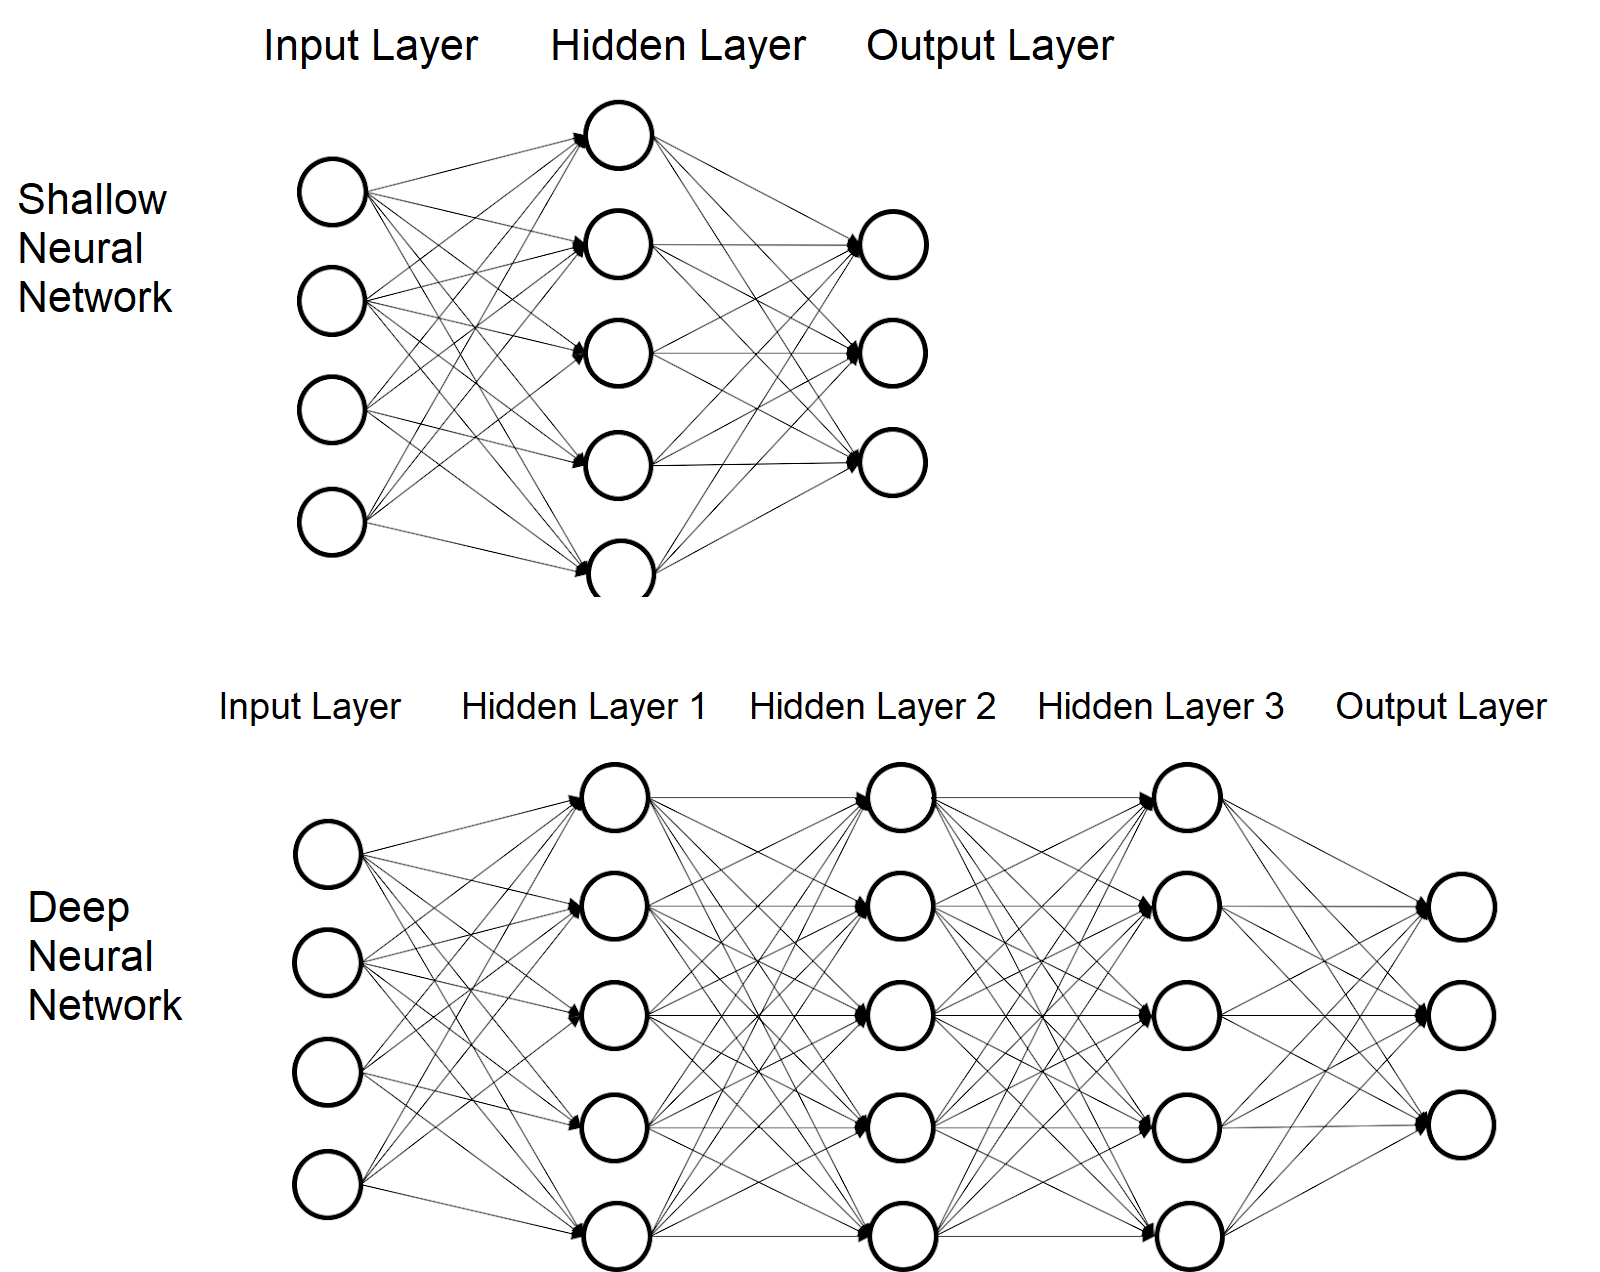
\includegraphics[width=0.7\textwidth]{img/DNN.png}
    \caption{Shallow vs Deep Neural Networks}
    \label{fig:shallow-deep-NN}
\end{figure}

\subsection{Convolutional Neural Networks}
\label{sub:CNN}
This was first proposed by \cite{fukushima_neocognitron_1988} and used by \cite{lecun_gradient-based_1998}. It is very popular for image classification but is also used in Speech technology\cite{abdel-hamid_exploring_2013} \cite{ghahremani_acoustic_2016} \cite{dua_developing_2022}. The advantages of CNNs over DNNs include CNNs are highly optimized for processing 2D and 3D images, and are effective to learn and extract abstractions of 2D features. In addition to these, CNNs have significantly fewer parameters than a fully connected network of similar size.

CNNs consist mainly of two parts: feature extractors and classifier. In the feature extraction module, each layer of the network receives the output from its immediate previous layer as its input and passes its output as the input to the next layer. The CNN architecture mainly consists of three types of layers: convolution, pooling, and classification.

\begin{figure}[h!]
    \centering
    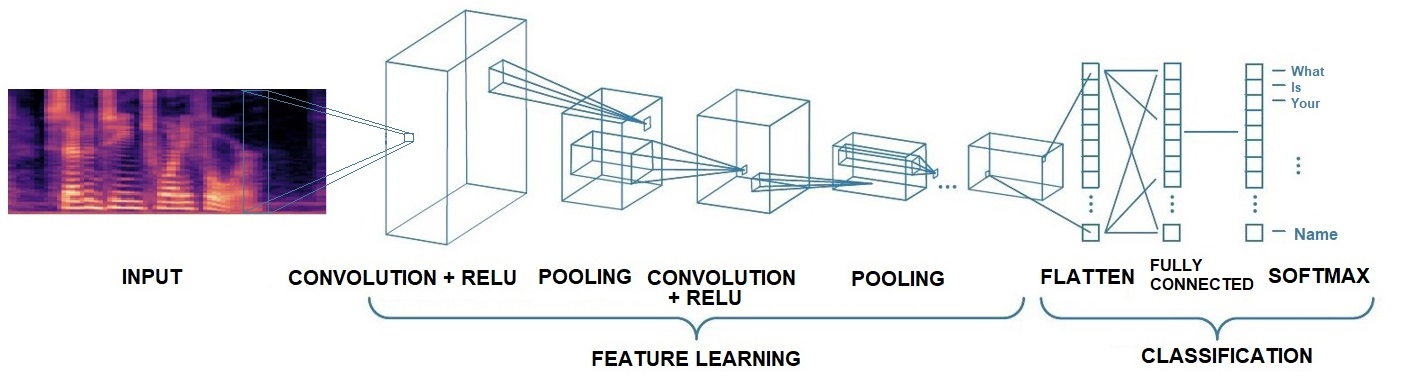
\includegraphics[width=0.8\textwidth]{img/CNN.jpg}
    \caption{CNN Architecture}
    \label{fig:cnn-arch}
\end{figure}

The main layers in Convolutional Neural Networks are:
\begin{enumerate}
    \item Convolutional layer: A “filter” passes over the image, scanning a few pixels at a time and creating a feature map that predicts the class to which each feature belongs. Thus, in this layer, feature maps from previous layers are convolved with learnable kernels. The output of the kernels goes through a linear or non-linear activation function, such as sigmoid, hyperbolic tangent, Softmax, rectified linear, and identity functions) to form the output feature maps. Each of the output feature maps can be combined with more than one input feature map.
    \item Pooling layer: It reduces the amount of information in each feature obtained in the convolutional layer while maintaining the most important information (there are usually several rounds of convolution and pooling).
    \item Fully connected input layer (flatten): It takes the output of the previous layers, “flattens” them, and turns them into a single vector that can be an input for the next stage.
    \item The first fully connected layer: It takes the inputs from the feature analysis and applies weights to predict the correct label
    \item Fully connected output layer: It gives the final probabilities for each label
\end{enumerate}

Higher-level features are derived from features propagated from lower-level layers. As the features propagate to the highest layer or level, the dimensions of features are reduced based on the size of the kernel for the convolution and pooling operations respectively. However, the number of feature maps usually increases for representing better features of the input images for ensuring classification accuracy. The output of the last layer of the CNN is used as the input to a fully connected network. Feed-forward neural networks are used as the classification layer since they provide better performance.

\subsection{TDNN}
\textbf{Time-Delay Neural Network (TDNN)} is a time-domain convolutional network that models temporal dependencies. This is easier to parallelize than a recurrent network and, in terms of training time, is comparable to feed-forward DNN. Each unit's input in TDNN layers is spatially expanded out in a couple of sequential units from the previous layer. Hence, the lower layers learn a narrower context while the higher layers process activations for a broader temporal context. The lengths of each layer's input context represent the hyper-parameters for a TDNN \cite{kreyssig_improved_2018}.

TDNN employs a sub-sampling technique to compute hidden activations only at specific time steps which avoids redundancy because the large overlap of contexts leads to highly correlated neighbouring activations. A larger context on the left side was found to be optimal for online decoding. Both, Model size and training time are reduced \cite{georgescu_performance_2021}.

Hence, the TDNN network's sub-sampling mechanism is similar to a convolutional operation that allows gaps in the convolutional filter. This is another network variant based on the purely TDNN approach, with a couple of stacked convolutional layers added before. Their primary function is to process the acoustic features further and act as a feature processing front-end. These additional layers reduce spectral and temporal variability. Convolutional layers have the property of annihilating small variations in the spectral domain due to their structure provided by local connectivity, weight sharing, and pooling \cite{georgescu_performance_2021}.

These variations are induced by both the speaker and the acoustic environment in which the speech takes place. Various reports like \cite{abdel-hamid_convolutional_2014}, \cite{zorila_investigation_2019}, \cite{biswas_semi-supervised_2019}, \cite{noauthor_tdnn_nodate} and \cite{kreyssig_improved_2018} suggest that CNN-TDNN perform better than simple TDNN, however, the former requires relatively a bit more computing power \cite{georgescu_performance_2021}.

\subsection{CNN-TDNN}

Ghahremani \cite{ghahremani_acoustic_2016} proposed a CNN-TDNN-based raw waveform setup with a repeated network-in-network structure that aggregates time information from convolution filter outputs. If this NIN non-linearity replaces the conventional ReLU hidden layer in the DNN, the results improve. 

\textbf{CNN-TDNN} is a variant of simple TDNN model, which was initially implemented in the Kaldi toolkit on the LibriSpeech task. It is part of a multi-component system comprising of a hybrid TDNN-HMM based acoustic model, a phonetic model and an n-gram language model. 

Similarly, a complex n-gram or neural network based language model can be used optionally for re-scoring. Mel-filter-banks are used in this implementation instead of MFCCs, in terms of network input features. Unlike the previous case of simple TDNN where the input features are represented as a vector, final features are organized as a matrix. The input in the CNN-TDNN network is composed of two types of features which are organized in a 40x6 matrix of speech features (Feature type no. 2) \cite{georgescu_performance_2021}: 
\begin{enumerate}
    \item 40-dimensional Mel-filter-banks extracted from 25 ms length frames
    \item 200-dimensional and 10 ms shift i-vectors calculated from chunks of 150 consecutive frames
\end{enumerate}

The feature extraction procedure and organization of these features are shown in Figure \ref{fig:CNNTDNNvsTDNNl} on the central part of the left column.

The acoustic model's neural network component is quite similar to the previous TDNN network, with the main difference being a few CNN layers placed before the time-delay layers, which act as a front-end block. As input for the Conv. Block 1, three matrices of speech features (Feature Type no. 2) are provided: the features for the current, previous, and next acoustic frames, or, equivalently, a feature volume of 6 x 40 x 3. Time and feature space convolutions are performed using 64 filters of size 3x3, and a 64 x 40 x 1 volume is the output \cite{georgescu_performance_2021}.

CNN blocks with front end role are followed by twelve blocks of factored TDNN i.e. TDNN-F. The first TDNNF i.e. TDNN-F Block 1, only processes the current time frame, whereas the rest perform temporal convolution over the time indexes $t-3$, $t$, and $t+3$. The input vectors at time indexes $t-3$ and $t$ are spliced together to form the linear layer, while the input vectors at time indexes $t$ and $t+3$ are spliced together to form the affine layer \cite{abdel-hamid_convolutional_2014}. Figure \ref{fig:CNNTDNNvsTDNNl} depicts the entire CNN-TDNN network in the central column.  

The NN output blocks of the CNN-TDNN and simple TDNN architecture are identical which is represented by 6016-dimensional posterior probabilities of the acoustic states, while the output of the system is given by the 200k words language model. 

The Convolution Block 2 input is comprised of three time consecutive volumes as the Convolution Block 1 output, which are spliced together to form the 64 x 40 x 3 feature volume. The second convolutional block performs time and feature space convolutions with another 64 3x3 filters and outputs a 64 x 40 x 1 volume.

%The input of the Conv. Block 2 consists of three time consecutive volumes as the one output by Conv. Block 1, which are spliced together to form the 64 x 40 x 3 feature volume. The second convolutional block applies another 64 filters of size 3x3 to perform time and feature space convolutions and outputs a 64 x 40 x 1 volume. More filters are applied in Conv. Blocks 3 to 6, from 128 up to 256, while the size of the feature volume is kept constant by decreasing the height from 40 to 20 and finally to 10. The convolutional blocks are providing a 2560-dimensional output which is passed to the succeeding time-delay blocks.

More filters are used in Conv. Blocks 3–6, ranging from 128 to 256, while the size of the feature volume is maintained by decreasing the height from 40 to 20, and finally to 10. The convolutional blocks generate a 2560-dimensional output that is passed on to the following time-delay blocks \cite{georgescu_performance_2021}.

\newpage
\begin{landscape}
  \begin{figure}[h]
    \centering
    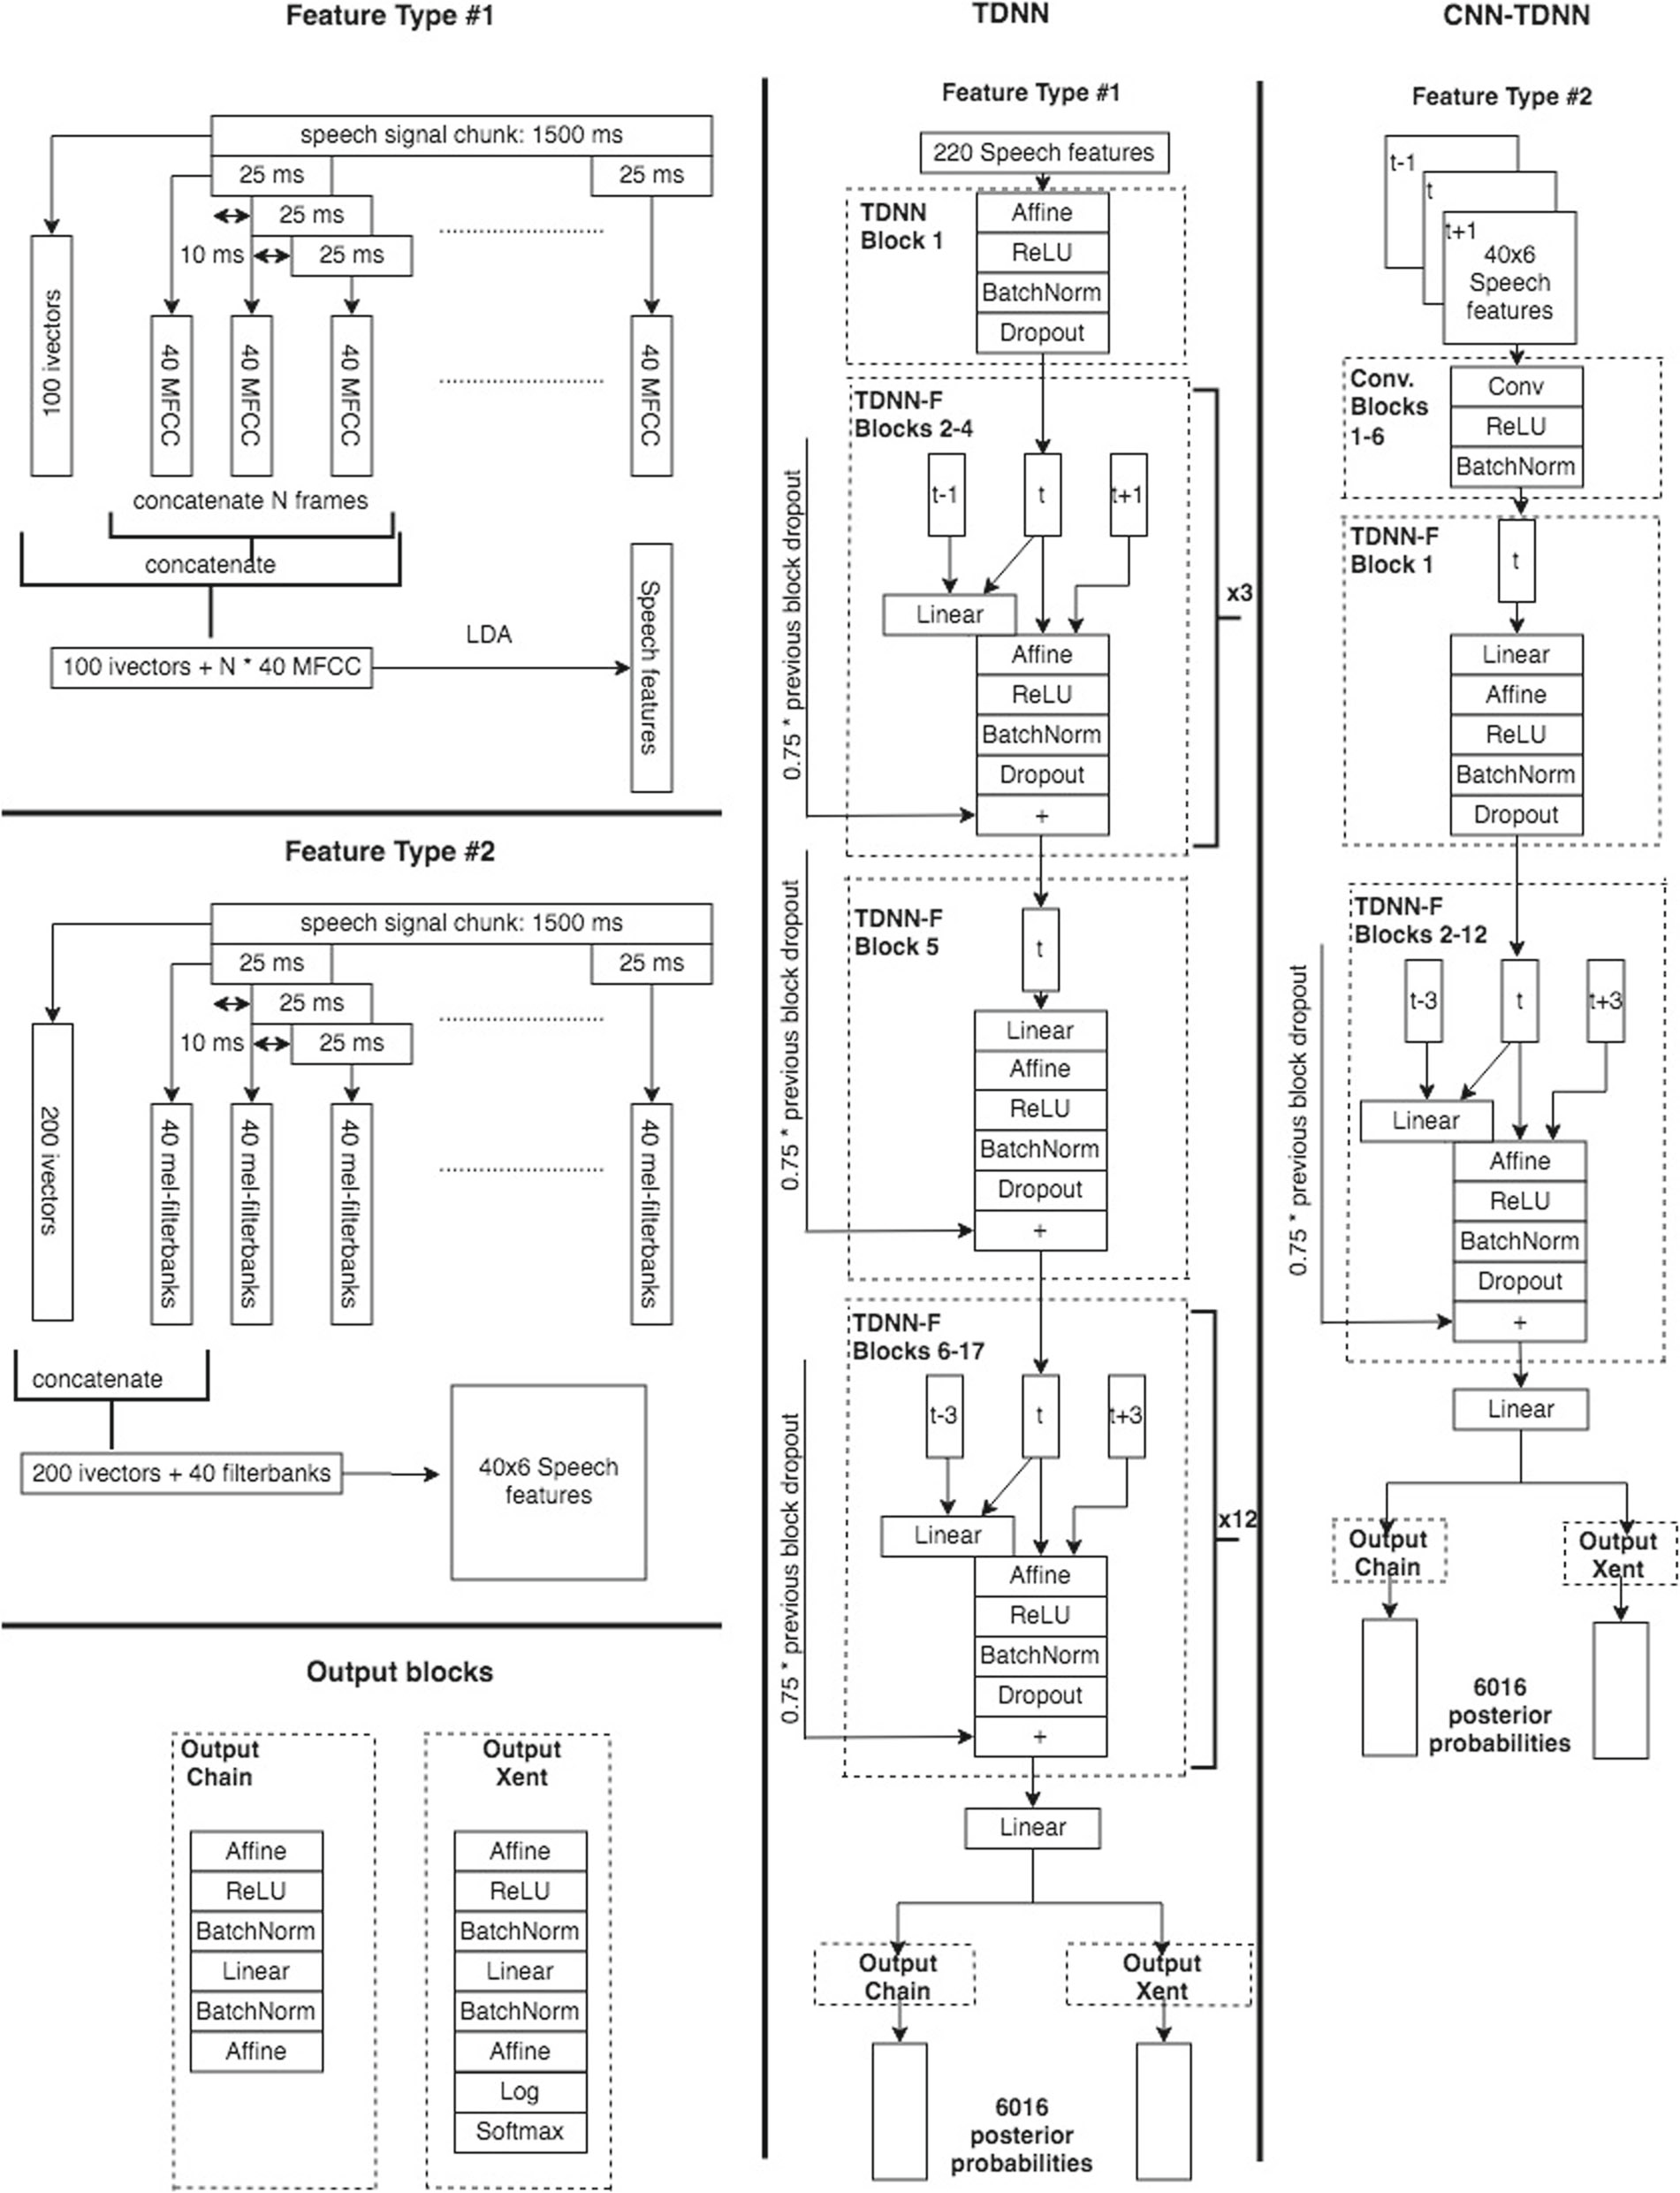
\includegraphics[width=1.0\textwidth, angle=90]{img/TDNNvsCNNTDNN.png}
    \caption{Feature types and architectures TDNN and Chain CNN-TDNN \cite{georgescu_performance_2021}}
    \label{fig:CNNTDNNvsTDNNl}
  \end{figure}  
\end{landscape}
\newpage

In Figure \ref{fig:CNNTDNNvsTDNNl}, feature type no. 1 (upper left) is used in TDNN models (center) and feature type 2 (middle left) is used in CNN-TDNN models (right). The output blocks (bottom left) that use cross-entropy and chain loss functions are used in both architectures.

%The performance was investigated by \cite{georgescu_performance_2021}, which shows that it performed very close to TDNN in a clean data-set of Librispeech but on "other" data-set of LibriSpeech, it actually performed better. 


\section{Challenges} % (fold)
\label{sec:challenges}

Our literature review shows that although work has been done on the field in general, there is little applicable research that can be put in production environment for our use a noisy telephonic environment. 

Following challenges need to be addressed in this regards:

\begin{itemize}
    \item Lack of availability of accurate models for Code-Switched urdu Language for noisy telephonic environment. Code-switching which is very common in low-resource languages like Urdu is hard to model if only monolingual training data is available. It can interpolate monolingual language models, but likely switching points may not be easy to predict. We will also need to consider if there is a change in phonology. 
    \item Collection of Diverse dataset in terms of:
    \begin{itemize}
    \item Isolated Digits
    \item Isolated words
    \item Read Speech (Words and Digits)
    \item Spontaneous Speech (Words and Digits)
    \item Clean Audio
    \item Noisy or Telephonic Audio
    \end{itemize}
    \item Limited availability of dataset is a major challenge in ASR implementation \cite{pironkov_hybrid-task_2020}, \cite{wang_wavenet_2020}. \item The open-source data-set available online are very limited and cannot be used to train accurate ASR and not much has been done for training accurate ASR on low-resourced languages.
    \item Sharing of data by organizations puts up many questions regarding privacy (see \ref{sub:security_privacy_asr_research})
    \item Very less research on development of code-switched Urdu ASR in Noisy or Telephonic environment. Noise reduces ASR performance \cite{lee_dnn-based_2016} since acoustical features will suffer greatly, particularly in short-frame detection \cite{ming_speech_2017}.
    \item Spontaneous Speech in telephonic conversation has Pronunciation issues e.g. due to medical issue or children speech, which reduces ASR performance \cite{kumar_leveraging_2020}.
    \item Noise signals in practical situations has a variety of properties\cite{lee_threshold-based_2018} and due to this diversity, creating a database that responds to external noise is a significant challenge for DNN-based systems \cite{gosztolya_domain_2016}.
    \item Noisy environments contribute to the absence of spectro-temporal information in input signals, resulting in missed time-frequency correlations of the underlying speech signal \cite{ganapathy_multivariate_2017}. Despite the fact that many noise reduction methods have been developed, these methods are ineffective unless the noise sources are known.
\end{itemize}



The chain model is same as standard DNN-HMM with currently a threefold reduced frame rate at the DNN's output. The DNN's input features are at the original frame rate of 100 frames per second because all of the CNNs, LSTMs, TDNNs etc have a type of recurrent connections or splicing inside them, indicating that they are not purely feed-forward nets.

%Kaldi uses TDNNs as the neural net because they are easier to tune than LSTMs, and gives a better WER than the baseline TDNN: 11.4%, versus 12.1% for the best TDNN baseline (on the Switchboard-only portion of eval2000).

This model has a different objective function used for its training i.e. instead of a frame-level objective, log-probability of the correct phone sequence is used. 

%In principle, the training process is very similar to MMI training in that we compute numerator and denominator 'occupation probabilities' and use the difference between the two in the derivative computation. 

It is no longer necessary to normalise the DNN outputs to sum to one on each frame; such normalisation makes no difference. We must use a modified HMM topology due to the reduced frame rate (one frame every 30 ms). 

We want the HMM to be traversable in a single transition (as opposed to the 3 transitions of a model mat the normal frame rate). The currently preferred topology has a state that can only appear once, followed by another that can appear zero or more times. The state-clustering is obtained in the same manner as for GMM-based models, albeit with a different topology (we convert the alignments to the new topology and frame-rate).

The training procedure for chain models is a lattice-free version of MMI, in which the denominator state posteriors are obtained by a forward-backward algorithm over an HMM formed from a phone-level decoding graph, and the numerator state posteriors are obtained by a similar forward-backward algorithm but limited to transcript-corresponding sequences.

A derivative of the form (numerator occupation probability - denominator occupation probability) for each neural net output index (i.e. for each pdf-id) is computed and these are propagated back to the network.

\textbf{The denominator FST:}

We do forward-backward over an HMM for the denominator part of the computation. Actually, because we represent it as a finite state acceptor, the labels (pdf-ids) are associated with the arcs rather than the states, so it's not a true HMM in the traditional sense, but it's easier to think of it as an HMM because we use the forward-backward algorithm to obtain posteriors. %We refer to it as the 'denominator FST' in the code and scripts.

\textbf{Phone language model for the denominator FST:}

The first step in building the denominator FST is to develop a phone language model. This language model is derived from phone alignments in training data. This is an un-smoothed language model, which means we never revert to lower order n-grams. %Some language-model states, however, are completely removed, so transitions to those states instead go to the lower-order n-state gram's. We avoid smoothing in order to reduce the number of arcs in the compiled graph after phonetic context expansion.

A 2- phone history is always required to be maintained and hence a 4-gram language model is used and we never prune LM states below the trigram level. The reason for not pruning the trigrams is that any sparsity in which trigrams are permitted tends to reduce the size of the compiled graph. %In addition to the number of states dictated by the no-prune trigram rule, we have a selectable number (e.g., 2000) of 4-gram language model states to be retained (the rest are identified with the corresponding trigram state), and the ones we select are determined in a way that maximises the training-data likelihood. To maximise the training-data likelihood, all probabilities are estimated. 

%It is worth noting that if our phone LM was just a simple phone loop (i.e. a unigram), it would be expanded to triphones due to phonetic context effects, but it would contain arcs for all possible trigrams. So any sparsity obtained by using the un-pruned trigram model is a bonus. Empirically, an un-smoothed trigram LM is what expands to the smallest possible FST; and pruning some of the trigrams results in little or no WER improvement while increasing the size of the compiled FST (at least on 300 hours of data expanded 3-fold with speed perturbation; on less data it might help).

%The phone-LM perplexities for the various models we tried on the Switchboard setups ranged from 5 to 7; the phone-LM perplexity with our chosen configuration (4-gram, pruned to trigram for all but 2000 states) was around 6. Lower phone-LM perplexity did not always result in better WER of the trained system; for conventional (word-based) MMI training, an intermediate strength of language model seemed to work best.

\textbf{Compilation of the denominator FST:} 

The phone language model is expanded into an FST with 'pdf-ids' as the arcs, in a process similar to decoding-graph compilation in normal Kaldi decoding, except that no lexicon is involved, and we convert the transition-ids to pdf-ids at the end.

One distinction is in graph size minimization. The standard recipe calls for determinization and minimization. This procedure, or variants of it with disambiguation symbols, did not allow us to reduce the size of the graph. Instead, our graph-minimization procedure can be summarised as "repeat three times: push, minimise, reverse; push, minimise reverse." The terms 'push' and'reverse' refer to reversing the directions of arcs and swapping initial and final states.

\textbf{Initial \& Final Probabilities \& Normalization FST:}

The graph-creation process discussed above naturally produces an initial state and final probabilities for each state; however, these are not the ones we use in the forward-backward procedure because these probabilities apply to utterance boundaries, but we train on fixed-length chunks of utterance (e.g. 1.5 seconds). Constraining the HMM to the initial and final states at these arbitrarily chosen cut points is not appropriate. Instead, we use initial probabilities derived from a fixed number of iterations of 'running the HMM' and averaging the probabilities; and final probabilities equal to 1.0 for each state.

%We have an explanation but don't have time to explain it right now. As part of the computation in the denominator forward-backward process, we apply these initial and final probabilities to the initial and final frame. However, we can also write a version of the denominator FST with these initial and final probabilities, which we call the 'normalisation FST.' (Because FSTs do not support initial probabilities, epsilon arcs are used to simulate them.) This'normalization FST' will be used to add probabilities to the numerator FSTs in a manner that will be explained later.

\textbf{Numerator FSTs:}

Numerator FST is created for each utterance for preparation of the training process which encodes the supervision transcript as well as an alignment of that transcript i.e., it forces similarity to a reference alignment obtained from a baseline system, but allows for some room to differ from that reference. 

In the lattice alignment, a phone is allowed to occur 0.05 seconds before or after its begin and end positions, respectively. Incorporating alignment information is important because we train on fixed-length pieces of utterances rather than entire utterances i.e. splitting up the utterance into pieces if we know where the transcript aligns. %(which is important for GPU-based training)

Instead of enforcing a specific pronunciation of the training data, we use a lattice of alternative pronunciations of the training data generated by a lattice-generating decoding procedure using an utterance-specific graph as the decoding graph as our reference. This generates all pronunciation alignments that were within a beam of the highest-scoring pronunciation.

\textbf{Splitting the numerator FST:s}

Fixed sized utterances (e.g. 1.5 seconds in length) are used which necessitates division of the numerator FSTs into fixed-size pieces which is simple because the numerator FSTs, which remember and encode time-alignment information, have a structure that allows association of any FST state with a specific frame index. %At this point, there are no costs in the numerator FST — just it's viewed as encoding a constraint on paths — so there is no need to decide how to split up the costs on the paths.

\textbf{Normalizing the numerator FSTs:}

To ensure that the costs from the denominator FST are reflected in the numerator FST, split-up pieces of numerator FST with 'normalisation FST' are combined which ensures that objective functions can never be positive, making them easier to interpret. It also protects against the possibility that the numerator FST contains state sequences that the denominator FST does not allow, which could allow the objective function to increase indefinitely.

%Because the phone LM lacks smoothing and is estimated from 1-best alignments, the lattices may contain phone n-gram sequences that were not seen in training.

%This normalisation process occasionally (but infrequently) generates an empty FST: this can happen when the lattice contains triphones that were not present in the 1-best alignment used to train the phone language model, and there are no alternative paths at that point in the lattice that could compensate for the resulting 'failed' paths. This is possible because the 1-best alignment and the lattice-producing alignment selected different pronunciations of the same word. These utterance fragments are simply discarded.

\textbf{Format of the numerator FSTs:}

The weighted acceptors in the numerator FSTs correspond to pdf-ids plus one. Pdf-ids can not be used because they could be zero which is treated differently by OpenFst (as epsilon). 

Instead of storing an array of separate numerator FSTs, we append them together to form a longer FST when we form minibatches, allowing us to do a single forward-backward over all utterances in the minibatch, which directly computes the total numerator log-probability. %(This isn't a significant feature; it's simply a software detail that we explain here to avoid confusion.)

\textbf{Fixed-length Chunks \& Minibatches:}

Utterances were divided into fixed-length chunks of speech to train on minibatches of length 1.0 seconds in our current scripts. Utterances shorter than this are discarded; those longer are divided into chunks with either overlaps or small gaps between them. We used Frames per e.g = 150, 110, 100, 30 due to varying size of our dataset and 10 Epochs and Initial Number of jobs =3 and Final Number of jobs= 16 for trainer optimization.  

%It's worth noting that our acoustic models typically require left or right frames for acoustic context; we add that, but it's a separate issue; the context is added after the chunks have been determined.

Minibatch size is usually a power of two, and it can be constrained by GPU memory constraints. We used 64 mini-batches based on our dataset. The alpha probabilities in forward-backward computation are the largest single consumer of GPU memory. After the 3-fold sub-sampling, we have 50 time steps with a 1 second chunk. 

%A typical denominator FST in our Switchboard setup has 30,000 states. For the alphas, we use single-precision floating point, so the memory used in gigabytes is (128 * 50 * 30000 * 4) / 109 = 0.768G.

%This will not consume all of the GPU memory, but there are other sources of memory, for example, we keep around two copies of the nnet outputs in memory, which takes a fair amount of memory depending on the configuration- for example, replace the 30000 above with around 10000 to get the amount of memory used for one copy of the nnet outputs in a reasonable configuration.

%\textbf{Training on frame-shifted data}
%There are methods available for generating perturbed data in neural net training to artificially increase the amount of data we train on. To create 3-fold augmented data, our standard nnet3 neural-net training example scripts time-warp the raw audio by factors of 0.9, 1.0, and 1.0. This is orthogonal to the 'chain' models, and we do it (or do not do it) in the same way that we would for the baseline. However, we can supplement the data for the chain models in another way by shifting the frames.

%Because we only evaluate nnet output at t values that are multiples of 3, we can generate different versions of the training data by shifting the training examples by 0, 1, and 2 frames.

%This is done automatically in the training script and 'on the fly' as we read the training examples from disk- the programme nnet3-chain-copy-egs has a -frame-shift option that the script sets. 

%This has an impact on how the number of epochs is interpreted. If the user requests 4 epochs, for example, we actually train for 12 epochs; we just do so on three different-shifted versions of the data. The -frame-shift=t option actually shifts the input frames by t and the output frames by the closest multiple of 3 to t. (In general, it may not be 3, but it is a configuration variable called -frame-subsampling-factor.)

%\textbf{GPU issues in training}
%The forward-backward over the numerator FST and over the denominator HMM computations are unique to the 'chain' computation. The numerator of this is extremely fast. Because there can be a lot of arcs in the denominator FST, the denominator forward-backward takes a long time (e.g. 200,000 arcs and 30,000 states in a typical Switchboard setup). The time required can be nearly as long as the time required in the neural-net parts of the computation. We took great care to ensure memory locality.

%The next step, most likely, will be to implement a pruned version of the forward-backward computation (like pruned Viterbi, but computing posteriors). To get a speedup, we'd have to remove a large number of states in order to compensate for the loss of memory locality that pruning would cause.

%We are careful in our current implementation to ensure that a group of GPU threads are all processing the same HMM-state and time, but from different chunks (we call these different'sequences' in the code); and we make sure that the memory locations corresponding to these different sequences are all next to each other in memory, so the GPU can do 'consolidated memory access'. We would lose this advantage with state-level pruning because the memory access for the different sequences would no longer be 'in sync.' However, obtaining a pruned version of the forward-backward algorithm should still be possible.

%We do not use log values in the alpha-beta computation for the denominator graph for speed reasons. To keep all of the numerical values within a reasonable range, we multiply all of the acoustic probabilities (exponentiated nnet outputs) on each frame by a 'arbitrary value' chosen to keep our alpha scores within a reasonable range. We call this a 'arbitrary value' because the algorithm is designed in such a way that any value here would be mathematically correct.

%One HMM state is designated as a 'special state,' and the 'arbitrary constant' chosen is the inverse of that special state's alpha on the previous frame. This keeps the alpha values of the special state close to one. As the 'special state,' we select a state with a high probability in the HMM's limiting distribution and access to the majority of HMM states.



Now coming over to the actual process, following are the key points: 
\begin{itemize}
    \item \textbf{Forward and Backward Computation of Denominator FST:} A derivative of the form \textit{"numerator occupation probability - denominator occupation probability"} for each output index or pdf-id of the Neural Network is computed and propagated back into the Neural Network. 
    \begin{itemize}
        \item Forward-backward over an HMM for the denominator is done as part of the computation. 
        \item The labels or pdf-ids are associated with the arcs rather than the states because it is represented as a finite state acceptor. 
        \item Although this is not a true traditional HMM, it is still regarded as one due to the use of the forward-backward algorithm (denominator FST) to obtain posteriors.
    \end{itemize}    
    \item \textbf{Phone language model for the denominator FST:} This is first step to build the denominator FST. 
    \begin{itemize}
        \item Phone LM is derived from phone alignments in training data making it an un-smoothed language model, which means there is no reverting to lower order n-grams. 
        \item Transition to some LM states that are removed go to lower order n-gram states. Smoothing is avoided to reduce number of arcs in compiled graph after phonetic context expansion.
        \item There is a requirement for maintenance of 2-phone history which is why a 4-gram language model is used for chain training and we never prune LM states below the trigram level which not pruned because any sparsity in which trigrams are permitted tends to reduce the size of the compiled graph. %In addition to the number of states dictated by the no-prune trigram rule, we have a selectable number (e.g., 2000) of 4-gram language model states to be retained (the rest are identified with the corresponding trigram state), and the ones we select are determined in a way that maximises the training-data likelihood. To maximise the training-data likelihood, all probabilities are estimated. %It is worth noting that if our phone LM was just a simple phone loop (i.e. a unigram), it would be expanded to triphones due to phonetic context effects, but it would contain arcs for all possible trigrams. So any sparsity obtained by using the un-pruned trigram model is a bonus. Empirically, an un-smoothed trigram LM is what expands to the smallest possible FST; and pruning some of the trigrams results in little or no WER improvement while increasing the size of the compiled FST (at least on 300 hours of data expanded 3-fold with speed perturbation; on less data it might help). %The phone-LM perplexities for the various models we tried on the Switchboard setups ranged from 5 to 7; the phone-LM perplexity with our chosen configuration (4-gram, pruned to trigram for all but 2000 states) was around 6. Lower phone-LM perplexity did not always result in better WER of the trained system; for conventional (word-based) MMI training, an intermediate strength of language model seemed to work best.
    \end{itemize}
    \item \textbf{Compilation of the denominator FST:} Phone LM is expanded into an FST with pdf-ids as the arcs, through a process akin to a normal decoding-graph compilation, but without using a Lexicon, at end of which the transition-ids are converted to pdf-ids. 
    \begin{itemize}
        \item The difference lies in graph size minimization because the standard recipe calls for determination and minimization. 
        \item This procedure it's variants with disambiguation symbols, do not allow graph size reduction which is why the graph-minimization procedure is three repetitions of: 
        \begin{enumerate}
            \item Push
            \item Minimize
            \item Reverse (The terms 'push' and 'reverse' refer to reversing the directions of arcs and swapping initial and final states.)
        \end{enumerate}
    \end{itemize}
    \item \textbf{Initial \& Final Probabilities:} A starting state and final probabilities for every state are produced by the graph-creation process naturally. 
    \begin{itemize}
        \item These are not the states used in the forward-backward procedure because these probabilities apply to utterance boundaries but it is trained on fixed-length chunks of utterance which is usually 1.5 seconds. 
        \item Constraining the HMM to the initial and final states at these arbitrarily chosen cut points is not appropriate. 
        \item For each state instead, we use: 
        \begin{itemize}
            \item Derivation of Initial Probabilities from fixed iterations of HMM-running 
            \item Averaging the probabilities
            \item Final probabilities equal to 1.0. %for each state.
        \end{itemize}        
    \end{itemize}    
    \item \textbf{Normalization FST:} The initial and final probabilities are applied to the initial and final frame as part of the computation in the denominator forward-backward process. 
    \begin{itemize}
        \item A version of the denominator FST with these initial and final probabilities called Normalisation FST can be written. 
        \item Epsilon ($\epsilon$) arcs are used to simulate initial probabilities since they are unsupported by FSTs. 
        \item The Normalization FST will then be utilized to add probabilities to the numerator FSTs.
    \end{itemize}   
    \item \textbf{Numerator FSTs:} For each utterance, a numerator FST is generated to prepare the training process, which encodes the supervision transcript as well as an alignment of that transcript, forcing similarity to a reference alignment obtained from a baseline system while allowing for some deviation from that reference. 
    \begin{itemize}
        \item A phone is allowed  in the lattice alignment to occur 0.05 seconds prior or after its start and end positions, respectively. 
        \item Alignment information must be included because training is done on fixed-length utterance segments rather than complete utterances, i.e. splitting up the utterance into pieces if we know where the transcript aligns, which is important for GPU-based training.
        \item Lattice of alternative pronunciations of the training data, rather than enforcing a specific pronunciation of the training data is used, which is generated by a lattice-generating decoding procedure using an utterance-specific graph as our reference decoding graph, generating all pronunciation alignments within a beam of the highest-scoring pronunciation.
    \end{itemize}
    \item \textbf{Splitting the numerator FST:} Fixed sized utterances at length of 1.5 seconds are used necessitating division of the numerator FSTs into fixed-size segments which is simple because the numerator FSTs, which remember and encode time-alignment information, have a structure that allows association of any FST state with a specific frame index. At this time, there are no costs in the numerator FST. It is only viewed as encoding a path constraint, so there is no need to decide how to split up the costs on the paths.   
    \item \textbf{Normalizing the numerator FSTs:} Split-up pieces of numerator FST are merged with Normalisation FST to ensure that the costs from the denominator FST are reflected in the numerator FST which in turn ensures that objective functions are never positive and making their interpretation easier. 
    \begin{itemize}
        \item This prevents the objective function from ever decreasing by preventing the numerator FST from having state sequences that the denominator FST would find unacceptable. %This also protects against the possibility that the numerator FST contains state sequences not acceptable by denominator FST, allowing the objective function to increase indefinitely.
        \item The Lattices may contain n-gram phone sequences which were not seen in training since Phone LM has no smoothing and is estimated from 1-best alignments.
        \item Normalization process infrequently generates empty FSTs which can happen when: 
        \begin{itemize}
            \item The lattice consists of tri-phones absent in the 1-best alignment that was used to train the Phone LM and, 
            \item No alternative paths are available at that point in the lattice to compensate for the resultant failed paths which is a possibility because the lattice-producing alignment and 1-best alignment selected different pronunciations of the same word which is why These utterance fragments are simply discarded.
        \end{itemize}        
        \item The initial probabilities are now different, which is a problem for chunk-level FSTs. To approximate this, the HMM is run for a few iterations and then  we averaging the probabilities to use them as the initial probability of any state. Hence Normalization FST seems to work despite being a crude approximation.
        \item The numerator FST is composed with the normalization FST which is done for two reasons: 
        \begin{enumerate}
            \item Ensure that objective function value is always negative, making it easier to interpret. 
            \item Ensure that the numerator FST does not contain sequences that are not permitted by the normalisation or denominator FST, which commonly happens because the sum of the overall path weights for such sequences is dominated by the normalization FST part. %\cite{raj_experiments_nodate}.
        \end{enumerate}
        \end{itemize}  
    \item \textbf{Format of the numerator FSTs:} Pdf-ids can not be directly used as weighted acceptors in the numerator FSTs because they could be zero which is treated differently by Open-Fst i.e. as epsilon. 
    \begin{itemize}
        \item Hence, numerator FSTs' weighted acceptors correspond to \textit{"pdf-ids + 1"}. Instead of storing an array of separate numerator FSTs, they are appended together to form a longer FST when mini-batches are formed. 
        \item This enables a single forward-backward algorithm to be applied to every utterance in the mini-batch, directly calculating the total numerator log-probability. 
    \end{itemize}
    \item \textbf{Chunks:} TThe number of output frames for each chunk of data that we analyse and evaluate during training or decoding is known as the chunk-size.
    \begin{itemize}
        \item There is a mechanism for variable chunk sizes that permits reasonably large chunks while preventing data loss from files that are not exact multiples of the chunk size. 
        \item The first specified chunk size is called primary chunk-size which is unique because we can choose no more than two non-primary chunk sizes for any given utterance and the remaining chunks must be of the primary chunk size. Determining the optimal split of a file of a given length into chunks is made easier by this restriction, allowing the biasing of chunk-generation to chunks of a specific length.
        \item The number of frames per chunk influences the speed or latency trade-off but not the results.
    \end{itemize}    
    \item \textbf{Mini-batches:} A larger mini-batch size is generally more efficient because it interacts well with optimizations used in matrix multiplication code, particularly on GPUs, but it can lead to update instability if it is too large and the learning rate is too high. %We used mini-batch of 64 based on our dataset scenario. %Size 512 for GPU-based training is recommended and was used.
    \begin{itemize}     
        \item To reduce the size of the denominator FST for training on the GPU training is done on 1 to 1.5 seconds chunks, instead of the complete utterance. However, the transcript needs to be broken up to do this and 1-second chunks may not coincide with word boundaries.
        \item Utterances are divided into given fixed-length chunks of speech to train on mini-batches of length 1.0 seconds. Shorter utterances are discarded, while longer ones are divided into chunks with overlaps or small gaps between them.
        \item The acoustic models usually require left or right frames for acoustic context which is added but the context is added after the chunks have been determined. 
        \item Mini-batch size is generally a power of two, and can be lmited by GPU memory constraints. We used 64 mini-batches based on our data-set. 
        \item The alpha probabilities in forward-backward computation are the largest single consumer of GPU memory. 
        \item After the 3-fold sub-sampling, we have 50 time steps with a 1 second chunk.
    \end{itemize}
    \item \textbf{Frames per Egs:} The entire data-set is randomised at the frame level for the most basic types of networks, such as feed-forward networks or TDNNs trained with the cross-entropy objective function, and training is done on one frame at a time. 
    \begin{itemize}
        \item Data is pre-randomized at the frame level in order for the training jobs to mostly do sequential I/O. 
        \item If 10 frames are needed each of left and right context or when generating the training examples, there may be a requirement of increasing the amount of data by a factor of 20. This issue is resolved by including labels for time value ranges i.e. \textit{frames-per-eg} value, and include enough left/right context that we can train on any of those given frames. If that value is suppose 10, any given training job will pick one of those 10 frames to train on. 
        \item Based on our data-set and scenario we used values of 150,110,100,30 for \textit{Frames per Eg}.
    \end{itemize}
\end{itemize}

%We used Frames per e.g = 150, 110, 100, 30 due to varying size of our data-set and 10 Epochs and Initial Number of jobs =3 and Final Number of jobs= 16 for trainer optimization.  

%https://kaldi-asr.org/doc/dnn2.html
%https://kaldi-asr.org/doc/chain.html

To avoid over-fitting, LF-MMI uses following techniques \cite{raj_experiments_nodate}:
\begin{enumerate}
    \item \textbf{L-2 regularization on neural network outputs:} This forces the weight parameters to decay or approach zero but become exactly zero. It is also called Ride Regression or Weight Decay. Smaller weight parameters makes neurons negligent which reduces neural network complexity and hence, over-fitting. 
    \item \textbf{Separate classifier Output Layers:} LFMMI uses two separate output layers for classifier, one trained with MMIE and the other with cross-entropy so that the overlapped layers will be trained with both objectives to reduce over-fitting that is caused by a single objective.
    \item \textbf{Multitask training with the cross-entropy objective:} The forward probabilities at each time step in the numerator graph are used as soft targets instead of the usual hard targets.
    \item \textbf{Leaky HMM:} This permits small transition probability between any two states is allowed allowing for gradual context forgetting. %https://m-wiesner.github.io/LF-MMI/
\end{enumerate}

\begin{figure}
    \centering
    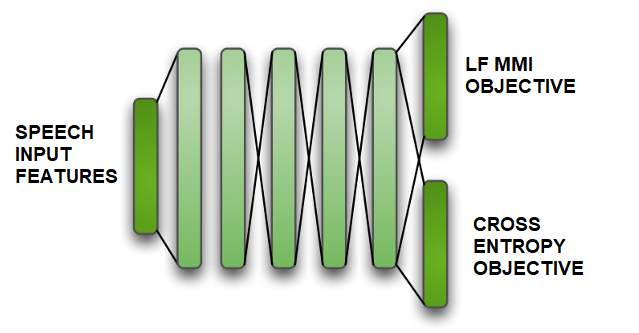
\includegraphics[width=0.7\textwidth]{img/LFMMI-crossent.png}
    \caption{LFMMI input objectives}
    \label{fig:LFMMI-INPUT}
\end{figure}



\begin{table}[h!]
    \centering
    \caption{Our Results} 
    \label{tab:our_result}

    \begin{tabularx}{\textwidth} { 
  | >{\raggedright\arraybackslash}X 
  | >{\raggedright\arraybackslash}X 
  | >{\raggedright\arraybackslash}X | }
    \hline
    \textbf{Data-set} & \textbf{METHOD} & \textbf{RESULTS} \\
    \hline
    250 words each by 10 speakers\newline 100+86 words by 5 speakers\newline PRUS \cite{qureshi_urdu_2021} 708 sentences with 7 speakers\newline & HMM GMM TRIPHONE & WER 13\% and SER 31.2\%  \\ 
    \hline
    250 words each by 10 speakers\newline 100+86 words by 5 speakers\newline PRUS 708 sentences with 7 speakers \cite{zia_pronouncur_2018}\newline & TRIPHONE WITH CNN-TDNN & WER 5.2\% and SER 20.45\%  \\
    \hline
    CPLC (unseen random call) data-set & TRIPHONE WITH CNN-TDNN & 5.2\% on parts with no overlaps and better volumes. In overlapping speech and OOV scenario, WER was 58\% \\   
    \hline
    \end{tabularx}    
\end{table}



\section{ASR for noisy environment}
Speech recognizers may require the speech to be clean from environmental noises, acoustic distortions, microphones, and transmission channel distortions or they may ideally handle any of these problems. While current speech recognizer gives an acceptable performance in carefully controlled environments, their performance degrades rapidly when they are applied in noisy environments. 

This noise can take the form of speech from other speakers; equipment sounds, air conditioners, background voices, bad mic or others. The noise might also be created by the speaker himself in a form of lip smacks, coughs or sneezes. Separating speech from background noise is one essential problem for the ASR system when working in a telephonic call center environment.

Another constant problem is Speech overlapping i.e. that several people are talking at the same time. Researchers observed a vital degradation in the performance of ASR systems when speech contained cross-talk. Some of the approaches taken to this are: \cite{alharbi_automatic_2021}

\begin{itemize}
    \item A target speaker extraction network (TEnet) that identifies and isolates a specific speaker's speech based on a clean voice sample of the speaker to address the problem of multiple people speaking at the same time. This method has a high performance with a word error rate (WER) of 22.5\% and signal-to-distortion rate (SDR) of 15.5\%. 
    \item Another model is to divide the interfering speech recognition problem in one channel into three parts: translation, speaker tracking, and speech recognition. This is said to improve the performance by 30\% the rate of speech errors. 
    \item Another model combined the above approaches to address the cross-talk problem called deep clustering (DPCL) by creating a hybrid acoustic model. This gave a WER of 16.5\% on the Wall Street Journal "wsj0-2mix" dataset.    
\end{itemize}

\subsection{Noisy Channel Model}
\label{sub:noisy_channel_model}

In information theory, Shannon's Noisy-Channel Coding Theorem states that it is possible to communicate over a noisy channel with arbitrarily small chance of error when the rate of communication is kept below a maximum which is constant for a channel.

The noisy channel model is a framework used in spell checkers, question answering, speech recognition, and machine translation. In this model, the goal is to find the intended word given a word where the letters have been scrambled in some manner.

The noisy channel model involves searching through space of all possible sentences in the dictionary, picking the one that is most probable given the waveform, using the acoustic model to give a set of likely phone Sequences and using the lexical and language models to judge which of these are likely to result in probable word sequences. This is done with sophisticated algorithms to juggle the statistics and looks more like the rule-based approach except that it is all learned automatically from data. \cite{jurafsky_speech_2009} Our idea was to introduce a mix of clean and noisy (low quality) data to see if the system is able to predict words accurately from telephonic-type of audio.
\par
\vspace{11pt}
So, if we have an alphabet $\Sigma$. \newline
\vspace{11pt}
If $\Sigma^*$ is set of finite strings over $\Sigma$. \newline
\vspace{11pt}
S is dictionary of valid words which is subset of $\Sigma^*$ i.e $D \subseteq \Sigma^*$ \newline
\vspace{11pt}
The noisy channel is the matrix: \newline 
\begin{equation*}
    \Gamma_{ws} = Pr(s|w)
\end{equation*} 
\vspace{11pt}
where $w \in D$ is the intended words and $S \in \Sigma^*$ is the scrambled actually received.  \cite{brill_improved_2000} 
\vspace{11pt}
For instance If $\Sigma$ contains all English alphabets and English Dictionary is $D \subseteq \Sigma^*$. There can be several losses in the telephonic line like: 
\begin{itemize}
    \item Missing phones - E.g Hello understood or relayed as Hell due to missing /o/ 
    \item Accidental additions of letters e.g. The word "miss" received as Missing
    \item Swapping letters e.g. their vs thier (if looking for character level accuracy)
    \item Replacing Letter e.g. N in snack replaced with  M making the word smack
\end{itemize}

To construct the noisy channel $\Gamma$ we must consider probability of each mistake given in intended word ($Pr(s|w)$ for all $w \in D$ and $s \in \Sigma^*$). 

%These probabilities may be gathered, for example, by considering the Damerau–Levenshtein distance between s and w or by comparing the draft of an essay with one that has been manually edited for spelling.

The goal of the noisy channel model is to find the intended word given the scrambled word that was received. The decision function $\sigma:\Sigma^* \rightarrow D$ is a function that, given a scrambled word, returns the intended word.

Methods of constructing a decision function include the maximum likelihood rule, the maximum a posteriori rule, and the minimum distance rule. In some cases, it may be better to accept the scrambled word as the intended word rather than attempt to find an intended word in the dictionary. For example, the word "Fantabulicious" may not be in the dictionary, but might in fact be the intended word.  

All Morphology based approaches aim to reduce ASR errors by reducing the OOV rate through modeling at the morph level and also cover for lack of available wide-vocabulary data since we cannot always arrange for an audio dataset for every possible word in the dictionary. Morph-based language modelling uses morphs instead of words but it may require longer context (since multiple morphs correspond to one word) \cite{creutz_morph-based_2007}